% IDS Paper — arXiv preprint (NeurIPS 2026 base style, [preprint] option)
\documentclass{article}

% arXiv preprint: de-anonymized, no "Under review" banner, no line numbers.
% Swap to default (no option) for double-blind submission, or [main, final] for camera-ready.
\usepackage[preprint]{neurips_2026}
% \usepackage{neurips_2026}
% \usepackage[main, final]{neurips_2026}

\usepackage[utf8]{inputenc}
\usepackage[T1]{fontenc}
\usepackage[colorlinks=true,
            allcolors=blue!55!black]{hyperref}
\renewcommand{\sectionautorefname}{\S}
\renewcommand{\subsectionautorefname}{\S}
\renewcommand{\subsubsectionautorefname}{\S}

\usepackage{url}
\usepackage{booktabs}
\usepackage{amsfonts}
\usepackage{nicefrac}
\usepackage{microtype}
\usepackage[table]{xcolor}
\usepackage{xspace}
\usepackage{enumitem}
\usepackage{amsmath,amssymb}
\usepackage{multirow}
\usepackage{pifont}
\providecommand{\cmark}{\ding{51}}
\providecommand{\xmark}{\ding{55}}
\usepackage{cleveref}
\usepackage{algorithm}
\usepackage{algpseudocode}
\usepackage{graphicx}
\usepackage{subcaption}
\usepackage{tabularx}
\usepackage{tikz}
\usepackage{wrapfig}
\usetikzlibrary{arrows.meta,calc,positioning}
\usepackage{listings}

% Coq listing setup
\lstdefinelanguage{Coq}{
  morekeywords={Module, Type, End, Definition, Fixpoint, Parameter, Axiom,
                Theorem, Lemma, Proof, Qed, Admitted, forall, fun, match,
                with, if, then, else, let, in, return, true, false, nil,
                Some, None, intros, unfold, simpl, reflexivity, induction,
                apply, rewrite, destruct, split, constructor, inversion,
                assumption, tauto, Require, Import, Inductive, Fixpoint},
  sensitive=true,
  morecomment=[s]{(*}{*)},
  morestring=[b]",
}
\lstset{
  language=Coq,
  basicstyle=\ttfamily\footnotesize,
  keywordstyle=\bfseries,
  commentstyle=\itshape\color{gray!50!black},
  showstringspaces=false,
  columns=fullflexible,
  breaklines=true,
  frame=single,
  framesep=4pt,
  xleftmargin=4pt,
  xrightmargin=4pt,
  aboveskip=4pt,
  belowskip=4pt,
}

% \providecommand{\aknew}[1]{{\color{red}{#1}}}
\providecommand{\aknew}[1]{#1}

% Comment system
\definecolor{cldarkgreen}{rgb}{0.0, 0.6, 0.2}  % darker than default green
\newif\ifcomments
\commentsfalse
\ifcomments
    \providecommand{\shubham}[1]{{\color{blue}{/* shubham: #1 */}}}
    \providecommand{\mert}[1]{{\color{olive}{/* mert: #1 */}}}
    \providecommand{\shu}[1]{{\color{magenta}{/* shu: #1 */}}}
    \providecommand{\ion}[1]{{\color{cyan}{/* ion: #1 */}}}
    \providecommand{\ak}[1]{{\color{orange}{/* alex: #1 */}}}
    \providecommand{\mz}[1]{{\color{purple}{/* mz: #1 */}}}
    \providecommand{\mohsen}[1]{{\color{orange}{/* mohsen: #1 */}}}
    \providecommand{\accheng}[1]{{\color{red}{/* accheng: #1 */}}}
    \providecommand{\cl}[1]{{\textcolor{cldarkgreen}{/* cl: #1 */}}}
    % \providecommand{\aknew}[1]{{\color{red}{#1}}}
\else
    \providecommand{\shubham}[1]{}
    \providecommand{\mert}[1]{}
    \providecommand{\shu}[1]{} 
    \providecommand{\ion}[1]{}
    \providecommand{\ak}[1]{}
    \providecommand{\mohsen}[1]{}
    \providecommand{\accheng}[1]{}
    \providecommand{\cl}[1]{}
    % \providecommand{\aknew}[1]{#1}
\fi

% Custom macros
% \newcommand{\sys}{VibeProof\xspace}
% \newcommand{\sys}{CertGen\xspace}
% \newcommand{\sys}{CerSyn\xspace}
% \newcommand{\sys}{AC\'{E}S\xspace}
\newcommand{\sys}{IDS\xspace}
\newcommand{\sysname}{\sys}
\usepackage{tipa}
\newcommand{\syspronounce}{\textipa{["eIs\textepsilon z]}\xspace}
\newcommand{\coq}{Rocq\xspace}
\newcommand{\TODO}[1]{{\color{red}\textbf{TODO:} #1}}
\newcommand{\eg}{\emph{e.g.,}\xspace}
\newcommand{\ie}{\emph{i.e.,}\xspace}
\newcommand{\etal}{\emph{et~al.}\xspace}


\usepackage{xcolor}
\definecolor{softred}{HTML}{CC0000}
\definecolor{softgreen}{HTML}{2AAA2A}
\definecolor{softyellow}{HTML}{B8860B}
\newcommand{\red}[1]{\textcolor{softred}{#1}}
\newcommand{\green}[1]{\textcolor{softgreen}{#1}}
\newcommand{\yellow}[1]{\textcolor{softyellow}{#1}}

% Figure-reference numbered badge -- inline blue circle matching Fig 3 numbering
\definecolor{fignumcolor}{HTML}{3B78D9}
\DeclareRobustCommand{\fignum}[1]{\tikz[baseline=(c.base)]{\node[circle, fill=fignumcolor, text=white, inner sep=0.4pt, minimum size=8pt, font=\sffamily\bfseries\tiny] (c) {#1};}}

% Standardize section references to use \S
\crefformat{section}{\S#2#1#3}
\crefformat{subsection}{\S#2#1#3}
\crefformat{subsubsection}{\S#2#1#3}
\Crefformat{section}{\S#2#1#3}
\Crefformat{subsection}{\S#2#1#3}
\Crefformat{subsubsection}{\S#2#1#3}
\crefrangeformat{section}{\S#3#1#4--\S#5#2#6}
\crefrangeformat{subsection}{\S#3#1#4--\S#5#2#6}
\crefmultiformat{section}{\S\S#2#1#3}{ and~#2#1#3}{, #2#1#3}{ and~#2#1#3}
\crefmultiformat{subsection}{\S\S#2#1#3}{ and~#2#1#3}{, #2#1#3}{ and~#2#1#3}

% Appendix reference formats (must be declared in preamble so body
% references like \cref{app:foo} render correctly; the matching
% \crefalias is set after \appendix below so labels typed as appendix.)
\crefformat{appendix}{App.~#2#1#3}
\Crefformat{appendix}{App.~#2#1#3}
\crefrangeformat{appendix}{App.~#3#1#4--#5#2#6}
\crefmultiformat{appendix}{App.~#2#1#3}{ and~#2#1#3}{, #2#1#3}{ and~#2#1#3}
\crefformat{subappendix}{App.~#2#1#3}
\Crefformat{subappendix}{App.~#2#1#3}
\crefformat{subsubappendix}{App.~#2#1#3}
\Crefformat{subsubappendix}{App.~#2#1#3}

% Figure/table reference formats: capitalize for professional appearance
% (cleveref's default is lowercase "fig."/"table" -- override to "Fig."/"Table")
\crefformat{figure}{Fig.~#2#1#3}
\Crefformat{figure}{Fig.~#2#1#3}
\crefrangeformat{figure}{Figs.~#3#1#4--#5#2#6}
\crefmultiformat{figure}{Figs.~#2#1#3}{ and~#2#1#3}{, #2#1#3}{ and~#2#1#3}
\crefformat{table}{Table~#2#1#3}
\Crefformat{table}{Table~#2#1#3}
\crefrangeformat{table}{Tables~#3#1#4--#5#2#6}
\crefmultiformat{table}{Tables~#2#1#3}{ and~#2#1#3}{, #2#1#3}{ and~#2#1#3}


\newcommand{\cut}[1]{\unskip}
% \newcommand{\cut}[1]{#1}



% -------------------------------------
% imports for specs

\usepackage{mathpartir}

\usepackage{graphicx}

% \usepackage[firstpage]{draftwatermark}
% % \SetWatermarkText{\hspace*{8in}\raisebox{3.5in}{\includegraphics[scale=0.1]{aec-badge-popl.pdf}}}
% \SetWatermarkText{\hspace*{13.3in}\raisebox{-6.5in}{\includegraphics[scale=0.1]{aec-badge-popl.pdf}}}
% \SetWatermarkAngle{0}

%--------------------------------------
% To use \mathbb
\usepackage{amsfonts}
%--------------------------------------
% To defined theorems and Lemmas
 \usepackage{amsthm} 
\theoremstyle{definition}  % non-italic
% Definition, Lemma and Theorem
\newtheorem{definition}{Definition}
\newtheorem{theorem}{Theorem}
% \newtheorem{definition}{Lemma}
\newtheorem{lemma}{Lemma}
\newtheorem{corollary}{Corollary}
%--------------------------------------
% To have colored annotations
\usepackage{xcolor}
%--------------------------------------
% To strike out text
\usepackage[normalem]{ulem}
\usepackage{cancel}
%--------------------------------------
%\usepackage{hyperref}
\usepackage{url}
%--------------------------------------
% Programming language rules
\usepackage{mmm}
\usepackage{pl}
%--------------------------------------
% Arrow symbols 
\let\Bbbk\relax
\usepackage{amssymb}
%--------------------------------------
% \xrightarrow
\usepackage{amsmath}
%--------------------------------------
% % To write algorithms
% \usepackage{algorithm}
% %\usepackage{algpseudocode}
% \usepackage[noend]{algpseudocode}
% \let\algState\State
% \usepackage{varwidth}% http://ctan.org/pkg/varwidth
% % To have Algorithm float
% % \usepackage{algorithm}
% % To make the algorithms float to the top
% \usepackage{float}
% \newfloat{algorithm}{t}{lop}
% %\renewcommand{\algorithmicforall}{\textbf{foreach}}
%--------------------------------------

% this employs smarter hyphenations, par, and other rules
% ... and helps condense the paper
\usepackage{microtype}

% To remove a warning for fonts
% \usepackage{lmodern}% http://ctan.org/pkg/lm

%--------------------------------------
% Symbol definitions and comments
% Standard
\def\t{\phantom{X}}

\def\<{\langle}
\def\>{\rangle}

%--------------------------------------

\usepackage{listings}
\lstset{
   language=C,
   captionpos=b,
   tabsize=3,
%   frame=lines,
%   keywordstyle=\color{blue},
%   commentstyle=\color{darkgreen},
%   stringstyle=\color{red},
   numbers=left,
   numberstyle=\tiny,
   numbersep=5pt,
   breaklines=true,
   showstringspaces=false,
%   basicstyle=\small\bfseries,
   basicstyle=\small\ttfamily,
   emph={label}
}

\usepackage{array}

\usepackage{tikz}
\usetikzlibrary{positioning} 
\usetikzlibrary{arrows} 
%\usetikzlibrary{graphs} % Not supported by tikz 2.10
\usetikzlibrary{calc}
\usetikzlibrary{backgrounds}
\usetikzlibrary{shapes}

%\usepackage{caption}
%\usepackage{subcaption}

\usepackage{stmaryrd}

\def\defeq{\triangleq}

\def\self{\mathit{self}}

\def\switch{\mathsf{switch} \ }
\def\case{\mathsf{case} \ }
\def\ret{\mathsf{ret} \ }
\def\lforall{\mathsf{forall} \ }
\def\lif{\mathsf{if} \ }
\def\lelse{\mathsf{else} \ }
\def\lmap{\mathsf{map} \ }
\def\llet{\mathsf{let} \ }
\def\max{\mathsf{max}}

\def\vc{\mathit{vc}}
\def\List{\mathsf{List}}
\def\llookup{\mathsf{lookup} \ }

\def\RYW{\mathit{RYW}}
\def\MR{\mathit{MR}}
\def\WFR{\mathit{WFR}}
\def\MW{\mathit{MW}}
\def\CC{\mathit{CC}}
\def\LCC{\mathit{LCC}}
\def\Rel{\mathit{Rel}}

\def\ext{\mathsf{ext}}

\def\CState{\mathsf{CState}}
\def\RState{\mathsf{RState}}

\def\true{\mathsf{true}}
\def\Set{\mathsf{Set}}
\def\Nat{\mathsf{Nat}}
% \def\L{\mathsf{L}}
\def\L{L}
\def\lab{\mathit{label}}
\def\clientLabs{\mathit{client\text{-}labels}}

\def\cInit{\mathsf{c\text{-}init}}
\def\rInit{\mathsf{r\text{-}init}}

\def\get{\mathsf{get}}
\def\getGuard{\mathsf{get\text{-}guard}}
\def\getReq{\mathsf{get\text{-}req}}
\def\getRes{\mathsf{get\text{-}res}}

\def\lput{\mathsf{put}}
\def\putGuard{\mathsf{put\text{-}guard}}
\def\putReq{\mathsf{put\text{-}req}}
\def\putRes{\mathsf{put\text{-}res}}

\def\Type{\mathsf{Type}}
\def\Option{\mathsf{Option}}
\def\Bool{\mathsf{Bool}}

\def\Event{\mathit{Event}}
\def\Req{\mathit{Req}}
\def\req{\mathit{req}}

\def\Res{\mathit{Res}}
\def\res{\mathit{res}}

\def\PutReq{\mathit{Put\text{-}req}}
\def\PutReqPayload{\mathsf{Put\text{-}req\text{-}payload}}
\def\PutRes{\mathit{Put\text{-}res}}
\def\PutResPayload{\mathsf{Put\text{-}res\text{-}payload}}

\def\GetReq{\mathit{Get\text{-}req}}
\def\GetReqPayload{\mathsf{Get\text{-}req\text{-}payload}}
\def\GetRes{\mathit{Get\text{-}res}}
\def\GetResPayload{\mathsf{Get\text{-}res\text{-}payload}}

\def\Unit{\mathsf{Unit}}

% Program Syntax

% Uses:
% $
% \sPut{}{},
% \sPut{k}{v},
% \sPut[i]{k}{v},
% % 
% \sGet{}{},
% \sGet{x}{k},
% \sGet[i]{x}{k},
% $

\newcommand\sPut[3][]{%
  \mathit{put}%
  \ifthenelse{\equal{#1}{}}{%
    \ifthenelse{\equal{#2}{}}{}{
    ({#2},{#3})}%
  }{%
    ^{#1}({#2},{#3})%
  }%
}  
  
\newcommand\sGet[3][]{%
   \ifthenelse{\equal{#2}{}}{}{#2\leftarrow}%
   \mathit{get}
   \ifthenelse{\equal{#1}{}}{}{^{#1}}%
   \ifthenelse{\equal{#3}{}}{}{({#3})}}

% \newcommand\sGet[2][]{%
%     \ifthenelse{\equal{#1}{}}{}{#1\leftarrow }%
%     \mathit{get}%
%     \ifthenelse{\equal{#2}{}}{}{({#2})}}
    
  \newcommand\sSkip{\mathit{skip}}

\newcommand{\name}[1]{\textsc{#1}}

\newcommand\indrule[3][]{%
%  \inferrule*[Right=#1]{#2}{#3}%
  \inferrule[#1]{#2}{#3}%
  }

\newcommand\figurealgtextsize{%
%   \small%
  \setlength{\abovedisplayskip}{0pt}%
  \setlength{\abovedisplayshortskip}{0pt}%
  \setlength{\belowdisplayskip}{0pt}%
  \setlength{\belowdisplayshortskip}{0pt}}
\newcommand\figureruletextsize{%
%   \small
  \setlength{\abovedisplayskip}{0pt}%
  \setlength{\abovedisplayshortskip}{0pt}%
  \setlength{\belowdisplayskip}{0pt}%
  \setlength{\belowdisplayshortskip}{0pt}
}
\newcommand\figuredefstextsize{%
%   \small
%  \large  
  \setlength{\abovedisplayskip}{0pt}%
  \setlength{\abovedisplayshortskip}{0pt}%
  \setlength{\belowdisplayskip}{0pt}%
  \setlength{\belowdisplayshortskip}{0pt}
}

\usepackage{siunitx}  % To format numbers

\setlength{\textfloatsep}{20pt}

\usepackage{balance}

% \newfont{\mycrnotice}{ptmr8t at 7pt}
% \newfont{\myconfname}{ptmri8t at 7pt}
% \let\crnotice\mycrnotice%
% \let\confname\myconfname%

\newcommand\world[3]{%
   {\begin{array}{l} ( %\left(
      #1, \\ \phantom{(}
      #2, \\ \phantom{(}
      #3          
   ) \end{array}}
}  

\newcommand\note[1]{\text{\small#1}}
\newcommand\bnote[1]{\textbf{\small#1}}

% \newcommand\note[1]{\footnotesize\text{#1}}
% \newcommand\bnote[1]{\footnotesize\textbf{#1}}

\usepackage{tikz}
\usetikzlibrary{positioning, arrows.meta}

%%%%%%%%%%%%%%%%%%%%%%%%%%%%%%%%%%%%%%%%%%%%%%%%%%%%%%%%%%%%%%%%%%%%%%%%%%%%%%
% Unicode symbols to be used with pdflatex and Sphinx
%%%%%%%%%%%%%%%%%%%%%%%%%%%%%%%%%%%%%%%%%%%%%%%%%%%%%%%%%%%%%%%%%%%%%%%%%%%%%%

% In Emacs `C-u C-x =` gives the symbol information. We use of
% hexadecimal code point.

% Requires `\usepackage[utf8]{inputenc}` with some versions of
% `pdflatex`.

% We use the `textcomp` package because the `sphinx.sty` also uses it.

% You can find the LaTeX command for a Unicode code point in
% http://unicode.scarfboy.com/ or
% https://www.johndcook.com/unicode_latex.html .

% Making upper and lower case script characters in math mode. From
% http://www.peteryu.ca/tutorials/publishing/latex_math_script_styles
% and
% https://tex.stackexchange.com/questions/58098/what-are-all-the-font-styles-i-can-use-in-math-mode.
\DeclareMathAlphabet{\mathpzc}{OT1}{pzc}{m}{it}

%%%%%%%%%%%%%%%%%%%%%%%%%%%%%%%%%%%%%%%%%%%%%%%%%%%%%%%%%%%%%%%%%%%%%%%%%%%%%%
% Please keep the below list ordered by code points!

\DeclareUnicodeCharacter{00AC}{\ensuremath{\neg}}                     % Symbol ¬
\DeclareUnicodeCharacter{00B1}{\ensuremath{\pm}}                      % Symbol ±
\DeclareUnicodeCharacter{00B2}{\ensuremath{^2}}                       % Symbol ²
\DeclareUnicodeCharacter{00B3}{\ensuremath{^3}}                       % Symbol ³
\DeclareUnicodeCharacter{00B7}{\ensuremath{\cdot}}                    % Symbol ·
\DeclareUnicodeCharacter{00B9}{\ensuremath{^1}}                       % Symbol ¹
\DeclareUnicodeCharacter{00D7}{\ensuremath{\times}}                   % Symbol ×
\DeclareUnicodeCharacter{02B0}{\ensuremath{^h}}                       % Symbol ʰ
\DeclareUnicodeCharacter{02B3}{\ensuremath{^r}}                       % Symbol ʳ
\DeclareUnicodeCharacter{02E2}{\ensuremath{^s}}                       % Symbol ˢ
\DeclareUnicodeCharacter{20F0}{\ensuremath{^*}}                       % Symbol  ⃰ 
\DeclareUnicodeCharacter{0302}{\ensuremath{\hat{\phantom{x}}}}        % Symbol ̂
\DeclareUnicodeCharacter{0332}{\ensuremath{\underline{\phantom{x}}}}  % Symbol ̲
\DeclareUnicodeCharacter{0308}{\ensuremath{\ddot{\phantom{x}}}}       % Symbol ̈
\DeclareUnicodeCharacter{0393}{\ensuremath{\Gamma}}                   % Symbol Γ
\DeclareUnicodeCharacter{0394}{\ensuremath{\Delta}}                   % Symbol Δ
\DeclareUnicodeCharacter{0398}{\ensuremath{\Theta}}                   % Symbol Θ
\DeclareUnicodeCharacter{039B}{\ensuremath{\Lambda}}                  % Symbol Λ
\DeclareUnicodeCharacter{039E}{\ensuremath{\Xi}}                      % Symbol Ξ
\DeclareUnicodeCharacter{03A0}{\ensuremath{\Pi}}                      % Symbol Π
\DeclareUnicodeCharacter{03A3}{\ensuremath{\Sigma}}                   % Symbol Σ

% There is not `\Tau` command in LaTeX, so we use `\mathrm{T}`. See
% http://tex.stackexchange.com/questions/1368/why-can-i-only-use-some-capital-greek-letters-inside-my-equations.
\DeclareUnicodeCharacter{03A4}{\ensuremath{\mathrm{T}}}  % Symbol Τ

\DeclareUnicodeCharacter{03A5}{\ensuremath{\Upsilon}}   % Symbol Υ
\DeclareUnicodeCharacter{03A6}{\ensuremath{\Phi}}       % Symbol Φ
\DeclareUnicodeCharacter{03A8}{\ensuremath{\Psi}}       % Symbol Ψ
\DeclareUnicodeCharacter{03A9}{\ensuremath{\Omega}}     % Symbol Ω
\DeclareUnicodeCharacter{03B1}{\ensuremath{\alpha}}     % Symbol α
\DeclareUnicodeCharacter{03B2}{\ensuremath{\beta}}      % Symbol β
\DeclareUnicodeCharacter{03B3}{\ensuremath{\gamma}}     % Symbol γ
\DeclareUnicodeCharacter{03B4}{\ensuremath{\delta}}     % Symbol δ
\DeclareUnicodeCharacter{03B5}{\ensuremath{\epsilon}}   % Symbol ε
\DeclareUnicodeCharacter{03B6}{\ensuremath{\zeta}}      % Symbol ζ
\DeclareUnicodeCharacter{03B7}{\ensuremath{\eta}}       % Symbol η
\DeclareUnicodeCharacter{03B8}{\ensuremath{\theta}}     % Symbol θ
\DeclareUnicodeCharacter{03B9}{\ensuremath{\iota}}      % Symbol ι
\DeclareUnicodeCharacter{03BA}{\ensuremath{\kappa}}     % Symbol κ
\DeclareUnicodeCharacter{03BB}{\ensuremath{\lambda}}    % Symbol λ
\DeclareUnicodeCharacter{03BC}{\ensuremath{\mu}}        % Symbol μ
\DeclareUnicodeCharacter{03BD}{\ensuremath{\nu}}        % Symbol ν
\DeclareUnicodeCharacter{03BE}{\ensuremath{\xi}}        % Symbol ξ
\DeclareUnicodeCharacter{03C0}{\ensuremath{\pi}}        % Symbol π
\DeclareUnicodeCharacter{03C1}{\ensuremath{\rho}}       % Symbol ρ
\DeclareUnicodeCharacter{03C2}{\ensuremath{\varsigma}}  % Symbol ς
\DeclareUnicodeCharacter{03C3}{\ensuremath{\sigma}}     % Symbol σ
\DeclareUnicodeCharacter{03C4}{\ensuremath{\tau}}       % Symbol τ
\DeclareUnicodeCharacter{03C5}{\ensuremath{\upsilon}}   % Symbol υ
\DeclareUnicodeCharacter{03C6}{\ensuremath{\varphi}}    % Symbol φ
\DeclareUnicodeCharacter{03C7}{\ensuremath{\chi}}       % Symbol χ
\DeclareUnicodeCharacter{03C8}{\ensuremath{\psi}}       % Symbol ψ
\DeclareUnicodeCharacter{03C9}{\ensuremath{\omega}}     % Symbol ω
\DeclareUnicodeCharacter{03D1}{\ensuremath{\vartheta}}  % Symbol ϑ

\DeclareUnicodeCharacter{0432}{\ensuremath{\mathrm{PDF\;TODO}}}  % Symbol в
\DeclareUnicodeCharacter{0435}{\ensuremath{\mathrm{PDF\;TODO}}}  % Symbol е
\DeclareUnicodeCharacter{0438}{\ensuremath{\mathrm{PDF\;TODO}}}  % Symbol и
\DeclareUnicodeCharacter{043C}{\ensuremath{\mathrm{PDF\;TODO}}}  % Symbol м
\DeclareUnicodeCharacter{0440}{\ensuremath{\mathrm{PDF\;TODO}}}  % Symbol р
\DeclareUnicodeCharacter{0442}{\ensuremath{\mathrm{PDF\;TODO}}}  % Symbol т
\DeclareUnicodeCharacter{041F}{\ensuremath{\mathrm{PDF\;TODO}}}  % Symbol П
\DeclareUnicodeCharacter{0BA8}{\ensuremath{\mathrm{PDF\;TODO}}}  % Symbol ந
\DeclareUnicodeCharacter{0BBF}{\ensuremath{\mathrm{PDF\;TODO}}}  % Symbol  ி
\DeclareUnicodeCharacter{1100}{\ensuremath{\mathrm{PDF\;TODO}}}  % Symbol ᄀ
\DeclareUnicodeCharacter{11F9}{\ensuremath{\mathrm{PDF\;TODO}}}  % Symbol ᇹ

\DeclareUnicodeCharacter{1D48}{\ensuremath{^d}}  % Symbol ᵈ
\DeclareUnicodeCharacter{1D50}{\ensuremath{^m}}  % Symbol ᵐ
\DeclareUnicodeCharacter{1D56}{\ensuremath{^p}}  % Symbol ᵖ
\DeclareUnicodeCharacter{1D62}{\ensuremath{_i}}  % Symbol ᵢ
\DeclareUnicodeCharacter{1D63}{\ensuremath{_r}}  % Symbol ᵣ
\DeclareUnicodeCharacter{1D64}{\ensuremath{_u}}  % Symbol ᵤ
\DeclareUnicodeCharacter{1D9C}{\ensuremath{^c}}  % Symbol ᶜ


% The command `\text` requires `\usepackage{amsmath}` and the command
% `\textasciiacute` requires `\usepackage{textcomp}`.

\DeclareUnicodeCharacter{2032}{\ensuremath{\text{\textasciiacute}}}  % Symbol ′

\DeclareUnicodeCharacter{2070}{\ensuremath{^0}}  % Symbol ⁰
\DeclareUnicodeCharacter{2074}{\ensuremath{^4}}  % Symbol ⁴
\DeclareUnicodeCharacter{2075}{\ensuremath{^5}}  % Symbol ⁵
\DeclareUnicodeCharacter{2076}{\ensuremath{^6}}  % Symbol ⁶
\DeclareUnicodeCharacter{2077}{\ensuremath{^7}}  % Symbol ⁷
\DeclareUnicodeCharacter{2078}{\ensuremath{^8}}  % Symbol ⁸
\DeclareUnicodeCharacter{2079}{\ensuremath{^9}}  % Symbol ⁹
\DeclareUnicodeCharacter{207A}{\ensuremath{^+}}  % Symbol ⁺
\DeclareUnicodeCharacter{207B}{\ensuremath{^-}}  % Symbol ⁻
\DeclareUnicodeCharacter{207F}{\ensuremath{^n}}  % Symbol ⁿ
\DeclareUnicodeCharacter{2080}{\ensuremath{_0}}  % Symbol ₀
\DeclareUnicodeCharacter{2081}{\ensuremath{_1}}  % Symbol ₁
\DeclareUnicodeCharacter{2082}{\ensuremath{_2}}  % Symbol ₂
\DeclareUnicodeCharacter{2083}{\ensuremath{_3}}  % Symbol ₃
\DeclareUnicodeCharacter{2084}{\ensuremath{_4}}  % Symbol ₄
\DeclareUnicodeCharacter{2085}{\ensuremath{_5}}  % Symbol ₅
\DeclareUnicodeCharacter{2086}{\ensuremath{_6}}  % Symbol ₆
\DeclareUnicodeCharacter{2087}{\ensuremath{_7}}  % Symbol ₇
\DeclareUnicodeCharacter{2088}{\ensuremath{_8}}  % Symbol ₈
\DeclareUnicodeCharacter{2089}{\ensuremath{_9}}  % Symbol ₉
\DeclareUnicodeCharacter{208A}{\ensuremath{_+}}  % Symbol ₊
\DeclareUnicodeCharacter{208B}{\ensuremath{_-}}  % Symbol ₋
\DeclareUnicodeCharacter{2090}{\ensuremath{_a}}  % Symbol ₐ
\DeclareUnicodeCharacter{2091}{\ensuremath{_e}}  % Symbol ₑ
\DeclareUnicodeCharacter{2095}{\ensuremath{_h}}  % Symbol ₕ
\DeclareUnicodeCharacter{2096}{\ensuremath{_k}}  % Symbol ₖ
\DeclareUnicodeCharacter{2097}{\ensuremath{_l}}  % Symbol ₗ
\DeclareUnicodeCharacter{2098}{\ensuremath{_m}}  % Symbol ₘ
\DeclareUnicodeCharacter{2099}{\ensuremath{_n}}  % Symbol ₙ
\DeclareUnicodeCharacter{209A}{\ensuremath{_p}}  % Symbol ₚ
\DeclareUnicodeCharacter{2092}{\ensuremath{_o}}  % Symbol ₒ
\DeclareUnicodeCharacter{209B}{\ensuremath{_s}}  % Symbol ₛ
\DeclareUnicodeCharacter{209C}{\ensuremath{_t}}  % Symbol ₜ
\DeclareUnicodeCharacter{2093}{\ensuremath{_x}}  % Symbol ₓ

% \DeclareUnicodeCharacter{2113}{\ensuremath{\mathpzc{l}}} % Symbol ℓ
\DeclareUnicodeCharacter{2113}{\ensuremath{\ell}} % Symbol ℓ

% The command `\mathbbm` requires `\usepackage{bbm}`.
\DeclareUnicodeCharacter{2115}{\ensuremath{\mathbbm{N}}}  % Symbol ℕ
\DeclareUnicodeCharacter{211A}{\ensuremath{\mathbbm{Q}}}  % Symbol ℚ
\DeclareUnicodeCharacter{211D}{\ensuremath{\mathbbm{R}}}  % Symbol ℝ
\DeclareUnicodeCharacter{2124}{\ensuremath{\mathbbm{Z}}}  % Symbol ℤ

\DeclareUnicodeCharacter{2135}{\ensuremath{\aleph}}           % Symbol ℵ
\DeclareUnicodeCharacter{2190}{\ensuremath{\leftarrow}}       % Symbol ←
\DeclareUnicodeCharacter{2192}{\ensuremath{\rightarrow}}      % Symbol →
\DeclareUnicodeCharacter{2194}{\ensuremath{\leftrightarrow}}  % Symbol ↔

% The command `\twoheadrightarrow` requires `\usepackage{amssymb}`.
\DeclareUnicodeCharacter{21A0}{\ensuremath{\twoheadrightarrow}}  % Symbol ↠

\DeclareUnicodeCharacter{21A6}{\ensuremath{\mapsto}}  % Symbol ↦
\DeclareUnicodeCharacter{21A6}{\ensuremath{\mapsto}}  % Symbol ↦

% The command `\restriction` requires `\usepackage{amssymb}`.
\DeclareUnicodeCharacter{21BE}{\ensuremath{\restriction}}  % Symbol ↾

\DeclareUnicodeCharacter{21D0}{\ensuremath{\Leftarrow}}       % Symbol ⇐
\DeclareUnicodeCharacter{21D2}{\ensuremath{\Rightarrow}}      % Symbol ⇒
\DeclareUnicodeCharacter{21D4}{\ensuremath{\Leftrightarrow}}  % Symbol ⇔

\DeclareUnicodeCharacter{2200}{\ensuremath{\forall}}      % Symbol ∀
\DeclareUnicodeCharacter{2203}{\ensuremath{\exists}}      % Symbol ∃
\DeclareUnicodeCharacter{2204}{\ensuremath{\not\exists}}  % Symbol ∃
\DeclareUnicodeCharacter{2205}{\ensuremath{\emptyset}}    % Symbol ∅
\DeclareUnicodeCharacter{2208}{\ensuremath{\in}}          % Symbol ∈
\DeclareUnicodeCharacter{2209}{\ensuremath{\not\in}}      % Symbol ∉
\DeclareUnicodeCharacter{220B}{\ensuremath{\ni}}          % Symbol ∋
\DeclareUnicodeCharacter{220C}{\ensuremath{\not\ni}}      % Symbol ∌

% The command `\blacksquare` requires `\usepackage{amssymb}`.
\DeclareUnicodeCharacter{220E}{{\tiny \ensuremath{\blacksquare}}} % Symbol ∎

\DeclareUnicodeCharacter{220F}{{\tiny \ensuremath{\prod}}}  % Symbol ∏
\DeclareUnicodeCharacter{2211}{\ensuremath{\sum}}           % Symbol ∑
% 2218
\DeclareUnicodeCharacter{25CB}{\ensuremath{\circ}}          % Symbol ∘
% \DeclareUnicodeCharacter{2219}{\ensuremath{\bullet}}        % Symbol ∙
\DeclareUnicodeCharacter{2022}{\ensuremath{\bullet}}        % Symbol •
\DeclareUnicodeCharacter{221E}{\ensuremath{\infty}}         % Symbol ∞
\DeclareUnicodeCharacter{2223}{\ensuremath{\mid}}           % Symbol ∣
\DeclareUnicodeCharacter{2225}{\ensuremath{\parallel}}      % Symbol ∥
\DeclareUnicodeCharacter{2227}{\ensuremath{\wedge}}         % Symbol ∧
\DeclareUnicodeCharacter{2228}{\ensuremath{\vee}}           % Symbol ∨

\DeclareUnicodeCharacter{2229}{\ensuremath{\cap}}           % Symbol ∩

\DeclareUnicodeCharacter{222A}{\ensuremath{\cup}}           % Symbol ∪
\DeclareUnicodeCharacter{222B}{\ensuremath{\int}}           % Symbol ∫
\DeclareUnicodeCharacter{2234}{\ensuremath{\therefore}}     % Symbol ∴

% The command `\dblcolon` requires `\usepackage{mathtools}`.
\DeclareUnicodeCharacter{2237}{\ensuremath{\dblcolon}} % Symbol ∷

\newcommand{\dotminus}{\mathop{\mbox{$-^{\hspace{-.5em}\cdot}\,$}}}
\DeclareUnicodeCharacter{2238}{\ensuremath{\dotminus}}  % Symbol ∸

\DeclareUnicodeCharacter{223C}{\ensuremath{\sim}}       % Symbol ∼
\DeclareUnicodeCharacter{2243}{\ensuremath{\simeq}}     % Symbol ≃
\DeclareUnicodeCharacter{2245}{\ensuremath{\cong}}      % Symbol ≅
\DeclareUnicodeCharacter{2248}{\ensuremath{\approx}}    % Symbol ≈
\DeclareUnicodeCharacter{2250}{\ensuremath{\doteq}}     % Symbol ≐

\usepackage{mathtools}
% The command `\coloneqq` requires `\usepackage{mathtools}`.
% \DeclareUnicodeCharacter{2254}{\ensuremath{\coloneq}}        % Symbol ≔
\DeclareUnicodeCharacter{2254}{\ensuremath{\coloneqq}}  % Symbol ≔

\newcommand{\eqq}{\stackrel{\text{\tiny ?}}{=}}
\DeclareUnicodeCharacter{225F}{\ensuremath{\eqq}}  % Symbol ≟

\DeclareUnicodeCharacter{2260}{\ensuremath{\neq}}         % Symbol ≠
\DeclareUnicodeCharacter{2261}{\ensuremath{\equiv}}       % Symbol ≡
\DeclareUnicodeCharacter{2262}{\ensuremath{\not\equiv}}   % Symbol ≢
\DeclareUnicodeCharacter{2264}{\ensuremath{\le}}          % Symbol ≤
\DeclareUnicodeCharacter{2265}{\ensuremath{\ge}}          % Symbol ≥
\DeclareUnicodeCharacter{226E}{\ensuremath{\nless}}       % Symbol ≮
\DeclareUnicodeCharacter{226F}{\ensuremath{\ngtr}}        % Symbol ≯
\DeclareUnicodeCharacter{2270}{\ensuremath{\nleq}}        % Symbol ≰
\DeclareUnicodeCharacter{2271}{\ensuremath{\ngeq}}        % Symbol ≱
\DeclareUnicodeCharacter{227A}{\ensuremath{\prec}}        % Symbol ≺
\DeclareUnicodeCharacter{2280}{\ensuremath{\nprec}}        % Symbol ⊀
\DeclareUnicodeCharacter{227C}{\ensuremath{\preceq}}      % Symbol ≼
\DeclareUnicodeCharacter{2282}{\ensuremath{\subset}}      % Symbol ⊂
\DeclareUnicodeCharacter{2284}{\ensuremath{\not\subset}} % Symbol ⊄
\DeclareUnicodeCharacter{2283}{\ensuremath{\supset}}      % Symbol ⊃
\DeclareUnicodeCharacter{2286}{\ensuremath{\subseteq}}    % Symbol ⊆
\DeclareUnicodeCharacter{228E}{\ensuremath{\uplus}}       % Symbol ⊎
\DeclareUnicodeCharacter{2291}{\ensuremath{\sqsubseteq}}  % Symbol ⊑
\DeclareUnicodeCharacter{228F}{\ensuremath{\sqsubset}}  % Symbol ⊏
\DeclareUnicodeCharacter{2293}{\ensuremath{\sqcap}}       % Symbol ⊓
\DeclareUnicodeCharacter{2294}{\ensuremath{\sqcup}}       % Symbol ⊔
\DeclareUnicodeCharacter{2295}{\ensuremath{\oplus}}       % Symbol ⊕
\DeclareUnicodeCharacter{22A2}{\ensuremath{\vdash}}       % Symbol ⊢
\DeclareUnicodeCharacter{22A4}{\ensuremath{\top}}         % Symbol ⊤
\DeclareUnicodeCharacter{22A5}{\ensuremath{\bot}}         % Symbol ⊥
\DeclareUnicodeCharacter{22C0}{\ensuremath{\bigwedge}}    % Symbol ⋀
\DeclareUnicodeCharacter{22C2}{\ensuremath{\bigcap}}      % Symbol ⋂
\DeclareUnicodeCharacter{22C3}{\ensuremath{\bigcup}}      % Symbol ⋃
\DeclareUnicodeCharacter{22EE}{\ensuremath{\vdots}}       % Symbol ⋮
\DeclareUnicodeCharacter{22EF}{\ensuremath{\cdots}}       % Symbol ⋯

% The command `\iddots` requires `\usepackage{mathdots}`.
\DeclareUnicodeCharacter{22F0}{\ensuremath{\iddots}} % Symbol ⋰

\DeclareUnicodeCharacter{230A}{\ensuremath{\lfloor}}  % Symbol ⌊
\DeclareUnicodeCharacter{230B}{\ensuremath{\rfloor}}  % Symbol ⌋
\DeclareUnicodeCharacter{2308}{\ensuremath{\lceil}}   % Symbol ⌈
\DeclareUnicodeCharacter{2309}{\ensuremath{\rceil}}   % Symbol ⌉

\DeclareUnicodeCharacter{2329}{\ensuremath{\langle}}  % Symbol 〈  X〈
\DeclareUnicodeCharacter{232A}{\ensuremath{\rangle}}  % Symbol  〉 X 〉

% The command `\Return` requires `\usepackage{keystroke}`.
\DeclareUnicodeCharacter{23CE}{\ensuremath{\Return}}  % Symbol ⏎

% The command `\text` requires `\usepackage{amsmath}` and the command
% `\ding` requires `\usepackage{pifont}`.
\DeclareUnicodeCharacter{2460}{\ensuremath{\text{\ding{172}}}} % Symbol ①
\DeclareUnicodeCharacter{2461}{\ensuremath{\text{\ding{173}}}} % Symbol ②
\DeclareUnicodeCharacter{2462}{\ensuremath{\text{\ding{174}}}} % Symbol ③
\DeclareUnicodeCharacter{2463}{\ensuremath{\text{\ding{175}}}} % Symbol ④
\DeclareUnicodeCharacter{2464}{\ensuremath{\text{\ding{176}}}} % Symbol ⑤
\DeclareUnicodeCharacter{2465}{\ensuremath{\text{\ding{177}}}} % Symbol ⑥
\DeclareUnicodeCharacter{2466}{\ensuremath{\text{\ding{178}}}} % Symbol ⑦
\DeclareUnicodeCharacter{2467}{\ensuremath{\text{\ding{179}}}} % Symbol ⑧
\DeclareUnicodeCharacter{2468}{\ensuremath{\text{\ding{180}}}} % Symbol ⑨

\DeclareUnicodeCharacter{25C5}{\ensuremath{\triangleleft}}  % Symbol ◅

\DeclareUnicodeCharacter{2660}{\ensuremath{\spadesuit}} % Symbol ♠
\DeclareUnicodeCharacter{266D}{\ensuremath{\flat}}      % Symbol ♭
\DeclareUnicodeCharacter{266F}{\ensuremath{\sharp}}     % Symbol ♯

\DeclareUnicodeCharacter{1D4D0}{\ensuremath{\mathcal{A}}} 
\DeclareUnicodeCharacter{1D4D1}{\ensuremath{\mathcal{B}}}  
\DeclareUnicodeCharacter{1D4D2}{\ensuremath{\mathcal{C}}}  
\DeclareUnicodeCharacter{1D4D3}{\ensuremath{\mathcal{D}}}  
\DeclareUnicodeCharacter{1D4D4}{\ensuremath{\mathcal{E}}}  
\DeclareUnicodeCharacter{1D4D5}{\ensuremath{\mathcal{F}}}  
\DeclareUnicodeCharacter{1D4D6}{\ensuremath{\mathcal{G}}}  
\DeclareUnicodeCharacter{1D4D7}{\ensuremath{\mathcal{H}}}  
\DeclareUnicodeCharacter{1D4D8}{\ensuremath{\mathcal{I}}}  
\DeclareUnicodeCharacter{1D4D9}{\ensuremath{\mathcal{J}}}  
\DeclareUnicodeCharacter{1D4DA}{\ensuremath{\mathcal{K}}}  
\DeclareUnicodeCharacter{1D4DB}{\ensuremath{\mathcal{L}}}  
\DeclareUnicodeCharacter{1D4DC}{\ensuremath{\mathcal{M}}}  
\DeclareUnicodeCharacter{1D4DD}{\ensuremath{\mathcal{N}}}  
\DeclareUnicodeCharacter{1D4DE}{\ensuremath{\mathcal{O}}}  
\DeclareUnicodeCharacter{1D4DF}{\ensuremath{\mathcal{P}}}

\DeclareUnicodeCharacter{1D4E0}{\ensuremath{\mathcal{Q}}}  
\DeclareUnicodeCharacter{1D4E1}{\ensuremath{\mathcal{R}}}  
\DeclareUnicodeCharacter{1D4E2}{\ensuremath{\mathcal{S}}}  
\DeclareUnicodeCharacter{1D4E3}{\ensuremath{\mathcal{T}}}  
\DeclareUnicodeCharacter{1D4E4}{\ensuremath{\mathcal{U}}}  
\DeclareUnicodeCharacter{1D4E5}{\ensuremath{\mathcal{V}}}  
\DeclareUnicodeCharacter{1D4E6}{\ensuremath{\mathcal{W}}}  
\DeclareUnicodeCharacter{1D4E7}{\ensuremath{\mathcal{X}}}  
\DeclareUnicodeCharacter{1D4E8}{\ensuremath{\mathcal{Y}}}  
\DeclareUnicodeCharacter{1D4E9}{\ensuremath{\mathcal{Z}}}  


\DeclareUnicodeCharacter{2713}{\ensuremath{\checkmark}}  % Symbol ✓

% The commands `\llbracket` and `\rrbracket` require
% `\usepackage{stmaryrd}`.
\DeclareUnicodeCharacter{27E6}{\ensuremath{\llbracket}}  % Symbol ⟦
\DeclareUnicodeCharacter{27E7}{\ensuremath{\rrbracket}}  % Symbol ⟧

\DeclareUnicodeCharacter{27E8}{\ensuremath{\langle}}          % Symbol ⟨
\DeclareUnicodeCharacter{27E9}{\ensuremath{\rangle}}          % Symbol 〉
\DeclareUnicodeCharacter{27F6}{\ensuremath{\longrightarrow}}  % Symbol % ⟶

\DeclareUnicodeCharacter{2983}{\ensuremath{\mathrm{PDF\;TODO}}}  % Symbol ⦃
\DeclareUnicodeCharacter{2984}{\ensuremath{\mathrm{PDF\;TODO}}}  % Symbol ⦄
\DeclareUnicodeCharacter{2985}{\ensuremath{\mathrm{PDF\;TODO}}}  % Symbol ⦅
\DeclareUnicodeCharacter{2986}{\ensuremath{\mathrm{PDF\;TODO}}}  % Symbol ⦆

% The commands `\llparenthesis` and `\rrparenthesis` require
% `\usepackage{stmaryrd}`.
\DeclareUnicodeCharacter{2987}{\ensuremath{\llparenthesis}}  % Symbol ⦇
\DeclareUnicodeCharacter{2988}{\ensuremath{\rrparenthesis}}  % Symbol ⦈

% \DeclareUnicodeCharacter{29F5}{\ensuremath{\setminus}}   % Symbol ⧵
\DeclareUnicodeCharacter{2216}{\ensuremath{\setminus}}

\DeclareUnicodeCharacter{2A06}{\ensuremath{\bigcup}}  % Symbol ⋃

\DeclareUnicodeCharacter{D7B0}{\ensuremath{\mathrm{PDF\;TODO}}} % Symbol ힰ

% The command `\mathbbm{1}` requires `\usepackage{bbm}`.
\DeclareUnicodeCharacter{1D7D9}{\ensuremath{\mathbbm{1}}}  % Symbol 𝟙

\DeclareUnicodeCharacter{25C2}{\ensuremath{\triangleleft}}  
\DeclareUnicodeCharacter{25B9}{\ensuremath{\triangleright}}
\DeclareUnicodeCharacter{2286}{\ensuremath{\subseteq}}    % Symbol ⊆
\DeclareUnicodeCharacter{2217}{\em}

\DeclareUnicodeCharacter{1D62}{\ensuremath{_i}}  
\DeclareUnicodeCharacter{2C7C}{\ensuremath{_j}}
\DeclareUnicodeCharacter{2096}{\ensuremath{_k}}

\DeclareUnicodeCharacter{276A}{\mbox{$($}}  
\DeclareUnicodeCharacter{276B}{\mbox{$)$}}  

% Normal: ()
% ❨ ❩
% 2768
% 2769
% ❪ ❫
% 276A
% 276B

\DeclareUnicodeCharacter{261E}{\todo}      % Symbol ☞

\DeclareUnicodeCharacter{1D539}{\mathbb{B}}      % Symbol 𝔹
\DeclareUnicodeCharacter{2102}{\mathbb{C}}      % Symbol ℂ
\DeclareUnicodeCharacter{2098}{_m}      % Symbol ₘ
\DeclareUnicodeCharacter{2115}{\mathbb{N}}      % Symbol ℕ

\DeclareUnicodeCharacter{2713}{\ensuremath{\checkmark}}  % Symbol ✓

\DeclareUnicodeCharacter{25CB}{\ensuremath{\circ}}        % Symbol ○
\DeclareUnicodeCharacter{2A1D}{\ensuremath{\bowtie}}        % Symbol ⨝
\DeclareUnicodeCharacter{22C8}{\ensuremath{\bowtie}}        % Symbol ⋈

\DeclareUnicodeCharacter{2287}{\ensuremath{\supseteq}}        % Symbol ⊇

\DeclareUnicodeCharacter{21DD}{\ensuremath{\rightsquigarrow}}        % Symbol ⇝

\DeclareUnicodeCharacter{1D408}{\ensuremath{\mathbb{I}}} % Symbol 𝐈

\DeclareUnicodeCharacter{2217}{\ensuremath{\ast}}      % Symbol ∗

\DeclareUnicodeCharacter{2298}{\ensuremath{\oslash}}      % Symbol ⊘


% -------------------------------------

% \title{Verification as Search: Discovering Correct and Efficient Distributed Algorithms with LLM Agents}
% \title{No Bug Left Behind: LLM Agents for \\Formally Verified Distributed Systems Synthesis}
% \title{No Bug Left Behind: Agentic Certified Synthesis of Distributed Systems}

% \title{Agentic Certified Synthesis of Distributed Systems}
% \title{Agentic Certified Synthesis}
% \title{Inductive Deductive Synthesis for Complex Systems}
% \title{Agentic Inductive Deductive Synthesis}
% \title{Inductive Deductive Synthesis}
\title{Inductive Deductive Synthesis: Enabling AI to Generate Formally Verified Systems}
% Shorter titles are better. Also this suggest that it is a general technique rather than an agent for a particular system.

% De-anonymized author block (arXiv preprint).
% \mdseries overrides the \bf wrapper that neurips_2026.sty sets on the first row.
% $^{*,1}$ on the first four authors marks equal contribution.
\author{%
  \mdseries
  Shubham Agarwal$^{*,1}$, Alexander Krentsel$^{*,1}$, Shu Liu$^{*,1}$, Mert Cemri$^{*,1}$,\\ Audrey Cheng$^{1}$,
  Rui Meng$^{2}$, Tomas Pfister$^{2}$, Chun-Liang Li$^{2}$, Sylvia Ratnasamy$^{1}$, \\Aditya Parameswaran$^{1}$,
  Matei Zaharia$^{1}$, Ion Stoica$^{1}$, Mohsen Lesani$^{3}$ \\[0.3em]
  $^{1}$UC Berkeley \quad $^{2}$Google \quad $^{3}$UC Santa Cruz
}

% ============================================================
% Anonymized author block (swap back in for double-blind submission).
% ============================================================
% \author{%
%   Author~One \\
%   Institution \\
%   \texttt{author1@institution.edu} \\
%   \And
%   Author~Two \\
%   Institution \\
%   \texttt{author2@institution.edu} \\
%   \And
%   Author~Three \\
%   Institution \\
%   \texttt{author3@institution.edu} \\
% }

\begin{document}


\maketitle

% Equal-contribution footnote (asterisk on first four authors). Rendered
% on the title page via \footnotetext with a locally-overridden marker
% so it does not consume the arabic footnote counter used elsewhere.
{\renewcommand{\thefootnote}{$\ast$}\footnotetext{Equal contribution.}}

% \begin{center}
% \vspace{-2.5em}
% \emph{``Code that's not proven is just vibes.''}
% \end{center}
% \vspace{0.25em}

% % Abstract
% \begin{abstract}
% % \mz{This is extremely confusing to me. We are not validating arbitrary generated code, we are figuring out a way to generate code that is correct from the beginning (by also providing a proof). Also, we are not validating for efficiency, and validating for efficiency is way easier than validating for correctness (just benchmark the code). We gotta think really hard about how to crisply introduce the problem, can't handwave here. To me the problem is that coding agents can generate large software systems but in some domains, such as distributed systems, it's hard to tell whether the systems are correct, even with extensive testing.}

% % AI is great at generating code for many problems, and even at automatically testing and refining its own code, but one place where it falls short is for tasks requiring formal guarantees about rare cases, which are too rare to cover by testing. Indeed, even humans regularly make mistakes on those, both in writing and reviewing code. Distributed systems are a prime example, where we want to know, for instance, that a certain consistency property is met by reads and writes to a system under all possible interleavings of events.

% AI is great at generating code for many problems, and even at automatically testing and refining its own code. However, it  falls short for tasks requiring formal guarantees about rare cases, which are too rare to cover by testing. 
% % Indeed, even humans regularly make mistakes on those, both in writing and reviewing code. 
% Distributed systems are a prime example, where we want to know, for instance, that a certain consistency property is met by reads and writes to a system under all possible interleavings of events.
% Mechanized formal verification can guarantee such comprehensive correctness, but typically demands months to years of specialized human effort, and agents struggle to apply it. 
% % Though coding is becoming easier with AI assistants, engineering \textit{correct} systems remains difficult, particularly for complex distributed environments.
% % like large-scale datastores. 
% % In such settings, even exhaustive testing falls short, as bugs lurk in rare interleavings of concurrent events and emerge only at scale.
% % Mechanized formal verification (also called certification) guarantees comprehensive correctness, yet it has demanded months to years of specialized expert effort.
% % Generating certified systems remain out of reach for today's coding agents.
% As evidence,
% we ran SOTA coding agents (e.g. Claude Code with Opus 4.7, Codex with GPT 5.5) on the widely researched tasks of designing distributed key-value stores with various properties, and they succeed on only 2/7 specifications. 
% In this paper, we provide the first effective approach, Inductive Deductive Synthesis (IDS), which incrementally and jointly synthesizes the implementation and the proof, and learns from failed attempts to systematically try promising strategies.
% The resulting agentic system, \sys, succeeds in generating certified distributed systems on all 7/7 specifications in $\sim 6.8$ hours and \$$106$ per spec on average, \red{O(1000)$\times$} faster than humans, and \red{Y$\times$} cheaper than SOTA agents.
% Further, \sys implementations are not only proven but also performant by incorporating \textit{performance} feedback, enabling it to outperform published verified systems by up to \red{3$\times$}.

% \medskip
% \noindent\textit{[Proposed shorter draft below for review --- pick one and remove the other:]}
% \smallskip

% % With IDS, we actually get 7/7 [ideally at comparable or lower inference cost].

% % AI-generated code is now prevalent, but
% % Coding agents are now prevalent, but 
% % validating its correctness and efficiency is a new challenge~-- especially for distributed systems, where bugs hide in rare interleavings that testing may not expose but surface catastrophically at scale. 
% % Formal verification can guarantee full functional correctness, but at the cost of months to years of expert manual effort per system.


% % We present \sys, an agentic certified synthesizer that, given a specification, jointly discovers an implementation and corresponding formal proof of correctness  with no human effort on code or proof.
% % \mz{I don't think we want to focus on this. I think we want to focus on our idea of Inductive Deductive Synthesis or whatever we call it, and say the key idea powering ACS is IDS or whatever. Then say we implement this as a multi agent system. Papers about multi agent architecture are often pretty low quality and subjective so we don't want to focus on the exact agent prompts and roles as the contribution.}
% % \sys{} is a multi-agent architecture where LLMs apply a combination of deductive and inductive synthesis to jointly search for implementations and proofs. 
% % \mz{Like what? People in NeurIPS will have NO IDEA what you mean. None of them have probably used Coq or Daphne before so you really have to spell it out. }
% % A proof checker acts as an \emph{oracle} on both complete and \emph{partial} proofs, enabling early pruning of infeasible paths.
% % \sys{} explores design choices (data structures, messages, and protocol logic) beyond what is feasible with manual effort. Further, it benchmarks verified implementations on a distributed testbed, steering the search toward performant designs. On 7 out of 7 consistency specifications (including causal consistency and read-your-writes), \sys{} produces verified implementations in $\sim\,7$ hours on average (\red{X$\times$} faster than experts) and outperforms published systems by up to $\sim\,3\times$.



% % ===== PRIOR (LONGER) DRAFT — kept for reference =====
% % \red{[to be updated to start with coding tools being dominant]}
% % Distributed systems remain among the hardest systems for engineers to design and implement correctly.
% % Coding agents are now the dominant tool for writing code. Validating that the code is correct has emerged as the new bottleneck~-- especially for distributed systems, where bugs hide in rare interleavings of messages, failures, and concurrent state that testing cannot catch but that surface, often catastrophically, at scale.
% % Their high-scale is what requires them to be distributed, to scale out. But this large-scale is exactly what causes problems: when they're run at scale, even rare edge-case bugs surface and can cause significant errors.
% % Formal verification techniques promise to ensure correctness but require \textit{many months to years} of expert effort per algorithm and implementation, keeping machine-checked correctness guaranties out of reach for most systems.
% % LLM-based coding agents have proven effective for general software engineering, they continue to struggle with the class of long-horizon tasks that such verification efforts fall into.
% % We present \sys, an autonomous agent system that, given a formal specification of a distributed system,
% % consistency model \mohsen{We might soon have more than consistency}
% % discovers a complete implementation and proves it correct in Coq, with zero human intervention and zero model training. \sys exploits a key property of proof assistants:
% % they are \emph{perfect verification oracles} that, if structured correctly, can provide ground-truth feedback on every attempt, \textit{including partial attempts}. This enables a multi-level agent architecture that explores the implementation design space (data structures, messages, and protocol logic) efficiently and at a scale beyond human experts, avoiding design spaces that are not feasible. Furthermore, after generating a verified solution, \sys benchmarks it on a distributed testbed and feeds the resulting performance measurements back into the search for more efficient implementations.
% % We evaluate \sys on a variety of key-value store specifications; on all \red{X} specifications, including causal consistency and read-your-writes, \sys successfully produces a verified implementation in \red{X} hours on average – \red{XXX$\times$} faster than human experts – while outperforming their existing SOTA systems from the literature by \red{+XX\%} to \red{+100\%}.

% % The agent incrementally generates the implementation and proofs in a process reminiscent of deductive synthesis, and leverages the oracle to validate the proofs.
% % % with the oracle guaranteeing that only correct solutions survive.
% % Once an implementation is generated and verified,
% % the agent benchmarks it on a distributed testbed and feeds the resulting performance measurements back into the search for more efficient implementations.
% % The central finding is that \sys-discovered implementations
% % are not merely correct but up to 2$\times$ faster than existing implementations,
% % because broader design-space exploration finds strategies that
% % experts, constrained by the cost of manual proof, never reach.

% % Starting with a specification, \sys generates BOTH an implementation. 

% % Our experiments show that \sys's design significantly outperforms 

% % Furthermore, \sys does this for a wide range of systems and correctness properties, producing verifiably correct implementations that also outperform their existing SOTA systems from the literature by \red{+XX\%} to \red{+YY\%}.

% % \sys does this in a matter of hours, synthesizing correct and performant implementations along with proofs that formally certify the implementation matches the specification for \textit{all possible scenarios}. 
% \end{abstract}


% % % ===== REVISED ABSTRACT =====
% % \begin{abstract}
% % LLM-based coding agents have become the dominant tool for writing software, yet generating code that is \emph{provably} correct remains out of reach: agents make reasoning mistakes, problems are underspecified, and tests cannot cover the rare-but-catastrophic edge cases that arise in distributed systems at scale.
% % Formal verification promises machine-checked correctness guarantees but demands \textit{many months to years} of expert effort per system, keeping it inaccessible in practice.
% % We present \sys, an autonomous agent system that, given a formal specification of a distributed system, jointly discovers a complete implementation and proves it correct in Coq --- with zero human intervention and zero model fine-tuning.
% % \sys exploits a key property of proof assistants: they act as \emph{perfect verification oracles} that provide ground-truth correctness feedback on every attempt, \textit{including partial attempts}.
% % This enables a multi-level agent architecture that co-evolves implementation and proof, exploring the design space (data structures, messages, and protocol logic) far more broadly than any human expert by pruning infeasible paths early.
% % Once a verified implementation is found, \sys benchmarks it on a distributed testbed and feeds throughput measurements back into the search, yielding implementations that are both correct and performant.
% % We evaluate \sys on \red{X} key-value store specifications, including causal consistency and read-your-writes.
% % On every specification, \sys autonomously produces a verified Coq implementation in \red{X} hours on average --- \red{XXX$\times$} faster than human experts --- while outperforming state-of-the-art systems from the literature by \red{+XX\%} to \red{+100\%}.
% % \end{abstract}
% % % ===== END REVISED ABSTRACT =====


% % % Abstract
% % \begin{abstract}
% % Formally verifying distributed systems requires months of expert effort per algorithm,
% % keeping machine-checked correctness guarantees out of reach for most systems.
% % We present \sys, an autonomous agent system that,
% % given a formal specification of a distributed key-value store,
% % % consistency model \mohsen{We might soon have more than consistency}
% % discovers a complete implementation and proves it correct in Coq, with
% % zero human intervention and zero model training.
% % \sys exploits a key property of proof assistants:
% % they are \emph{perfect verification oracles} that provide ground-truth feedback on every attempt.
% % This enables a multi-level agent architecture
% % that explores the implementation design space (data structures, messages, and protocol logic) 
% % at a scale beyond human experts.
% % The agent incrementally generates the implementation and proofs in a process reminiscent of deductive synthesis, and leverages the oracle to validate the proofs.
% % % with the oracle guaranteeing that only correct solutions survive.
% % Once an implementation is generated and verified,
% % the agent benchmarks it on a distributed testbed and feeds the resulting performance measurements
% % back into the search for more efficient implementations.
% % We evaluate \sys on XXX consistency specifications
% % including causal consistency and read-your-writes.
% % For each, \sys autonomously produces a verified implementation
% % in XXX minutes on average.
% % The central finding is that \sys-discovered implementations
% % are not merely correct but up to 2$\times$ faster than existing implementations,
% % because broader design-space exploration finds strategies that
% % experts, constrained by the cost of manual proof, never reach.
% % \end{abstract}



\begin{abstract}
    
% AI is great at generating code, and even at automatically testing and refining it.
% However, it falls short on tasks that require formal guarantees for rare cases that testing cannot cover.
% AI increasingly excels at generating, testing, and refining code. However, it falls short on tasks requiring formal guarantees of full coverage that testing alone cannot provide.

% in which we want to know, for instance, that a consistency property holds for reads and writes under every possible interleaving of events.
AI agents increasingly excel at generating, testing, and refining code.
However, they fall short on tasks requiring formal guarantees of full coverage that testing alone cannot provide.
Distributed systems are a prime example: properties such as consistency between reads and writes must hold under every possible interleaving of events.
Mechanized formal verification can guarantee such correctness, but typically demands months to years of expert effort.
As evidence, even SOTA coding agents (Codex with GPT-5.4 and Claude Code with Opus 4.6) succeed on only 2/7 distributed key-value-store specifications.
In this paper, we present the first effective approach to addressing this gap, Inductive Deductive Synthesis (\sys), which jointly and incrementally synthesizes implementation and proof, and learns from failed attempts to systematically try promising strategies.
Built as an agentic LLM system, \sys achieves 7/7 in about $6.8$ hours and \$$106$ per spec on average, roughly $200\times$ faster than expert effort and $17\%$ cheaper than SOTA agents.
\sys further incorporates performance feedback into the same loop, yielding implementations up to $3\times$ faster than published verified systems.\footnote{Code available at \url{https://github.com/skydiscover-ai/skydiscover}.}
\end{abstract}

\section{Introduction}
\label{sec:intro}

% ---
% Comments:
% What is the evidence that real distributed systems builders care about the properties we mention? Are there lots of papers on them or even references to docs of systems?
% What is the evidence that it's hard?
% ---
% Can we reduce jargon in the paper so people don't have to look up a zillion things?
% Can we provide references on the first mention of a term the reviewers might not know, such as causal consistency? Or if it's critical, even briefly explain it in words (e.g. consistency is about what values a client may see as it issues reads and write requests, e.g. does it ever see "stale" data after writing to an item).
% ---
% Why do we have to talk about confidential VM modules for example?
% Done
% ---
% \shubham{1. impl full then proof with no way to edit impl is not efficient and not sometimes doable also - waterfall - for the structure of the program proof can't be done, so we waste time implementing and proving it}
% \shubham{intuition for : }

% \shubham{2. much more clear and easier for non-formal people the advantage of this incremental}

% \shubham{3. what people understand: specs are procedures with pre and post. implementation is the filling these procedure and proof is what to prove?}

% \shubham{3a. lemma axiom, how are these matching to the use case? 
% }

% \shubham{4. proof synthesizer can work with partial implementations (holes). Proof synthesizer checks if this implementation matches the (pre/post) specification (what is this??).. decompose parts.}

% Axioms, lemmas

% \ion{While much better, one of my biggest concerns is that the paper is not yet written for the typical Neurips reviewer. It has too much jargon. For example, I am not sure how many AI outside of formal methods or programming languages communities actually know what "obligations", "axioms" or even "specifications" are.}


% Coding agents have made great strides at writing code for many tasks, as part of which they run tests and automatically refine their own output~\cite{cursor, claude-code, codex, swe-agent, reflexion}. They fall short, however, on tasks requiring correctness \textit{guarantees} across every possible behavior, not just the cases reached during testing. 
Coding agents have made great strides at writing code for many tasks, even running tests to automatically refine their own output~\cite{cursor, claude-code, codex, swe-agent, reflexion}. However, they fall short on tasks requiring correctness \textit{guarantees} across every possible behavior, rather than just the cases reached during testing.
Distributed systems are a prime example: properties such as consistency between subsequent writes and reads must hold under every possible interleaving of messages, failures, and concurrent updates, a combinatorially large space that no realistic test suite can cover~\cite{taxdc}. The consequences of incorrect behavior are severe, ranging from a replicated store that loses data~\cite{network_reliable}, to a file system that drops a write~\cite{all_not_equal}, to a confidential store that leaks a key.

% The consequences of incorrect behavior range 

% \shubham{people who have heard about formal methods, BUT NEVER used}
% \shubham{equivalent of waterfall? code generation and proof}
% \shubham{if something is non-provable (seemingly), then ur prove shows it does not work}
% \shubham{if u get a BIG BLOCK, its harder to locate the problem and to correct it}

% \shubham{compiler vs interpreter analogue?}
% \shubham{FIND ANALOGUES FOR ML PEOPLE}
% \shubham{sub-optimal than interleaved tasks}
% \shubham{Alex: AI driven discovery with which direction to move in might be useful here? 
% Ion: Its a iterative process.
% Alex: 
% Ion: Analogy: you want to capture the fact that its inefficient and its strictly worse!!
% Do one end to end, try to ask someone if its right and iterate.
% v/s
% you can check at each small step (each construct) not needing end to end.}

% \shubham{to be very clear about the cycle: how it helps the proof gen? 
% if I give the proof generation something that is extremely complex, finding proof might be just not doable.
% simpler, and ask to prove. I cna prove it I have this lemma.. and I can fill in for this lemma.. 
% you need to be very clear about how one HELPS another in SIMPLE terms. 
% }
% \shubham{specification: precoditiion post condition, obligation, properlty, ..}
% \shubham{what is a program, what are the constraints (for the input and output), what are the precoditions and post coditions.}
% \shubham{whois coming with the decomposition?}
% \shubham{Specs: what are the procedures, pre and post..and the implementation will be generated}
% \shubham{proof synth.. at a high level if every of this pre and post hold, I can prove it.. or we need decompose}
% \shubham{if a lemma is incorrect, it can just waterfall..}
% \shubham{partial implementations?
% can I prove end to end assuming that this is good..}

% Mechanized formal verification, or \textit{certification}, 
To prevent such catastrophic failures, formal verification techniques can provide exhaustive correctness guarantees. These techniques allow a developer to (1) state a specification, (2) write an implementation, and (3) develop a machine-checkable proof that the implementation satisfies the specification on every possible input~\cite{coq, lean, verus, dafny}.
%Landmark verified systems~\cite{sel4,compcert,fscq,ironfleet,verdi,chapar} have demonstrated feasibility, 
However, adoption of formal methods over the past two decades has been limited due to the immense manual labor required: verifying real-world systems takes months to years of expert effort~\cite{sel4,compcert,fscq,ironfleet,verdi,chapar}.
% However, adoption of formal methods over the past two decades has been limited because verifying real-world systems takes months to years of expert effort~\cite{sel4,compcert,fscq,ironfleet,verdi,chapar}.
% The verified distributed systems that do exist (e.g., IronFleet's Paxos~\cite{ironfleet}, Verdi's Raft~\cite{verdi}, Chapar's causal-consistency store~\cite{chapar}) have each demanded \emph{months to years} of human expert effort to write their proofs. 

% We show in \cref{sec:eval} that given access to a proof assistant and an iterative compile-and-feedback loop,

% give a coding agent a specification and formal verification tooling and ask it to build complex systems that provably satisfy the specification? 
Naturally, one may ask, can we simply provide a coding agent with a specification and formal verification tooling, and ask it to build complex systems that provably satisfy that specification? Our experiments demonstrate that the answer is no.
% We find the answer to be no. 
% In our tests (\cref{sec:eval}), 
We show in \cref{sec:eval} that Codex (GPT-5.4)~\cite{codex} and Claude Code (Opus 4.6)~\cite{claude-code} fail to generate correct systems for $5$ of $7$ widely studied distributed key-value-store consistency specifications (e.g., causal consistency, read-your-writes). The failure mode we observe is a structural one: following typical human patterns, agents treat verification as a downstream check on code they have already written. This approach (a) requires writing the whole proof at once, which is exceptionally difficult even for humans\footnote{Past work~\cite{chapar} reports 9--12 months of expert effort to write a proof for a key-value (KV) store.}, and (b) defers all correctness feedback to the end of an implementation, depriving the agent of valuable guiding signals. 
%As such, the agents often stalls on hard problems.


% This makes it easier to generate the proof, as each independet step is much less complex, and (b) guides implementation synthesis, as formal proof toosl can give partial feedback.

% Coding agents struggle to synthesize complex systems with formal proofs of correctness. 
% Note: Verification applied to synthesis was not reading well. We mean syntesize and verify.
% Even when given access to a proof assistant, SOTA coding agents Codex (GPT-5.4)~\cite{codex} and Claude Code (Opus 4.6)~\cite{claude-code}, succeed on only $2$ of $7$ widely studied distributed key-value-store consistency specifications (e.g., causal consistency, read-your-writes; \cref{sec:eval}). 

% \ion{We need a better way to state the limitations of this approach. Right now we say "implementation and proof are coupled, so we need to uncouple them", We need to say something like "This serial approach leads to needlessly spending resources to generate unprovable or very hard to prove code and makes it harder to correct the implementation in one shot. As such, the agents often stalls on hard problems.} 
% This serial approach leads to needlessly spending resources to generate unprovable or very hard to prove code and makes it harder to correct the implementation in one shot. As such, the agents often stalls on hard problems.
% But implementation and proof are tightly coupled; an agent that does not co-evolve them stalls on the obligations the spec imposes.

To address these challenges, we introduce \emph{Inductive Deductive Synthesis} (IDS), a technique that enables agents to synthesize provably correct complex systems from a specification. 
\begin{wrapfigure}{r}{0.525\linewidth}
\centering
\vspace{-0.8\baselineskip}
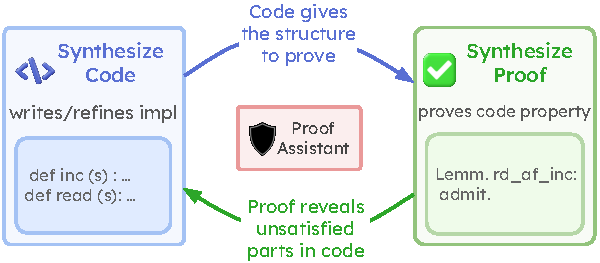
\includegraphics[width=\linewidth]{figures/img_intro.pdf}
\caption{\small Code and proof advance jointly and incrementally with IDS; the proof assistant grades each partial step. 
% \ion{I think that we need some names for the two boxes. It would make the explanation easier.}
% \mohsen{This figure is confusing. Do we need it?} \ion{I really think we need a figure. Please suggest a better one. Just draw it on a piece of paper and send out the picture.}
}
\label{fig:ids-intro}
\vspace{-0.8\baselineskip}
\end{wrapfigure}
% 
Our key insight is to synthesize both the implementation and its proof \textit{jointly and incrementally} (\cref{fig:ids-intro}), while learning from failures at each step to guide the search toward promising solutions and away from dead ends. As detailed in \cref{sec:background}, every implementation decision (e.g., adding a data structure or modifying control flow) is paired with a corresponding proof update (e.g., adding new constraints or splitting lemmas).
% As we show in \cref{sec:background}, in our approach, for each implementation decision (adding a data structure, modifying control flow, etc.), the agent correspondingly updates the proof (adding new constraints, splitting lemmas, etc.).

IDS offers two benefits: (1) each individual joint step is considerably simpler to \textit{prove}, decreasing the complexity of proof generation, and (2) the intermediate \textit{partial} proofs can be verified with a formal checker to assess the viability of the current design. A negative result rules out a dead-end implementation path before further work is wasted and serves as a counterexample to improve the design going forward.
% to report on the feasibility of getting to a correct implementation given the prior implementation decision; a \textit{no} rules out a dead-end search strategy before further work is wasted, and is provided to the agent as a counter-example to improve the strategy going forward. 
This is akin to ``chain-of-thought''~\cite{chain-of-thought},
except that the intermediate states are formally encoded and verified. %checkable for correctness. 
% \ion{The next sentence is confusing. What does extracted mean? compiled? If yes remove it, just say it is benchmarked. Also what does it mean for "proof to close"?} 
Beyond correctness, this iterative loop also optimizes performance: as soon as a candidate's implementation is complete, it is benchmarked on a distributed testbed; the performance measurements then further guide the search toward efficient implementations.
% Performance flows through the same loop: as soon as a candidate's implementation is complete, 
% it is benchmarked on a distributed testbed; the performance measurements then further steer the search towards efficient implementations.

% When deductive synthesis stalls, IDS employs an inductive feedback loop in the spirit of counter-example guided search~\cite{cegis,sketch,clarke2000counterexample}: an LLM agent analyzes previously failed strategies and pivots to more promising ones, such as proposing helper lemmas for stuck proofs.

% Our key idea is to synthesize the implementation and its machine-checkable proof \emph{jointly and incrementally} and to \emph{learn} using failures at each step as feedback to quickly steer the search toward promising strategies, away from dead ends.
%from failed attempts \ion{at each step} to \ion{quickly} steer the search toward promising strategies \ion{and thus avoid wasting computation in unpromissing directions}.
% 
% \green{An LLM agent incrementally develops a partial solution  that can have implementation placeholders with assumed specifications in the deductive-synthesis tradition~\cite{manna-waldinger,manna2006synthesis}). The proof that the partial implementation satisfies its specification can be tentatively constructed before the next steps prove that the placeholders satisfy their assumed specifications.
% 
% \ion{The rest of this paragraph doesn't say clearly why joint synthesis works. We need an explanation that can be understood by people who have never done formal spec/verification.}
% Unfilled work is staged as named placeholders (\texttt{Admitted} lemmas and stub bodies, in the deductive-synthesis tradition~\cite{manna-waldinger,manna2006synthesis}). 
% At every step the agent asks the type-checker whether the current partial implementation and proof can still extend to a complete pair; a \emph{no} rules out a dead-end design before further work is committed.}
% When deductive synthesis stalls, IDS employs an inductive feedback loop in the spirit of counter-example guided search~\cite{cegis,sketch,clarke2000counterexample}: an LLM agent analyzes previously failed strategies and pivots to more promising ones, such as proposing helper lemmas for stuck proofs.
% 
% Performance flows through the same loop: as soon as a candidate's implementation is complete, 
% it is extracted to executable code and benchmarked on a distributed testbed, even before its proof closes; the throughput then steers the search towards efficient implementations.
% so correctness and performance are co-optimized rather than sequenced.
% Note: correctness is optimized


% We apply LLM agents to synthesize the implementation and its proof \emph{jointly and incrementally}, in the deductive-synthesis tradition~\cite{manna-waldinger,manna2006synthesis}). 
% We use the proof assistant as a continuous oracle to check partial as well as complete candidates.
% Further we apply LLM agents to \emph{learn from failed proof strategies} and propose promising ones, in the inductive-synthesis tradition~\cite{cegis,sketch,clarke2000counterexample}. Incomplete lemmas and stub bodies are represented as named placeholders (\texttt{Admitted}), and at every step, the agent asks the type-checker whether the current partial pair can still extend to a complete proof; a \emph{yes} keeps a promising design alive, a \emph{no} drives exploration elsewhere.
% %  retrying with a new strategy.
% Performance flows through the same iterative process: 
% candidates are extracted to executable code, benchmarked on a distributed testbed, and their throughput is fed back as an additional signal towards efficient implementations.

% A pool of parallel \emph{Deductive Synthesis Agents} (DSAs) co-evolves implementation and proof under a \coq{} verification oracle. When a DSA stalls, an \emph{Inductive Synthesis Agent} (ISA) diagnoses the failure and responds: proposing helper lemmas for stuck proofs, or pivoting the design strategy for dead-end approaches.
%Before a candidate is accepted, a coordinator-side audit step verifies the proof is non-vacuous (e.g., that the specification was not modified and the implementation is non-trivial).

We instantiate \sys as a multi-agent system (\cref{sec:design}), and we evaluate \sys{} on 7 distributed key-value-store consistency specifications: Chapar's published causal-consistency spec~\cite{chapar} plus six new \emph{\sys{} suite} specs we release with the system (\cref{app:suite}). \sys{} produces a complete verified implementation on all 7 in about $6.8$ hours and \$$106$ per spec on average, with no human intervention or fine-tuning. On the two specs our vanilla agent baseline completed, \sys{} runs $1.6\times$ faster and $17\%$ cheaper. The discovered implementations match or beat hand-written expert references on every spec and reach up to $3\times$ the throughput of Chapar's published vector-clock reference, a margin we attribute to a design-space search broader than what manual proof allows.

As a general prover, \sys{} achieves state-of-the-art performance on four cross-language verification benchmarks (DafnyBench~\cite{dafnybench}, miniCodeProps~\cite{minicodeprops}, Verus-Bench~\cite{autoverus}, CoqStoq~\cite{rango}), beating agentic baselines that share its prompt and underlying model by $+10\%$ to $+51\%$. On three further code-and-proof synthesis benchmarks, \sys{} again leads: $176/189$ on VERINA~\cite{verina} (prior $38/189$), $65/77$ on AlgoVeri~\cite{algoveri} (prior $31/77$), and a perfect $62/62$ on CloverBench~\cite{clover}.

% \noindent In summary, we make the following contributions in this work:
% \begin{itemize}[leftmargin=*,nosep]
% \item \textbf{Inductive Deductive Synthesis (IDS):} a general technique combining incremental joint synthesis under a type-checker oracle (deductive) 
% with failure-driven improvement of the search strategy (inductive). 
% \ion{"implementation"? not sure what "strategy" means here} 
% \mohsen{search strategy for both the implementation and the proof.}
% \item \textbf{\sys{} system:} the first agentic LLM system to autonomously generate real-world distributed systems with end-to-end formal correctness guarantees.
% \item \textbf{\sys{} suite:} six \coq{} consistency specifications for distributed key-value stores, released for future verification/synthesis projects.
% \item 
% \ion{This is confusing. Maybe "\textbf{Couple performance with correctness:} use a real-world testbed to evaluate each correct implementation and steer the search toward efficient implementations."} 
% \mohsen{Agreed. This item seems odd. I think it is better to incorporate it with the first item IDS}
% \textbf{Performance in the loop:} throughput from a distributed-testbed steers the search to synthesize efficient implementations.
% % , so the loop co-optimizes correctness and performance.
% % Note: correctness is not optimized.
% \end{itemize}


\noindent In summary, we make the following contributions in this work:
\begin{itemize}[leftmargin=*,nosep]
\item \textbf{Inductive Deductive Synthesis (IDS):} the first general technique for jointly synthesizing code and machine-checked proof under a partial-proof oracle, with feedback from failures and performance benchmarks in the same loop.
\item \textbf{IDS-based multi-agent system:} the first agentic system to autonomously generate \textit{verified} distributed systems. Solves $7/7$ consistency specifications where SOTA agents (GPT-5.4, Opus 4.6) solve only $2/7$, with up to $3\times$ the throughput of published verified systems.
\item \textbf{\sys{} suite:} six new \coq{} specifications for distributed key-value-store consistency models, released as an open benchmark for verified-synthesis research.
\end{itemize}








\section{Related Work}
\label{sec:related}

% Producing certified code with an LLM involves three ?: an implementation, a specification of its guarantees, and a machine-checked proof that the implementation satisfies the specification. We position \sys{} against three lines of work that have each addressed one of these in isolation.
Verified code generation with an LLM has three components: (1) a specification of desired guarantees, (2) an implementation, and (3) a machine-checkable proof that the implementation satisfies the specification. Prior work falls into four threads: three each address one component (specification generation, program generation with an evaluator, automated proof generation), and verified synthesis attempts (2) and (3) jointly. \sys{} pursues this last class on distributed-systems specifications.

\textbf{Specification generation. \ }
A complementary line uses LLMs to recover formal specifications from code or intent~\cite{nl2postcond,autospec};
Clover~\cite{clover} generates formal annotations from natural language specifications, and then checks the consistency of code with the formal and natural specifications of Dafny benchmarks.
\sys{} takes such specifications as input rather than producing them.


% \paragraph{LLM agents and program discovery.}
\textbf{Program generation with an evaluator. \ }
% 
A separate strand of work treats program construction as search guided by evaluator feedback. 
Coding agents get feedback from given or self-generated tests~\cite{swe-agent,reflexion},
or from communication with other specialized agents~\cite{metagpt,chatdev,autogen}.
% and multi-agent systems extend this with role specialization
% 
Algorithmic discovery systems use a scoring function to drive evolution~\cite{funsearch,alphaevolve} or deep reinforcement learning~\cite{alphadev}. 
% 
\sys{} shares the evaluator-guided search scheme;
however, instead of tests or scores, it uses a proof assistant.
In contrast to sampled signals (tests over traces, specific inputs, or estimated scores),
type-checked proofs guarantee correctness on all inputs.
% accepted outputs are guaranteed on \emph{all} inputs.
% type-checking 
% The proof checker scores partial as well as complete candidates, and 


% \paragraph{Automated proof generation.}
\textbf{Automated proof generation. \ }
Most prior LLM-for-verification work fixes the implementation and specification, asking the model only for the proof.
For SMT-backed languages such as Dafny~\cite{dafny} and Verus~\cite{verus}, recent systems synthesize the loop invariants and assertions a verifier needs, either via compiler-feedback loops~\cite{autoverus} or targeted invariant generation~\cite{laurel}.
% 
For tactic-driven assistants such as Lean~\cite{lean} and \coq{}~\cite{coq}, prover systems have been trained on databases of prior formal proofs~\cite{coqgym}, natural-language proofs~\cite{wang2024theoremllama}, and conjectured theorems~\cite{dong2025stp}.
Approaches differ in scope: some generate full proofs in one pass~\cite{deepseek-prover-v2,kimina-prover,baldur}; others decompose the proof into sub-goals~\cite{li2026goedel,zhao2024subgoalxl,dsp}; tactic-level methods iteratively predict and repair the next proof step from the current proof state and verifier feedback~\cite{hubert2025olympiad,leandojo,copra,apollo,ruida2025ma}.
\sys{} differs by jointly generating the implementation and proof, and further optimizing performance.


% \paragraph{Verified synthesis from specifications.}
\textbf{Verified synthesis. \ }
The long-standing goal of producing a program and its correctness proof from a specification alone goes back to deductive synthesis~\cite{manna-waldinger,synquid} and counterexample-guided inductive synthesis~\cite{sketch,cegis}, but the inference rules and candidate-search space confined results to small individual functions.
% \sys{} is showing that these barriers can be broken in the LLM era.
% Verified-code-generation in the LLM era inherit that scope:
The LLM era rekindles this dream.
%  though significant challenges persist.
VERINA~\cite{verina} provides a benchmark to evaluate specification, code, and proof generation, evaluates existing tools, and underscores significant challenges for automatic provers.
Recent LLM-driven verified-synthesis work targets SMT-backed languages: AlphaVerus~\cite{alphaverus} bootstraps verified Verus code via self-improving translation, scaling to function-level tasks.
%
At the other extreme,
% In the past decade,
hand-built verified distributed systems, such as IronFleet's Paxos-replicated state machines~\cite{ironfleet}, Verdi's Raft~\cite{verdi}, FSCQ's crash-safe file system~\cite{fscq}, Anvil's verified Kubernetes controllers~\cite{anvil}, Chapar's causally-consistent KV stores~\cite{chapar}, and Iris-based concurrent and distributed verification~\cite{iris,grove,perennial} demonstrate that machine-checkable guarantees \emph{are} achievable at systems scale, but at months to years of expert proof effort.
% not implementation, dominating the cost.
% \sys{} shows that synthesis and certification may not mean small scale or time-consuming anymore.
\sys{} shows that verified synthesis need not be small-scale or slow: it automatically generates implementations and their machine-checkable correctness proofs for distributed key-value stores in hours rather than months.

% \paragraph{Limitations. \ }
% \sys{}' guarantees are conditional on the input specification (a formal \coq{} \texttt{Module Type}; we do not synthesize specs); we evaluate on distributed key-value-store consistency only, with generality to other domains conjectured; and \sys{} can fail on the hardest cases ($2$-of-$3$ pass rate on \sys{} suite CC). \cref{app:limitations-impacts} has full discussion.





% ===== PRIOR VERSION (commented out for reference) =====
% \section{Related Work}
% \label{sec:related}
%
% \ak{this is very overwhelming right now, cites so many different things. I feel like a good related work lays out some of the key existing points in the space, and largely helps the reader position our work with respect to them, whereas right now it reads more as focused on just listing points. }
%
% \paragraph{Automated verification.}
% Given an implementation and a specification, automated verification seeks to discharge the resulting proof obligations with minimal human effort.
% Two families of tools define the landscape.
% %
% \emph{Automated theorem provers~(ATP)} back languages such as Dafny~\cite{dafny} and Verus~\cite{verus}: an SMT solver handles most reasoning while the user supplies proof hints---loop invariants, assertions, and ghost code.
% Recent LLM-based methods generate these hints automatically.
% For Verus, AutoVerus~\cite{autoverus} uses compiler-feedback loops, AlphaVerus~\cite{alphaverus} bootstraps proofs via self-improving translation, VeruSyn~\cite{verusyn} scales through synthetic training data, RAG-Verus~\cite{rag-verus} adds retrieval augmentation, and VeriStruct~\cite{veristruct} targets data-structure modules.
% For Dafny, DafnyPro~\cite{dafnypro}, Atlas~\cite{atlas}, dafny-annotator~\cite{dafny-annotator}, Laurel~\cite{laurel}, and Reform~\cite{reform} attack invariant and assertion synthesis.
% %
% \emph{Interactive theorem provers~(ITP)}---Coq~\cite{coq}, Lean~\cite{lean}---require explicit tactic proofs but expose richer, step-level feedback to LLMs.
% Approaches span reinforcement learning and expert iteration on tactic signals~\cite{alphaproof, deepseek-prover-v1, deepseek-prover-v15, deepseek-prover-v2, goedel-prover, goedel-prover-v2, kimina-prover, seed-prover, leanabell-v2, stp, hypertree, baldur, llemma, gptf, pact, dsp}, in-context error-feedback loops~\cite{copra, leanagent, apollo, lean-copilot, palm-proofs, coqpilot, lego-prover}, retrieval-augmented tactic prediction~\cite{rango, graph2tac, tactician, proverbot9001, coqgym, passport, leandojo}, and classical-prover bridges~\cite{sledgehammer, coqhammer, thor, diva}.
% %
% All of these methods take the theorem statement as given; \sys{} instead discovers the implementation and its correctness proof jointly.
%
% \paragraph{Verified code synthesis.}
% Classical deductive synthesis---from Manna and Waldinger~\cite{manna-waldinger} through refinement calculi~\cite{morgan-refinement}, type-directed search~\cite{synquid}, sketching and CEGIS~\cite{sketch, cegis}, and tactic-based extraction in NuPRL and KIDS~\cite{nuprl, kids}---automates the derivation of correct-by-construction code from specifications, but the underlying heuristics have not scaled beyond function-level problems.
% On the LLM side, coding agents close their feedback loop on tests or self-critique~\cite{swe-agent, agentless, swebench, openhands, self-refine, reflexion}, and discovery-with-evaluator systems run evolutionary or RL search against scoring functions~\cite{funsearch, alphaevolve, alphadev, alphacode, skydiscover2026}; neither family produces formal correctness guarantees---their outputs are compile-checked, tested, or scored, but never proven correct on unseen inputs~\cite{vibe-reasoning, vibe-safe}.
% Among the few works that couple code generation with formal verification,
% Clover~\cite{clover} generates and consistency-checks (code, specification, annotation) triples in Dafny,
% and Dafny-Synthesis~\cite{dafny-synthesis} targets AI-assisted synthesis of verified Dafny methods on 50 problems.
% The VERINA benchmark~\cite{verina} evaluates the full verifiable-code-generation pipeline---code generation, specification generation, and proof generation---in Lean on 189 human-validated tasks; its comparison (Table~1 of~\cite{verina}) shows that very few existing systems address all three tasks.
% Hand-proved verified systems---Paxos in Dafny~\cite{ironfleet}, Raft in Coq~\cite{verdi}, causally consistent key-value stores in Coq~\cite{chapar}, crash-safe file systems~\cite{fscq}, and systems in Verus~\cite{anvil, verismo} and Iris~\cite{grove, iris}---demonstrate that end-to-end machine-checkable correctness is achievable, but at months to person-years of manual effort per system.
% \sys{} combines the automation goal of synthesis with the fidelity of these verified systems: an LLM agent driven by the proof assistant itself generates the (implementation, theorem, proof) triple end-to-end at systems scale.
%
% \paragraph{Specification generation.}
% A prerequisite to both verification and synthesis is a formal specification.
% Recent work uses LLMs to bridge the gap between informal intent and formal contracts.
% nl2postcond~\cite{nl2postcond} generates postconditions from natural-language function descriptions,
% AutoSpec~\cite{autospec} combines static analysis with LLM queries and program verification to infer specifications from existing code,
% and SpecGen~\cite{specgen} generates formal program specifications via LLMs.
% These efforts target specification \emph{in isolation}: given code or documentation, produce the spec.
% \sys{} addresses a complementary problem---given a specification, synthesise the implementation and its machine-checked proof---and thus consumes rather than produces specifications.
% ===== END PRIOR VERSION =====

\section{Background and Overview}
\label{sec:background}

We begin with a short introduction to formal verification.
A formally verified system has three pieces. The \emph{specification} is a precise mathematical statement of correctness; the \emph{implementation} is the code that runs; and the \emph{proof} is a machine-checkable argument that, on every input, the implementation matches the specification. Historically, humans wrote all three; \sys{} takes a human-written spec and automatically produces both implementation and proof, using LLM agents driven by the proof assistant \coq{}~\cite{coq}. We show a simple example: a \emph{counter}, a state machine with two operations (\texttt{inc} to increment the count and \texttt{read} to return it) starting from an initial state \texttt{init}.

\providecolor{specbg}{HTML}{F7F8FA}
\providecolor{specrule}{HTML}{C8CDD3}
\providecolor{speckwd}{HTML}{1F4E79}
\providecolor{partialhi}{HTML}{FFF3CD}
\providecolor{completehi}{HTML}{D4EDDA}

\begin{figure}[tb]
\centering
\lstset{
  language=Coq,
  basicstyle=\ttfamily\scriptsize,
  keywordstyle=\bfseries\color{speckwd},
  showstringspaces=false,
  columns=fullflexible,
  breaklines=true,
  numbers=none,
  frame=single,
  framerule=0.3pt,
  framesep=3pt,
  rulecolor=\color{specrule},
  xleftmargin=4pt,
  xrightmargin=2pt,
  backgroundcolor=\color{specbg},
  aboveskip=0pt,
  belowskip=0pt,
}
\begin{minipage}[t]{0.32\textwidth}
\centering
\textbf{Specification}\\[2pt]
\begin{lstlisting}
Module Type CounterSpec.

  Parameter t    : Type.
  Parameter init : t.
  Parameter inc  : t -> t.
  Parameter read : t -> nat.

  Axiom read_init :
    read init = 0.

  Axiom read_inc :
    forall s,
    read (inc s) =
      S (read s).

End CounterSpec.
\end{lstlisting}
\end{minipage}\hfill
\begin{minipage}[t]{0.32\textwidth}
\centering
\textbf{Partial impl.\ \& proof}\\[2pt]
\begin{lstlisting}
Definition t := list unit.
Definition init : t := nil.
\end{lstlisting}
\begin{lstlisting}[backgroundcolor=\color{partialhi}]
Definition inc (s : t) : t.
Admitted.
\end{lstlisting}
\begin{lstlisting}
Definition read (s : t) :=
  length s.

Theorem read_init :
  read init = 0.
Proof. reflexivity. Qed.
Theorem read_inc :
  forall s,
  read (inc s) = S (read s).
\end{lstlisting}
\begin{lstlisting}[backgroundcolor=\color{partialhi}]
Admitted.
\end{lstlisting}
\end{minipage}\hfill
\begin{minipage}[t]{0.32\textwidth}
\centering
\textbf{Complete impl.\ \& proof}\\[2pt]
\begin{lstlisting}
Definition t := list unit.
Definition init : t := nil.
\end{lstlisting}
\begin{lstlisting}[backgroundcolor=\color{completehi}]
Definition inc (s : t) :=  tt::s.
\end{lstlisting}
\begin{lstlisting}
Definition read (s : t) :=
  length s.
Theorem read_init :
  read init = 0.
Proof. reflexivity. Qed.
Theorem read_inc :
  forall s,
  read (inc s) = S (read s).
\end{lstlisting}
\begin{lstlisting}[backgroundcolor=\color{completehi}]
Proof. intros s. unfold read, inc.
  simpl. reflexivity. Qed.
\end{lstlisting}
\end{minipage}
\caption{Counter \textit{specification} (left), \textit{partial} synthesis (center, yellow = \texttt{Admitted}), and \textit{complete} synthesis (right, green = filled in). \coq{} accepts both files.}
\label{fig:counter-listing}
\end{figure}


Figure~\ref{fig:counter-listing} shows the counter's \textit{specification} (left), a \textit{partial synthesis} (center), and a \textit{complete synthesis} (right). The spec states two properties, or ``axioms,'' about \texttt{init}, \texttt{inc}, and \texttt{read}: reading the initial state returns zero, and reading after an increment returns one more than reading before. In the partial synthesis, \texttt{inc}'s body and the \texttt{read\_inc} theorem are deferred via \texttt{Admitted} (a placeholder for unfinished work), but \coq{} still accepts the file: the chosen representation (a list whose length encodes the count) is consistent with the work so far. The complete synthesis fills in the deferred pieces.
The representation is a free choice; any state satisfying the axioms works, though \texttt{nat} (natural numbers) is more efficient.


\textbf{\coq{}'s type-checker as an oracle, including for partial work. \ }
\coq{}'s checker \textit{accepts} a declaration/proof if and only if it satisfies its stated type/proposition, and rejects with a precise diagnostic otherwise. There are no false positives or false negatives, in contrast to tests (only the inputs tried), static analysis (over-approximate), or LLM-as-judge (guesses). The verdict also extends to \emph{partial} code, as the center column of Figure~\ref{fig:counter-listing} illustrates: unproven obligations are stated as \emph{deferred holes} (\texttt{Admitted} lemmas or stub function bodies), and the file still type-checks.
(\cref{app:progression} walks a longer \texttt{all\_less\_than} example through this progression.)
\sys{} leverages the type-checker as an oracle to drive a \emph{deductive synthesis}~\cite{manna-waldinger}: at every step, the agent extends the partial implementation and proof, then asks \coq{} whether the partial state still type-checks. A yes keeps the design on track; a no rules it out before further work is committed. \aknew{If progress stalls (measured by the number of partial proofs left empty), IDS reverts to an earlier state.}


\textbf{From counter to distributed stores. \ }
\sys{} applies this loop at scale.
For distributed systems, the specification grows from simple axioms to conditions over executions involving messages, clients, replicas, and failures.
For example, \texttt{read\_inc} in a distributed setting becomes read-your-writes: a client that increments then reads must observe its own increments.
The implementation grows from a few-line module to a multi-replica protocol with larger state, multiple message types, and handlers.
For example, a replica can no longer store one \texttt{nat}; it must keep a vector with one entry per client, tracking the increments received from that client. On a request carrying the client's increment count, the replica can then tell whether it is up-to-date enough to serve, providing read-your-writes.
The proof grows from simple tactics to an inductive simulation argument (an induction linking implementation and spec states) with dozens of helper lemmas.

Such implementations span a large, subtle design space with widely varying performance, explored by decades of research. \cref{sec:design} describes the agent that drives this process, \cref{app:suite} gives the full specifications, and \cref{sec:eval} reports results.


% ===== PRIOR (BULLET) DRAFT - kept for reference =====

% \shubham{Simple example where we show proof implementation, and how this goes to do the synthesis and proof}

% \accheng{I would make sure to be clear where AI can fit into this process. What was manual before? What needs to be manual now?}

% \mohsen{If you have oracle, then why do we need LLM?}
% \mohsen{Specification, agent generate proof. understood, but why challenges, manually. Why Vibe proof is the right tool.}
% \mohsen{Not clear: oracle, previous work using Lean, challenges for distributed computing}
% \mohsen{Example}

% \paragraph{Specification, implementation, and proof.}
% \begin{itemize}
%   \item \emph{Specification}: a precise mathematical statement of what correctness means (e.g., ``all clients see operations in causal order'').
%   \item \emph{Implementation}: concrete types and functions that fit the spec's module interface (e.g., a \texttt{get}/\texttt{put} key-value store with vector clocks).
%   \item \emph{Proof}: a machine-checked argument that the implementation satisfies the spec (e.g., a simulation between concrete state and spec state).
%   \item In a \emph{modular framework} (such as Coq's \texttt{Module Type}), the spec and the module interface are \emph{fixed inputs}; the implementation and proof are the \emph{creative outputs} to produce.
% \end{itemize}

% \paragraph{Deductive synthesis.}
% \begin{itemize}
%   \item \emph{Joint construction}: produce implementation and proof together against a fixed spec~\cite{manna-waldinger}.
%   \item \emph{Stepwise refinement}: advance one step at a time, with the type-checker as the gate~\cite{morgan-refinement}.
%   \item \emph{Deferred holes}: state a sub-goal as a named placeholder (e.g., an \texttt{Admitted} lemma or a stub) and discharge it later, in the Sketch tradition~\cite{sketch}.
%   \item \emph{Structural coupling}: data structures determine which invariants hold, which determine which lemmas are provable; one design change can invalidate the entire proof tree.
%   \item \emph{Sequential human practice}: pick a design, prove for months, rarely revisit; performant designs often resist proof, and proof-friendly designs are often slow.
%   \item \emph{Example flow}: from a causal-consistency spec, choose vector clocks for state; write \texttt{get}/\texttt{put} method bodies; state and discharge non-simulation obligations (initialisation, preservation); finally prove a simulation lemma. The type-checker gates each step; \texttt{Admitted} holes are filled later.
% \end{itemize}

% \paragraph{Proof assistants as perfect verification oracles.}
% \begin{itemize}
%   \item A proof assistant (Coq, Lean, Dafny, Verus) is an environment whose kernel checks each definition and lemma against the type theory as you write it.
%   \item The verdict is exact: \emph{accept} iff mathematically correct, \emph{reject} with a precise diagnostic. No false positives, no false negatives, in contrast to tests (only the inputs tried), static analysis (over-approximate), or LLM-as-judge (guesses).
%   \item The oracle also works on \emph{partial} code: an \texttt{Admitted} axiom or stub stands in for an unproven sub-goal, and the rest of the file still type-checks. An agent can therefore tell ``this branch is on track'' from ``this branch is a dead end'' without committing to a full proof.
%   \item Yet the oracle scores candidates but does not propose them: the design, the next sub-lemma to factor, and when to abandon a path are open. \cref{sec:design} describes the agent that closes that loop.
% \end{itemize}

% \input{figures/dist-counter}


\section{\sys{} Agentic Architecture}
\label{sec:design}

\begin{figure}[t]
   \centering
   \noindent\hspace*{-6pt}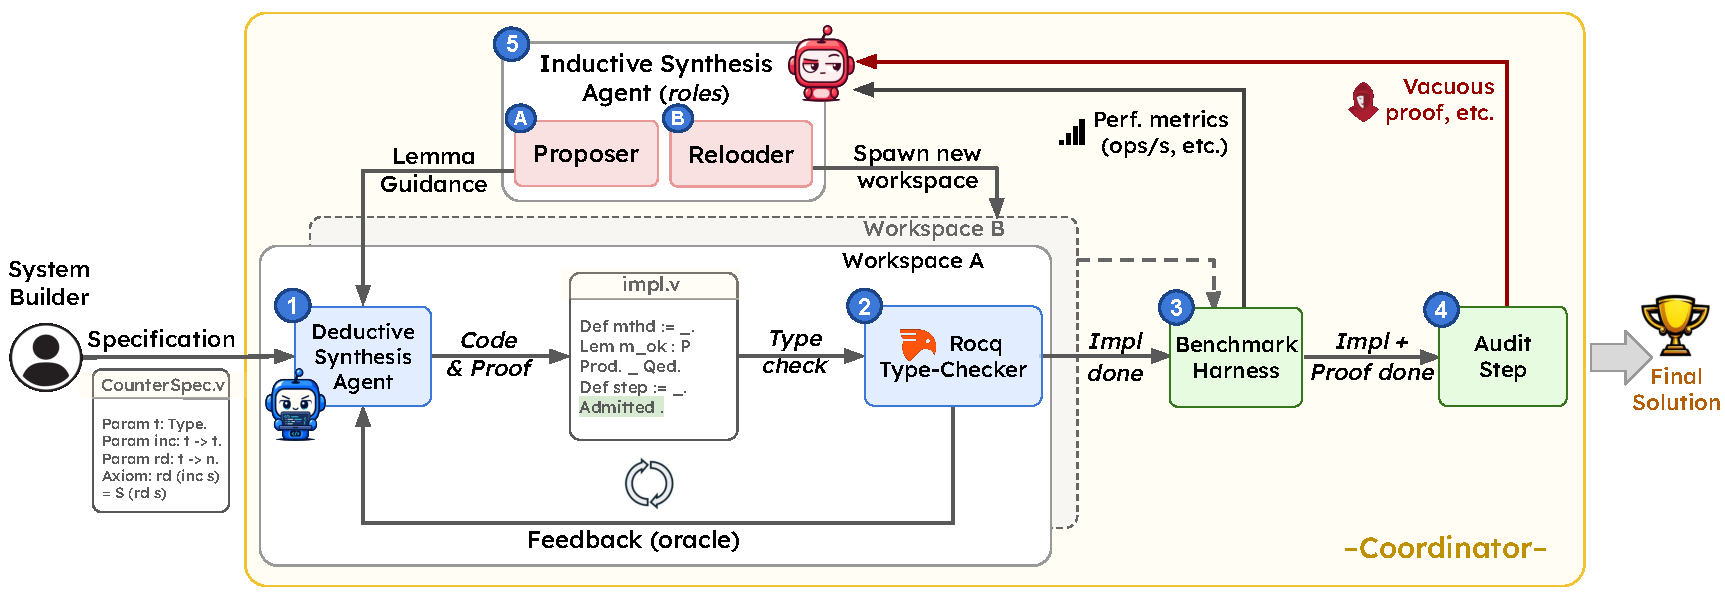
\includegraphics[width=\dimexpr\linewidth+12pt\relax]{figures/OVERVIEW_final.pdf}\hspace*{-6pt}
   \caption{\sys{}' agentic architecture; code and proof advance jointly throughout. A coordinator runs parallel \fignum{1} Deductive Synthesis Agents (DSAs); each step is graded by \fignum{2} \coq{}'s type-checker, completed implementations are \fignum{3} benchmarked, and closed proofs are \fignum{4} audited for non-vacuity. On failure, the \fignum{5} Inductive Synthesis Agent (ISA) intervenes: \fignum{A} \emph{proposer} adds helper lemmas on tactical stalls; \fignum{B} \emph{reloader} respawns a DSA with a fresh design on strategic dead-ends.
% \mohsen{Can we add 5 and 6 for proposer and reloader as well?} \shubham{Addressed: \fignum{5} for ISA, \fignum{A} for proposer, \fignum{B} for reloader (matching the figure's 5 / A / B labels).}
}
   % \mohsen{Strategist Agent -> Inductive Synthesis Agent}}
   \label{fig:architecture}
\end{figure}
% \shu{can we even make the specification and the code generation block larger? Audit step is done by an agent right? should we have a role there?}
% \mert{there is a lot of unused empty space, perhaps the figure can be arranged to make the code and writings look larger?}
% \mohsen{The text needs to be larger.}

% \accheng{can we try to structure the text to be more readable? the paragraphs are too dense right now and hard to get what the main takeaways are. I would try to highlight insights, key design decisions, etc. Right now, it reads more like a description of an implementation}

\textbf{Overview. \ }
%
We now describe how we realize IDS as an agentic architecture (\cref{fig:architecture}). Given a system interface and property specifications, the framework orchestrates multiple LLM agents guided by verification and performance feedback to generate an efficient, mechanically-checked implementation. This architecture relies on a powerful synergy: deductive synthesis constructs the code and proof under a given strategy, while inductive synthesis discovers better strategies from failed attempts.
% This paper realizes IDS as an agentic certified synthesizer.
% 
% Our framework takes as input the signature of a distributed key-value-store implementation and the specification of its properties.
% It then uses multiple LLM agents, with a proof assistant providing verification feedback,
% and a benchmark harness providing performance feedback,
% to generate an efficient implementation
% paired with a mechanically-checked proof that it satisfies the specification.
% Deductive and inductive synthesis form a powerful combination:
% % deductive synthesis produces rigorous proofs,
% % and inductive synthesis discovers effective proof strategies.
% % Deductive and inductive synthesis combine naturally in IDS: 
% given a strategy, deductive synthesis constructs an implementation and a machine-checked proof; 
% given failed attempts, inductive synthesis discovers more effective strategies.

% Inspired by deductive synthesis~\cite{manna-waldinger,manna2006synthesis}, \sys{} introduces Deductive Synthesis Agents (DSAs, \fignum{1}) to incrementally synthesize implementations from specifications. Guided by a strategy, a DSA decomposes a component into sub-components. It inserts placeholders for these sub-components to construct the parent implementation, simultaneously decomposing the parent specification into corresponding sub-specifications. This step leverages both the specification's structure (\ie a specification composed of multiple methods naturally splits into separate specifications for each method) and the LLM's knowledge of decomposition patterns. Assuming the sub-components satisfy their sub-specifications, the DSA constructs the proof of correctness for the parent component. This recursive process repeats until the search tree reaches trivial sub-components and sub-specifications. The agent applies a similar approach to decompose lemmas into helper lemmas. At every step, it uses the \coq{} type-checker (\fignum{2}) to verify the correctness of both complete and partial proofs.

Inspired by deductive synthesis~\cite{manna-waldinger,manna2006synthesis}, \sys{} introduces Deductive Synthesis Agents (DSAs, \fignum{1}) to incrementally synthesize implementations from specifications. Guided by a strategy, a DSA recursively decomposes a component and its specification into sub-components using placeholders. 
% Leveraging the LLM's structural knowledge, 
The DSA constructs proofs assuming these sub-components are correct, repeating this process down to trivial elements. The \coq{} type-checker (\fignum{2}) continuously verifies both complete and partial proofs throughout this decomposition.

% Inspired by deductive synthesis~\cite{manna-waldinger,manna2006synthesis},
% \sys{} introduces Deductive Synthesis Agents (DSAs, \fignum{1})
% that incrementally synthesize the implementation from the specification.
% Given a strategy, 
% a DSA decomposes the synthesis of a component into the synthesis of sub-components.
% It sets placeholders for implementations of sub-components
% and constructs an implementation of the component using the sub-components.
% It further
% decomposes the specification of the component into sub-specifications for the sub-components.
% It draws on both the specification's structure (\ie a specification composed of multiple methods naturally splits into separate specifications for each method) and the LLM's knowledge of decomposition patterns.
% Assuming sub-components satisfy their sub-specifications,
% it constructs the proof of correctness for the component.
% It then repeats the process for sub-components.
% The process terminates when the search tree reaches trivial sub-components and sub-specifications.
% It takes a similar approach in decomposing lemmas into helper lemmas.
% It uses the type-checker of \coq{} (\fignum{2}) to check the correctness of complete as well as partial proofs at each step.
% decomposed specifications of its sub-components.
% \shu{step 3 is missing, overview is way, way too long... it is very hard to parse, can we make it shorter?}
% DSA proves effective when driven the right path.


% A DSA is effective when guided by a good search strategy\shu{is strategy defined somewhere? what is strategy? is it code?}, such as introducing the right ghost state
% (an auxiliary variable that is added to captures an invariant).
% However, with a dead-end strategy, a DSA may get stuck taking steps without closing the proof.
%
% \accheng{do you already explain what CEGIS is before? I wouldn't assume reviewers are familiar} \shubham{Could name the counterexample at the inner DSA level as the structured \coq{} error trace (\cref{app:feedback}); FB ablation in \cref{sec:eval-ablations} confirms the trace, not just a binary verdict, carries the signal.}
% In the spirit of inductive synthesis, 
% Inspired by inductive synthesis~\cite{cegis,sketch,clarke2000counterexample}, \sys{} introduces an Inductive Synthesis Agent (ISA, \fignum{5}) that learns from failed strategies and proposes more promising ones. 
% It is given feedback
% when a DSA stalls at a proof attempt and 
% when the performance is evaluated.
% The ISA plays two roles, \emph{proposer} (tactical, \fignum{A}) and \emph{reloader} (strategic, \fignum{B}). \shu{what is tactical and strategic?}
% A DSA is effective when guided by a sound search strategy, which represents a high-level design or proof approach such as introducing the right ghost state (an auxiliary variable used to capture an invariant). However, under a dead-end strategy, a DSA may get stuck taking steps without closing the proof. 
% Inspired by inductive synthesis~\cite{cegis,sketch,clarke2000counterexample}, \sys{} introduces an Inductive Synthesis Agent (ISA, \fignum{5}) that learns from failed strategies and proposes more promising ones. The ISA receives feedback when a DSA stalls at a proof attempt and when system performance is evaluated. The ISA plays two roles: a \emph{proposer} for tactical, local adjustments to the current approach (\fignum{A}), and a \emph{reloader} for strategic, global shifts to entirely new designs (\fignum{B}).

While this deductive approach succeeds when guided by a sound search strategy (e.g., a high-level design or proof approach in the prompt), a DSA can stall under a dead-end strategy. Inspired by inductive synthesis~\cite{cegis,sketch,clarke2000counterexample}, \sys{} introduces an Inductive Synthesis Agent (ISA, \fignum{5}) that learns from failed strategies to propose more promising ones. The ISA receives feedback when a DSA stalls or yields poor performance. It then intervenes in two roles: a \emph{proposer} for tactical, local adjustments (\fignum{A}), and a \emph{reloader} for strategic, global shifts to entirely new designs (\fignum{B}).

% informed of a failed strategy
% Here the role of the counterexample is played by two negative signals to the ISA: 

\textbf{Coordinator. \ } The coordinator launches and orchestrates the DSAs and the ISA, maintaining overall system state and managing a parallel pool of workers. While DSAs can report localized errors, they cannot detect strategic dead-ends on their own. The coordinator monitors progress to identify stagnating agents, recording failed strategies and invoking the ISA to propose new ones before respawning the DSA. 
 
To ensure the synthesized system is not only correct but also performant, the coordinator benchmarks each candidate eagerly, even before its proof completes. It extracts the implementation to executable code and runs the benchmark harness (\fignum{3}, \cref{sec:eval-setup}). The measurements are fed back to the ISA so that its future strategies guide the DSA toward more efficient implementations. Once a proof closes (i.e., the proof completes with no remaining \texttt{Admitted} placeholders), the coordinator audits the result to ensure it is fully verified, non-trivial, and implements the expected interface (\fignum{4}). Finally, it returns the most efficient verified solution found within the time budget. 
% Next, we consider the DSA and ISA more closely.


% \sys{} presents a coordinator that orchestrates the DSAs and the ISA.
% \textbf{Coordinator. \ }
% The coordinator launches and orchestrates the DSAs and the ISA, and maintains state. The coordinator starts with one DSA and grows a pool of DSAs in parallel over time.
% In order to avoid the sunk-cost fallacy, the DSA reports when it is stuck with a repeating error; however, it cannot tell when it faces a strategic dead-end. Therefore, the coordinator periodically polls each DSA and tracks the number of open and finished proofs. 
% If it deems that a DSA is stagnating,
% it records the failed strategy,
% and invokes the ISA
% to either revise the strategy, or propose a new one.
% It then respawns the DSA with that strategy, or spawns an additional DSA.
 

% The coordinator benchmarks each candidate eagerly, 
% even before its proof completes.
% The coordinator extracts the implementation to executable code,
% % from Gallina to OCaml
% and runs the benchmark harness (\fignum{3}, \cref{sec:eval-setup}).
% The measurements are fed back to the ISA
% so that its future strategies
% guide the DSA toward more efficient implementations.
% % 
% % Finally, the coordinator returns the most efficient verified solution
% % that was found in the time budget.
% The coordinator
% runs the audit step (\fignum{4}) when the proof closes.
% In addition to type-checking, it checks that (i) no assumptions
% % \texttt{Axiom}/\texttt{Hypothesis}/\texttt{Parameter}/\texttt{Admitted} 
% remains in the final output, (ii) the expected interface is implemented, (iii) the implementation is non-trivial, and (iv) the proper correctness statement is included.
% % 
% Finally, it returns the most efficient verified solution
% found within the time budget.
% 
% 
% coordinator, 
% Next, we consider the DSA and ISA more closely. \shu{this is very long, some of the details in the first paragraph is about implementation right? imo we should have a shorten overview that includes all points, and dive into specific agents in subsequent paragraphs}
% in turn.

% Worker holds proof state across many turns while Meta sees only summaries -- separating context windows lets Worker stay deep without Meta drowning in tokens


% \mert{
% Overall, this multi-agent archiecture needs to be well motivated. It should not feel like this archiecture is vibe-coded, abut there is an essential need and a natural nreason behind these agentic roles. Also it is not super clear if \emph{Heartbeat} is an agent or not, the difference between the \emph{Guide} and \emph{Resetter} or \emph{Meta}.
% Why cant these be a single agent that is equipped to do multiple responsibilities given different situations for example? Context management can be a key reason, but needs to be motivated.} 
% \accheng{agree, providing some high-level motivation for the overall architecture will make it more convincing}
% \shubham{Can add a ``Why multi-agent'' opener: (a) Heartbeat is deterministic Python (not an LLM), so ``DONE'' is a kernel-level verdict not another model output; (b) Worker holds proof state across many turns while Meta sees only summaries -- separating context windows lets Worker stay deep without Meta drowning in tokens; (c) Guide/Resetter are different decision horizons (tactical vs strategic) and a single agent making both calls in one prompt empirically picks the wrong move when the failure mode is mixed.}


% % ------------------------------------------------------
% \textbf{Coordinator. \ }
% % \subsection{Monitor}
% \label{sec:design-heartbeat}
% % 
% The coordinator is a program that launches the agents, maintains state, and coordinates them. It is deterministic Python rather than an LLM, so its verdicts (a DSA is stagnating; a candidate is audit-clean) are kernel-level rather than model outputs. It starts with one DSA and grows the pool over time, with each DSA exploring a different synthesis tree in its own sandboxed workspace. 
% The DSA reports when it is stuck with a repeating error; however, it cannot tell when it faces a strategic dead-end. Therefore, the coordinator polls each DSA every $5$ minutes and tracks the number of open and finished proofs (\ie \texttt{Admitted} and \texttt{Qed} terms): if neither count has changed across $10$ consecutive polls, the DSA is flagged as stagnating, and the coordinator invokes the ISA with the previous strategies, escalating with a new ISA invocation every $20$ further polls of continued stagnation. The ISA then refines the current strategy or proposes a new one. The coordinator provides the DSA with the refined strategy, respawns it with the new one, or spawns an additional DSA in a new workspace.
% 
% The coordinator empirically evaluates not only a DSA's verified solutions but also implementations whose proof is incomplete.
% This eager evaluation helps avoid verifying an implementation that is slower than previously-known candidates.
% The coordinator extracts the implementation to executable code,
% % from Gallina to OCaml
% and runs the benchmark harness (\cref{sec:eval-setup}).
% % If the implementation is slow,
% It then passes the performance feedback to the ISA, which gives the DSA a new strategy.
% %
% When a DSA closes the proof, the coordinator runs the audit step: in addition to type-checking, it checks that the expected interface is implemented, the implementation is non-trivial, and the proper correctness statement is included. If the audit step rejects the candidate (e.g., a vacuous proof), it is sent to the ISA.
% %
% % The coordinator returns the best known solution or failure when the allocated time is over.
% The coordinator returns the best solution found, or reports failure, upon exhausting the time budget.
% 
% % \item \textbf{If Meta itself stagnates.} If Meta's interventions yield no new \texttt{Qed} across $N$ consecutive heartbeats, Heartbeat fires a one-shot Meta-Meta call: a higher-level invocation that reads Meta's prior guidance and proposes a strategy Meta has not yet tried.



\textbf{DSA: Deductive Synthesis Agent. \ }
% \subsection{DSA: Deductive Synthesis Agent}
\label{sec:design-worker}
Off-the-shelf LLMs, pretrained on a large corpus of programs and proofs, are well-equipped to guide synthesis search,
as we empirically demonstrate in \cref{sec:eval-synthesis}. To harness this capability, we design the DSA as a generic LLM coding agent operating under strict constraints: implementations must be well-typed before proving, specifications cannot be altered, final outputs must contain no unproven assumptions, and system state must remain bounded.

% Pretrained on a large corpus of programs and proofs,
% off-the-shelf LLMs are well-equipped to guide the synthesis search,
% as we empirically demonstrate in \cref{sec:eval-synthesis}.
% A DSA is a generic headless LLM coding agent (Codex, Claude Code) with the following briefings.
% % 
% \emph{Methodology.} 
% % Plan the implementation before writing code.
% The implementation should be well-typed before attempting a proof.
% The refinement relation between the states of the implementation and specification should be explicitly written and type-checked.
% % non-simulation obligations (initialisation, preservation, parametricity) are discharged before the main simulation theorem.
% % 
% \emph{Auditability.} 
% The specification shouldn't be changed.
% No assumptions
% % \texttt{Axiom}, \texttt{Hypothesis}, \texttt{Parameter}, or \texttt{Admitted} 
% should be in the final output.
% % 
% \emph{Design.}
% The declared system state should not grow unboundedly with the number of operations.
% 
% \item
% \emph{Tactical playbook.} Use the curated set of tactic patterns from interactive-proof practice (\cref{app:proof-method}).

At each node of the search tree, the agent can take the following actions to advance the synthesis: (1) define partial implementations, (2) close open proof branches, or (3) decompose complex lemmas into simpler helper lemmas. After each step, the implementation and proof are passed to \coq{}'s type-checker. If there are no errors, the state is saved, building a search tree of well-typed partial implementations and proofs. If errors occur, the agent can take the following actions: (1) repair the failed step by attempting a different approach, or (2) revert to an earlier node in the search tree.

% % The DSA is \sys's deductive-synthesis agent: 
% Given a specification, a DSA incrementally refines it into an implementation.
% % and a machine-checked proof that the implementation satisfies the specification.
% % The specification declares the interface to implement and the properties the implementation must satisfy.
% % The agent 
% In order to synthesize a component, it chooses a strategy, generates placeholders for the required sub-components, and implements the component using the sub-components.
% Accordingly, it decomposes the specification into sub-specifications for sub-components, drawing on both the spec's structure (a spec composed of multiple methods naturally splits into per-method obligations) and the LLM's knowledge of decomposition patterns.
% It then assumes that the sub-components will satisfy the sub-specifications, and
% constructs a proof that the implemented component satisfies its specification.
% In the next iterations, the agent continues to synthesize
% % implementations of the 
% sub-components that satisfy the sub-specifications.
% % Finally, the search tree culminates in trivial sub-components and sub-specifications.
% The process terminates when the search tree reaches trivial sub-components and sub-specifications.
% 
% At each node of the search tree, the agent can take the following actions.
% % each step of the search
% (1) \emph{Define}: 
% Declare, refine or extend a state or message type, or function body. Partial function definitions can be written with placeholders (\ie \texttt{admit}) which are tackled in the next steps.
% % 
% (2) \emph{Prove}:
% Close an open proof obligation (\ie replace \texttt{Admitted} with \texttt{Qed}) or extend the proof with more tactics.
% % 
% (3) \emph{Decompose}:
% State and assume helper lemmas (\ie as \texttt{Admitted}) which are tackled in the next steps. Then, use the helper lemmas to advance the proof of existing lemmas.
% % 
% After each of the above steps,
% the implementation and proof
% are passed to \coq{}'s type-checker as the oracle.
% % After each step, 
% If there are no errors,
% the state of the synthesis and the output of the oracle are logged in a file.
% % (The file further reports information such as the number of lines and \texttt{Qed}s/\texttt{Admitted}s, and the current active goal).
% Thus, a DSA's history maintains a search tree of well-typed partial implementations and proofs. 
% % The tree is the coordinator's reconstruction from the DSA's per-step snapshots; the DSA itself reasons turn-by-turn through its prompt history rather than over an explicit tree.
% % \mohsen{Above not clear.}
% % Otherwise,
% On the other hand, if there are errors,
% the agent can take the following actions.
% (1) \emph{Repair}:
% Re-attempt the failed step such as applying a different tactic.
% For example, apply induction instead of case analysis.
% (2) \emph{Revert}:
% Rewind to the state of an earlier node in the search tree.
% %
% % As we will empirically demonstrate in \cref{sec:eval-setup}.
% The implementation and proof are constructed together; a step on the implementation can invalidate the proof, and a proof obligation that the agent cannot close is evidence that the program needs to change.





% The DSA keeps extending its search tree; however, in order to avoid falling for the sunk cost, if the same error recurs three or more times, it reports the failing attempt to the coordinator. 
% % The match is semantic, judged by the agent itself rather than exact-string, so paraphrased restatements of the same issue still count.
% % 
% On the other hand, if it completes all the definitions and theorems,
% it reports the candidate solution to the coordinator.

\textbf{ISA: Inductive Synthesis Agent. \ } The DSA cannot reliably step back and pivot a failing strategy on its own. The ISA fills this gap as a stateless LLM agent that reasons over a strategy summary and proposes new approaches across two decision horizons: \begin{itemize}[leftmargin=*,nosep,topsep=2pt] 
\item \textbf{Proposer (tactical).} Triggered when the strategy is promising but the DSA is stuck on a specific proof. The proposer offers finer-grained assistance, suggesting helper lemmas and structural decompositions from a holistic view of the proof state.
\item \textbf{Reloader (strategic).} Triggered when the strategy is a dead-end or slow. Rather than allowing the DSA to endlessly apply small fixes, the reloader intervenes by respawning the DSA with an entirely new high-level design.
\end{itemize}


% \textbf{ISA: Inductive Synthesis Agent. \ }
% % \subsection{ISA: Inductive Synthesis Agent}
% \label{sec:design-roles}
% 
% The DSA cannot reliably step back and pivot a failing strategy on its own. The ISA fills this gap: a stateless LLM agent that reasons over a strategy summary, and proposes a new strategy. It plays two roles for different decision horizons:
% % (not the DSA's full proof state)
% \begin{itemize}[leftmargin=*,nosep,topsep=2pt]
% \item \textbf{Reloader (strategic).} Triggered when the strategy is a dead-end or slow. Without intervention, the DSA would keep applying small fixes to proof steps (\eg swapping one tactic for another) without questioning the larger strategy. The reloader takes a more drastic step: it kills the DSA and respawns it with a new strategy, picking a different design (\eg vector clock instead of dependency list, or per-key map instead of a global log).
% \item \textbf{Proposer (tactical).} Triggered when the strategy is promising but the DSA is stuck in the proof of a lemma; a full strategy shift might not be warranted. The proposer takes a finer-grained step: it suggests helper lemmas and a decomposition of the obligation, similar to the DSA's own decompose step but from a holistic view of the involved lemmas.
% \end{itemize}

% \shu{this entire section reads super long}
% \mohsen{Now is shorter, cut parts}






\section{Evaluation}
\label{sec:eval}

We evaluate \sys{} on 7 \coq{} specifications of distributed key-value-store consistency: Chapar's published causal-consistency spec~\cite{chapar} and 6 new \emph{\sys{} suite} specs co-developed with a formal-verification and distributed-systems expert (\cref{app:suite}). We extract synthesized implementations from Gallina to OCaml and benchmark them on a 5-VM Google Cloud cluster under a distributed runtime against hand-written expert references. For synthesis, we compare against SOTA coding agents, Codex (GPT-5.4)~\cite{codex} and Claude Code (Opus 4.6)~\cite{claude-code}, under the same prompt and budget. We answer three questions in the following subsections:
\begin{itemize}[leftmargin=*,nosep,itemsep=2pt,topsep=2pt]
\item \textbf{Q1. Does \sys{} handle hard specifications?} \sys{} succeeds on all $7$ in about $6.8$ hours and \$$106$ per spec on average (max $11$h, \$$155$), versus $2$ of $7$ each for Codex and Claude Code under the same prompt and budget (\cref{sec:eval-synthesis}).
\item \textbf{Q2. Are the synthesized implementations performant?} They match or beat every expert-implemented reference: $3\times$ throughput on Chapar's vector-clock reference, $1.4\times$ on \sys{} suite CC and monotonic reads, comparable on read-your-writes (within $20\%$), and sustained throughput on MW and RYW+MW where the reference times out (\cref{sec:eval-perf}).
\item \textbf{Q3. Which of \sys{}' design decisions drive these results?} The joint code-and-proof co-design, the ISA's proposer and reloader roles, the audit step, the \coq{} feedback to the DSA, and the performance feedback to the ISA each contribute consequentially. The DSA alone also sets a new state-of-the-art on four public proof benchmarks across four languages (\cref{sec:eval-ablations}).
\end{itemize}

\subsection{Experimental Setup}
\label{sec:eval-setup}

\textbf{Specifications. \ }
Each specification is a high-level reference implementation of a key-value store; its state type and operations define the consistency notion. \sys{} takes a specification and produces a refining implementation paired with a machine-checked proof of correctness on every input.

Chapar~\cite{chapar} provides a published causal-consistency specification (CC). The other six form the \emph{\sys{} suite} benchmark dataset that we release alongside the system (\cref{app:suite}): read-your-writes (RYW), monotonic writes (MW), monotonic reads (MR), their composition (RYW+MW), and two causal-consistency variants: \sys{} suite CC and LCC (\emph{labeled} causal consistency, where each client subscribes to a set of topic labels and sees causality enforced only on those labels). The \sys{} suite spans the space of session consistency guarantees. To the best of our knowledge, no prior benchmark provides verified \coq{} artifacts across this range.
% 
Difficulty grows in three tiers: simple (RYW, MW), specs whose proofs need many cases (MR, RYW+MW), and specs that also manage explicit dependency sets (CC, LCC).
% through specifications whose proof needs multi-case splits , to specifications that require bridging the implementation's vector clocks to the spec's explicit dependency sets (CC, LCC). 
A side-by-side summary of all seven specifications appears in \cref{app:consistency-specs}.

\textbf{Harness and metrics. \ }
Verified \coq{} implementations are extracted to OCaml (via \coq{}'s built-in extraction, an automatic compilation pass from Gallina to OCaml) and run under a distributed runtime on a 5-VM Google Cloud cluster. Each run executes $4$ parallel workers $\times$ $1{,}000$ random operations; we sweep across put rates, and run a separate scaling sweep at put rate~$=50\%$ over $N \in \{1{,}000, 2{,}000, 5{,}000, 20{,}000\}$. \cref{app:perf-harness} covers the cluster topology and toolchain.
% 
% \mohsen{We already said these in section 3. Commented.}
% A run \emph{closes} a benchmark when \coq{} accepts the proof with no \texttt{Admitted}, \texttt{Axiom}, \texttt{Hypothesis}, or \texttt{Parameter} terms, the audit step (\cref{sec:design-heartbeat}) accepts the candidate, and the extracted OCaml runs on the harness. 
Every method runs under the same per-spec wall-clock and dollar budget. Runs that exhaust either budget are considered failed runs. 
% before closing 
Each cell aggregates three independent runs, and we report pass rate 
% (closures out of three), 
(successes out of three), 
time-to-finish, dollar cost, throughput, p99 latency, peak memory, and ops-per-worker scaling, all as medians.

\textbf{Baselines. \ }
The synthesis baselines are Codex (GPT-5.4)~\cite{codex} and Claude Code (Opus 4.6)~\cite{claude-code}. Both run under the same prompt and budget as \sys{}' DSA, so the comparison isolates the agentic architecture. Codex is also \sys{}' primary backend. 
For performance comparisons, the references are the hand-written expert implementations: 
Chapar's two published references (vector-clock and list-based)~\cite{chapar}, and the expert-written reference released alongside each \sys{} suite specification, except LCC, a custom spec with no expert reference.
% 
For the cross-language evaluation, 
we adopt four public verification benchmarks (DafnyBench, Verus-Bench, miniCodeProps, CoqStoq) across the languages Dafny, Verus, Lean, and \coq{}. 
We compare against the strongest published prior tool for each benchmark.
\cref{app:benchmarks} covers three more (VERINA, AlgoVeri, CloverBench). These cross-language benchmarks target function- and algorithm-level tasks, smaller and simpler in scope than the real-world distributed systems above.

\definecolor{rowhl}{HTML}{EFF3F8}
\definecolor{passgood}{HTML}{C8E6C9}    % darker green for 3/3
\definecolor{passok}{HTML}{E6F4E6}      % light green for 2/3
\definecolor{passfail}{HTML}{F8D7DA}    % light red for <2/3
\definecolor{rulecol}{HTML}{B0B7BF}     % light gray for vertical rules

% [addressed in caption] \ak{You're missing a crisp statement somewhere on the takeaway from this big table. We need it somewhere, don't leave it to the reader to try to parse out. "Overall, \sys succeeds at a much higher rate, succeedign near every time, at a lower cost, in fewer hours than previous attainable. This holds across \textit{all} specifications we tried.}}
\begin{table}[t]
\centering
\footnotesize
\setlength{\tabcolsep}{2pt}
\renewcommand{\arraystretch}{1.0}
\caption{\sys{} succeeds on \textbf{all seven specifications} ($\geq\,2/3$ runs) versus only \textbf{2 of 7 each} for Codex and Claude Code, while using \textbf{less total wall-clock and fewer total dollars}; on every spec where any method succeeds, \sys{} is also \textbf{faster and cheaper}. 
\textbf{pass rate}~$=$ \# successes out of $3$ (green: $\geq\,2/3$; red: $<\,2/3$); \textbf{hours}~$=$ median wall-clock until a successful run (\coq{} \texttt{Qed} accepted, audit step passed, extracted OCaml runs on the harness); \textbf{cost}~$=$ median dollars per run. All methods share the same model, verifier, pass criterion, and per-spec budget; relative std across runs is $\leq 7\%$.}
\label{tab:eval-synthesis}
\begin{tabular*}{\linewidth}{@{\extracolsep{\fill}} l ccc !{\color{rulecol}\vrule} ccc !{\color{rulecol}\vrule} ccc @{}}
\toprule
 & \multicolumn{3}{c}{Codex} & \multicolumn{3}{c}{Claude Code} & \multicolumn{3}{c}{\textbf{\sys{}}} \\
\cmidrule(lr){2-4} \cmidrule(lr){5-7} \cmidrule(lr){8-10}
Specification & Pass rate$\uparrow$ & Hours$\downarrow$ & Cost (\$)$\downarrow$ & Pass rate$\uparrow$ & Hours$\downarrow$ & Cost (\$)$\downarrow$ & Pass rate$\uparrow$ & Hours$\downarrow$ & Cost (\$)$\downarrow$ \\
\midrule
\rowcolor{rowhl}
\multicolumn{10}{l}{\emph{Chapar}} \\
Causal Consistency      & \cellcolor{passfail}0/3 & 12 & 160 & \cellcolor{passfail}0/3 & 11 & 165 & \cellcolor{passgood}\textbf{3/3} & \textbf{10} & \textbf{148} \\
\midrule
\rowcolor{rowhl}
\multicolumn{10}{l}{\emph{\sys{} suite}} \\
Read-Your-Writes        & \cellcolor{passgood}\textbf{3/3} & 4 & 60 & \cellcolor{passgood}\textbf{3/3} & 3 & 70 & \cellcolor{passgood}\textbf{3/3} & \textbf{2} & \textbf{52} \\
Monotonic Reads         & \cellcolor{passfail}0/3 & 12 & 130 & \cellcolor{passfail}0/3 & 10 & 140 & \cellcolor{passgood}\textbf{3/3} & \textbf{7} & \textbf{102} \\
Monotonic Writes        & \cellcolor{passok}2/3 & 5 & 65 & \cellcolor{passgood}\textbf{3/3} & 4 & 70 & \cellcolor{passgood}\textbf{3/3} & \textbf{3} & \textbf{58} \\
RYW + MW                & \cellcolor{passfail}0/3 & 9 & 125 & \cellcolor{passfail}1/3 & 6 & 110 & \cellcolor{passgood}\textbf{3/3} & \textbf{5} & \textbf{93} \\
Causal Consistency      & \cellcolor{passfail}0/3 & 12 & 160 & \cellcolor{passfail}0/3 & \textbf{11} & 170 & \cellcolor{passok}\textbf{2/3} & \textbf{11} & \textbf{155} \\
LCC                     & \cellcolor{passfail}0/3 & 13 & 180 & \cellcolor{passfail}0/3 & {11} & 160 & \cellcolor{passgood}\textbf{3/3} & \textbf{10} & \textbf{136} \\
\midrule
\textbf{Total across specs} & \cellcolor{passfail}2/7 & 67 & \$880 & \cellcolor{passfail}2/7 & 56 & \$885 & \cellcolor{passgood}\textbf{7/7} & \textbf{48} & \textbf{\$744} \\
\bottomrule
\end{tabular*}
\end{table}



\subsection{Synthesis correctness}
\label{sec:eval-synthesis}

\sys{} returns verified implementations for all seven specifications, a $3.5\times$ pass rate over the $2$ out of $7$ that each of Codex and Claude Code reach under the same prompt and budget. Even on the two specs (RYW and MW) where both baselines succeed, \sys{} is $1.6\times$ faster and $17\%$ cheaper (Table~\ref{tab:eval-synthesis}).
\sys{} succeeds by storing the data in a way that lets the proof split into smaller, manageable cases (e.g., one entry per key on Chapar CC, or one entry per (key, client) pair on monotonic reads); the baselines keep the spec's default layout, never backtrack, and stall on the same hard cases. We also evaluate two LLM-only baselines that ask Codex for an implementation only (the standard coding-agent task), with best-of-$N{=}100$ generation, on $4$ properties (RYW, MW, MR, CC). \emph{Setting~1 (spec-given):} Codex receives the formal \coq{} specification. \emph{Setting~2 (vibe coding):} Codex receives only a natural-language paragraph of the property. We then check each selected implementation two ways: an adversarial multi-client trace flags implementations that violate the spec on a single execution, and a refinement proof against the spec catches the rest. Spec-given Codex passes both checks on $1/4$ properties; vibe coding on $0/4$ (\cref{app:llm-only-synthesis}). Even given the formal spec and $100$ candidates per property, the LLM alone cannot produce implementations that are guaranteed correct on every input.
% \shubham{Proposed addition here to surface \cref{app:llm-only-synthesis} as two further (intentionally weaker) baselines: ``As weaker baselines, we have Codex produce an implementation only (no proof) with best-of-$N{=}100$ generation: from the formal spec, Codex produces a verifiable implementation on $1$ of $4$ properties; from only a natural-language paragraph of the spec (``vibe coding''), on $0$ of $4$ (\cref{app:llm-only-synthesis}). Even at this much easier bar, no proof to write and 100 candidates to choose from, Codex fails to produce correct implementations on most distributed-store properties.''}

% \mohsen{In the following two paragraphs, the explanation got too detailed, and is not easy to understand. We need to summarize, and take the details to the appendix.} \shu{Addressed: shortened both paragraphs; trajectory and lemma breakdown moved to \cref{app:synth-results}.}


\textbf{Chapar causal consistency. \ }
\sys{} closes Chapar's published causal-consistency proof, originally a major hand-written verification~\cite{chapar}, in $10$ hours and \$148 (roughly $200\times$ faster than the cited 9--12 months of expert effort), while both agent baselines fail to finish within $1.2\times$ our wall-clock and cost.
% \shu{cost budget?} \shubham{Addressed: kept the $1.2\times$ multiplier (it is an upper bound on both wall-clock and cost ratios; Codex hits 1.2x time / 1.08x cost; Claude 1.1x time / 1.11x cost; both well within 1.2x for both axes). Made it explicit as 'wall-clock and cost' instead of just 'cost budget'.}
% \accheng{the rest of this paragraph is not understandable for a non-expert read, please reword} \shubham{Addressed: replaced the jargon-heavy sentence with a plain-English version that drops 'state-representation pivot', 'delivery invariant unsplittable', 'decomposes into local sub-lemmas', 'reloader/proposer'.}
\sys{} succeeded by changing how the data was stored. Its first attempt kept each replica's state as one big object, so proving correctness required reasoning about every key and message together, and the proof got stuck. \sys{} backtracked, gave each key its own small table, and the proof then split into one easy case per key. The full trajectory and the per-family lemma counts are given in \cref{app:synth-results}.

\textbf{\sys{} suite specifications. \ }
\sys{} handles the four harder \sys{} suite specifications (monotonic reads, RYW+MW, LCC, and \sys{} suite CC) in $5$ to $11$ hours per spec, with $3$-of-$3$ pass rates on the first three and $2$-of-$3$ on \sys{} suite CC. In comparison, Codex never succeeds, and Claude Code succeeds only once, on RYW+MW. The same Chapar pattern recurs: the first design gets stuck on the spec's default layout, then \sys{} backtracks and rebuilds the data so the proof splits into smaller cases, for instance one entry per (key, client) on monotonic reads, or one case per message on the two CC variants. Per-specification details are reported in \cref{app:synth-results}.


\begin{figure}[t]
\centering
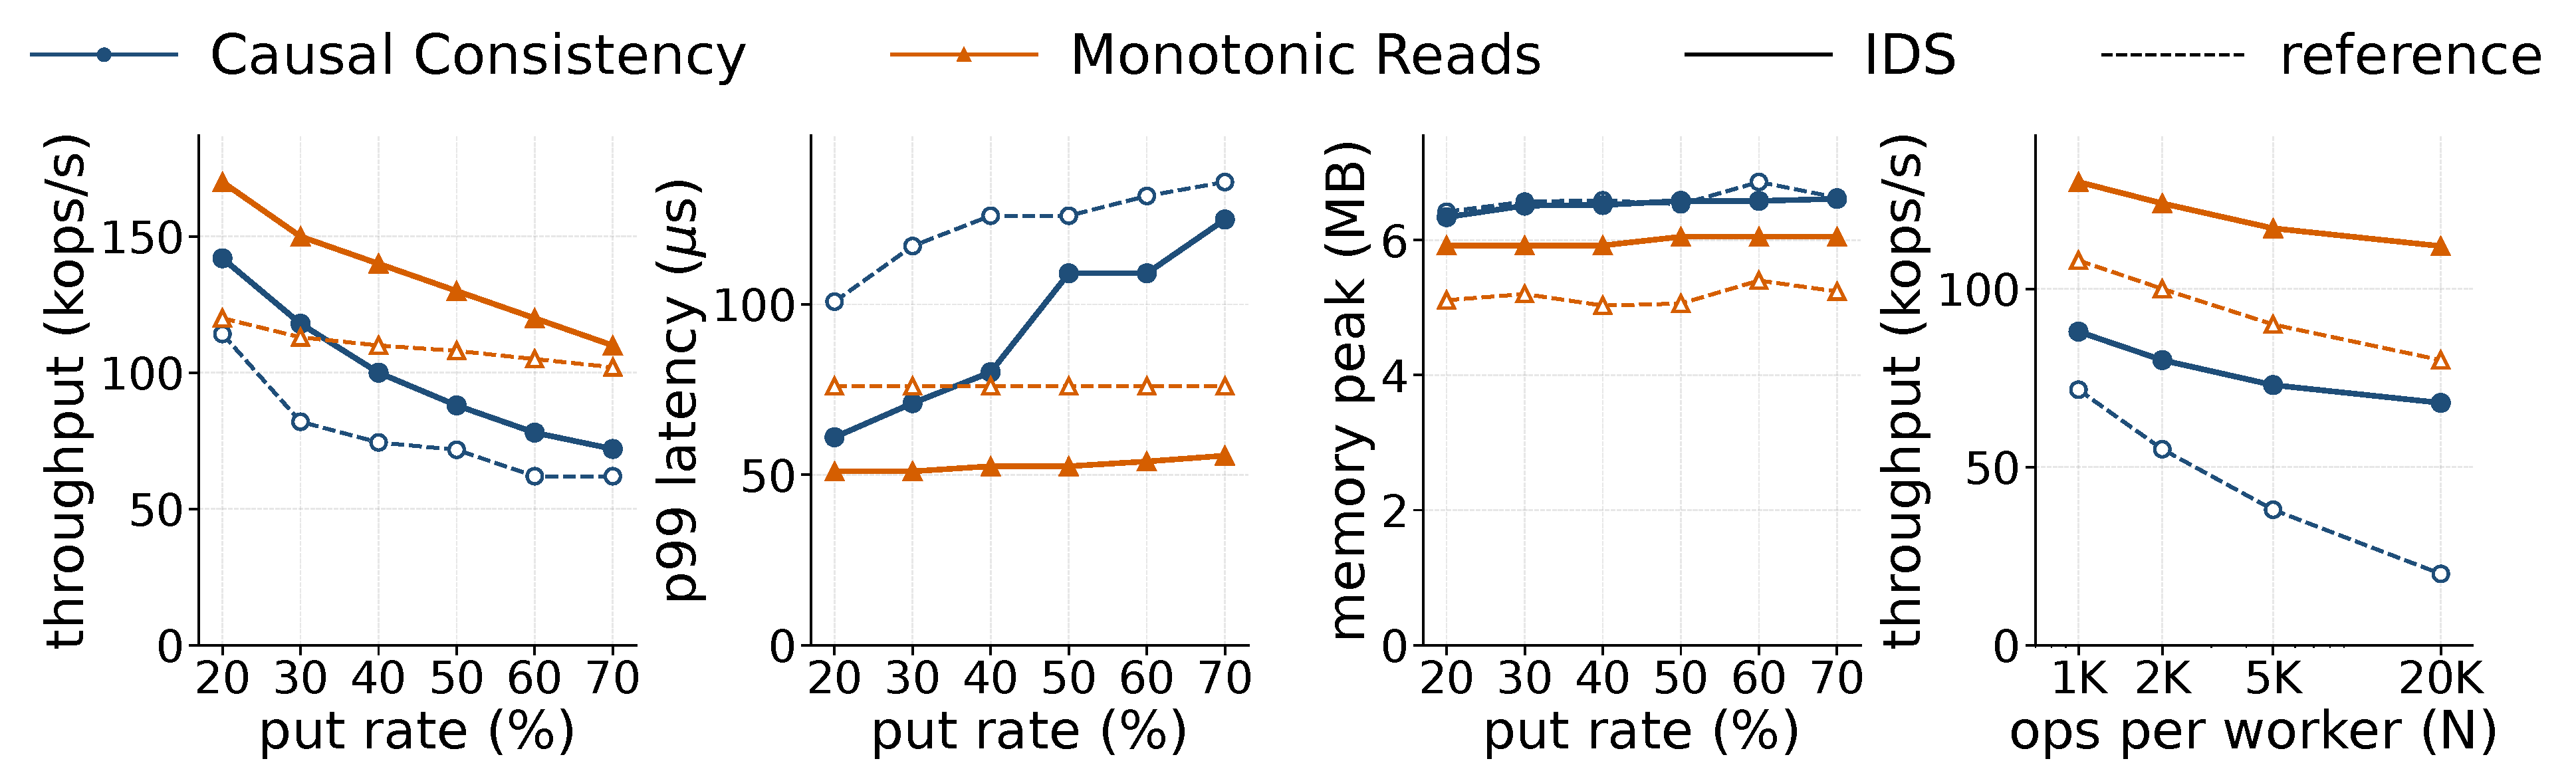
\includegraphics[width=\linewidth]{figures/eval_perf.pdf}
\caption{Throughput, p99 latency, and peak memory vs.\ put rate, and throughput vs.\ ops-per-worker $N$, for \sys{} suite CC and monotonic reads. Solid $=$ \sys{}; dashed $=$ reference (function-as-map for both). The per-spec breakdown for all seven specifications appears in
% \ion{For first and second graphs, the trends suggest that if we increase the put rate, IDS might be worse than the reference...}
% \shubham{So, Ion: as we increase puts to very high our efficiency tricks are no more useful enough and converges to the normal implementation, which btw is also a good implementation. So, maybe we can justify in that way?}
\cref{app:perf-curves}.}
\label{fig:eval-perf}
\end{figure}


\subsection{Runtime performance}
\label{sec:eval-perf}

\sys{}' synthesized implementations match or beat every prior reference: $3\times$ throughput on Chapar's vector-clock reference, $1.4\times$ on \sys{} suite CC and monotonic reads, comparable on read-your-writes (within $20\%$), and $152$k and $139$k ops/s on MW and RYW+MW where the reference times out at every put rate (\cref{app:perf-curves}). We compare on throughput, p99 latency, peak memory, and ops-per-worker scaling. Figure~\ref{fig:eval-perf} shows \sys{} suite CC and monotonic reads vs.\ the references, and 
% function-as-map
the full per-spec breakdown
% , including Chapar's vector-clock reference, 
is in \cref{app:perf-curves}. The gap follows from one mechanism: 
\sys{}' data-store representations are bounded,
% \mohsen{replaced ``bound per-op cost'' with ``are bounded''. Is that correct?} \shubham{Yes, addressed: ``are bounded'' is the cleaner framing at this abstraction level.}
% by the spec,
while the references' grow with workload size. These representations emerged from the joint code+proof loop: the proof obligation drove the agent to them (\cref{sec:eval-synthesis}). The performance feedback from the benchmark harness then steers the agent toward the fastest among multiple verifying candidates (\cref{sec:eval-ablations}).

\textbf{\sys{} suite CC. \ }
Both implementations enforce causality with one timestamp per client; the data store differs. The reference's function-from-key-to-value extracts to OCaml as a chain that grows per put (every get walks it), while \sys{} uses a balanced-tree map where a lookup costs at most the tree depth. \sys{} reaches up to $1.4\times$ peak throughput at low put rate where gets dominate, with p99 latency up to $1.7\times$ lower. 
The gap narrows at high put rate as broadcast becomes the bottleneck; tail latency tracks the same effect, rising with put rate on both implementations as broadcast queue waits grow. Peak memory is comparable at $1$k ops per worker, since the vector-clock state is bounded by client count rather than put rate; larger workloads would push it upward. On ops-per-worker scaling, the reference's throughput collapses by more than half from $1$k to $20$k ops per worker while \sys{} loses only about a quarter.


\textbf{Other \sys{} suite specifications. \ }
%
Unlike CC, these specs only need per-client guarantees, so they do not pay CC's per-write cross-client coordination cost; their tail latency stays flat across put rate (Figure~\ref{fig:eval-perf}, MR). On the other \sys{} suite specs, \sys{} ranges from comparable on read-your-writes (chain stays short) to a gap large enough that the reference times out at every put rate on the monotonic-write specs (MW, RYW+MW). 
The four with prior references (RYW, MW, MR, RYW+MW) share the closure-chain mechanism: the reference's function-from-key-to-value extracts as a chain that grows per put; \sys{} replaces it with a flat list or balanced tree, and the speedup tracks how often the chain is walked. 
% 
On the monotonic reads benchmark, a get in the reference walks every operation, so \sys{} outperforms it by $1.4\times$.

% \mohsen{The plots for the following specs is not shown in the main body. They are too detailed and should be taken to the appendix. Commented below.} \shu{Addressed: the commented detail block is dropped; per-spec plots and the RYW/MW/RYW+MW/LCC/MW-pivot detail are in \cref{app:perf-curves}.}


\subsection{Ablations and Generalization}
\label{sec:eval-ablations}

The joint step-wise discovery of code and proof is the key design decision behind \sys{}.
% The agent baselines in \cref{sec:eval-synthesis} fail because they are not step-wise.
We ablate this joint design itself ($-$J), the ISA's proposer ($-$P) and reloader ($-$R), the coordinator's audit step ($-$A), and the \coq{} feedback to the DSA ($-$VF) across the seven key-value store specs and VERINA's $189$ Lean tasks (Table~\ref{tab:eval-ablation}). We also evaluate the DSA alone and \sys{}' prover component decoupled from the rest of the system on four cross-language proof benchmarks (DafnyBench, miniCodeProps, Verus-Bench, CoqStoq), where it sets a new state-of-the-art on each.
% \accheng{mention the general prover results here} \shubham{Addressed: added preview sentence about DSA-alone cross-language results.} 

% frozen, the proof phase cannot change course.

\textbf{Architecture ablations. \ }
Without joint discovery, only RYW succeeds in a majority of runs: Chapar CC, RYW+MW, \sys{} suite CC, and LCC drop to $0$ out of $3$, and VERINA falls to $85\%$ ($-8\%$ from full \sys{}' $93\%$). This is because a fixed implementation limits the proof phase. On Chapar CC, $-$J commits to the global per-replica state closest to the spec. Full \sys{} reloads to per-key entries when the proof stalls. 
% (\cref{sec:eval-synthesis} trace). 
The audit step catches trivial solutions that pass \coq{}'s type-checker: 
on \sys{} suite CC, an agent without auditing once shipped a \texttt{put-guard} returning \texttt{false} unconditionally, with the theorem being trivially satisfied. On the other hand, cells under $-$A count only audited successful runs. 
% 
Ablations of the proposer and reloader each drop pass rate on the four hardest specs (Chapar CC, MR, \sys{} suite CC, LCC), taking VERINA to $79\%$ ($-14\%$) under $-$P and to $88\%$ ($-5\%$) under $-$R. 
% 
The \coq{} feedback to the DSA is the most consequential single component: 
replacing the structured \coq{} diagnostic (goal, hypotheses, tactic backtrace)
% \mohsen{What is structured diagnostic?} \shubham{addressed: parenthetical (goal, hypotheses, tactic backtrace) inlined.}
with only an accept/reject drops every spec to at most $1$ of $3$ successful runs and VERINA to $58\%$ ($-35\%$). 
% \shu{this reads arelaly dense, and with -J, -P, -R, which are really hard to parse... need to rephrase this to be better}
% \shu{this can be shrinked further to half a page if we are space-constrained}
% \mohsen{This paragraph is long but more readable than the previous long ones in this section.} \shu{Noted; left this paragraph as-is.}

\textbf{Performance-feedback ablation. \ }
Without performance feedback ($-$PF), the agent commits to the first implementation and proof that passes the type-checker and misses the course-corrections seen in \cref{sec:eval-perf}. 
As \cref{fig:eval-bench} shows,
full \sys{} is on average $1.42\times$ faster than $-$PF across the six specs with reference baselines (Chapar CC, RYW, MW, RYW+MW, MR, \sys{} suite CC).
% \accheng{why geomean? can we just say on average?} \shubham{Addressed: changed 'geomean' to 'on average'.}
% \mohsen{Commented the following. Why does it mean? Why do we say it?}
% The performance measurement is a search signal, not a post-hoc metric. 

\textbf{DSA as a general prover. \ }
The DSA's effectiveness is not specific to \sys{}' synthesis loop or to \coq{}: 
applied alone to public verification benchmarks across four languages, it sets a new state-of-the-art on each (Figure~\ref{fig:eval-crosslang}, Table~\ref{tab:bench-results}).
% \shu{as shown in Figure... or Table...} \shubham{Addressed: moved the (Figure, Table) citation up to this sentence.}
% It ties or beats every prior work on four public proof benchmarks across  :
It saturates miniCodeProps ($100$ of $100$) and Verus-Bench ($149$ of $150$), and beats prior SOTA by $36$ to $69\%$ on DafnyBench and CoqStoq. 
% 
% \mohsen{The following line was not clear. Replaced it with the next line.}
% The gain is the architecture, not the model: 
\sys{}' agentic architecture brings further gain:
full \sys{} adds $+10\%$ on DafnyBench, $+20\%$ on miniCodeProps, and $+51\%$ on CoqStoq over Codex under the same prompt, while a baseline-model swap (Codex $\to$ Claude under the same prompt, no \sys{} architecture) gains at most $6\%$ on any of these four benchmarks. 
% 
\sys{} also reaches state-of-the-art on all three code-and-proof benchmarks: $176/189$ on VERINA (prior SOTA $38$), $65/77$ on AlgoVeri ($2\times$ prior SOTA $31$), and a full $62/62$ on CloverBench (Table~\ref{tab:bench-results}; detail in \cref{app:benchmarks}).
% \shu{I don't like x/y this kind of writing, the number is sort of meaningless to me, maybe switch to percentage} \accheng{I would be consistent, we do say like 2 out of 7, 1 out of 3 before so maybe okay to keep. do we show the percentages in table somewhere?} \shubham{Addressed: keeping x/y per Audrey's consistency point. The paper uses x/y throughout (Q1's "2 of 7", §5.2's "3-of-3"/"2-of-3", and tables/bench-results.tex shows "176 / 189" too), so switching just these three prose lines to percentages would diverge from the tables. The "prior SOTA 38" anchor next to 176/189 makes the gap obvious without needing a percentage; "62/62" reads punchier as full saturation than "100\%".}


\begin{figure}[t]
\centering
% \begin{minipage}[b]{0.27\linewidth}
\begin{minipage}[b]{0.3\linewidth}
\centering
\providecolor{rowhl}{HTML}{EFF3F8}
\centering
% \tiny
\scriptsize
\setlength{\tabcolsep}{1.1pt}
\renewcommand{\arraystretch}{1.00}

\begin{tabular}{@{}l cccccc@{}}
\toprule
         & full & $-$J & $-$P & $-$R & $-$A & $-$VF \\
\midrule
\rowcolor{rowhl}
Chapar CC& 3/3 & 0/3 & 0/3 & 0/3 & 1/3 & 0/3 \\
RYW      & 3/3 & 2/3 & 2/3 & 3/3 & 3/3 & 1/3 \\
MW       & 3/3 & 1/3 & 2/3 & 2/3 & 2/3 & 0/3 \\
RYW+MW   & 3/3 & 0/3 & 1/3 & 2/3 & 1/3 & 0/3 \\
MR       & 3/3 & 1/3 & 0/3 & 1/3 & 0/3 & 0/3 \\
\sys{} suite CC& 2/3 & 0/3 & 0/3 & 0/3 & 0/3 & 0/3 \\
LCC      & 3/3 & 0/3 & 0/3 & 0/3 & 0/3 & 0/3 \\
\midrule
\rowcolor{rowhl}
VERINA   & 176 & 160 & 150 & 167 & 176 & 110 \\
\bottomrule
\end{tabular}
\captionof{table}{Component ablations: \# successes from $3$ runs ($189$ tasks for VERINA).}
\label{tab:eval-ablation}

\end{minipage}\hfill
% \begin{minipage}[b]{0.345\linewidth}
\begin{minipage}[b]{0.32\linewidth}
\centering
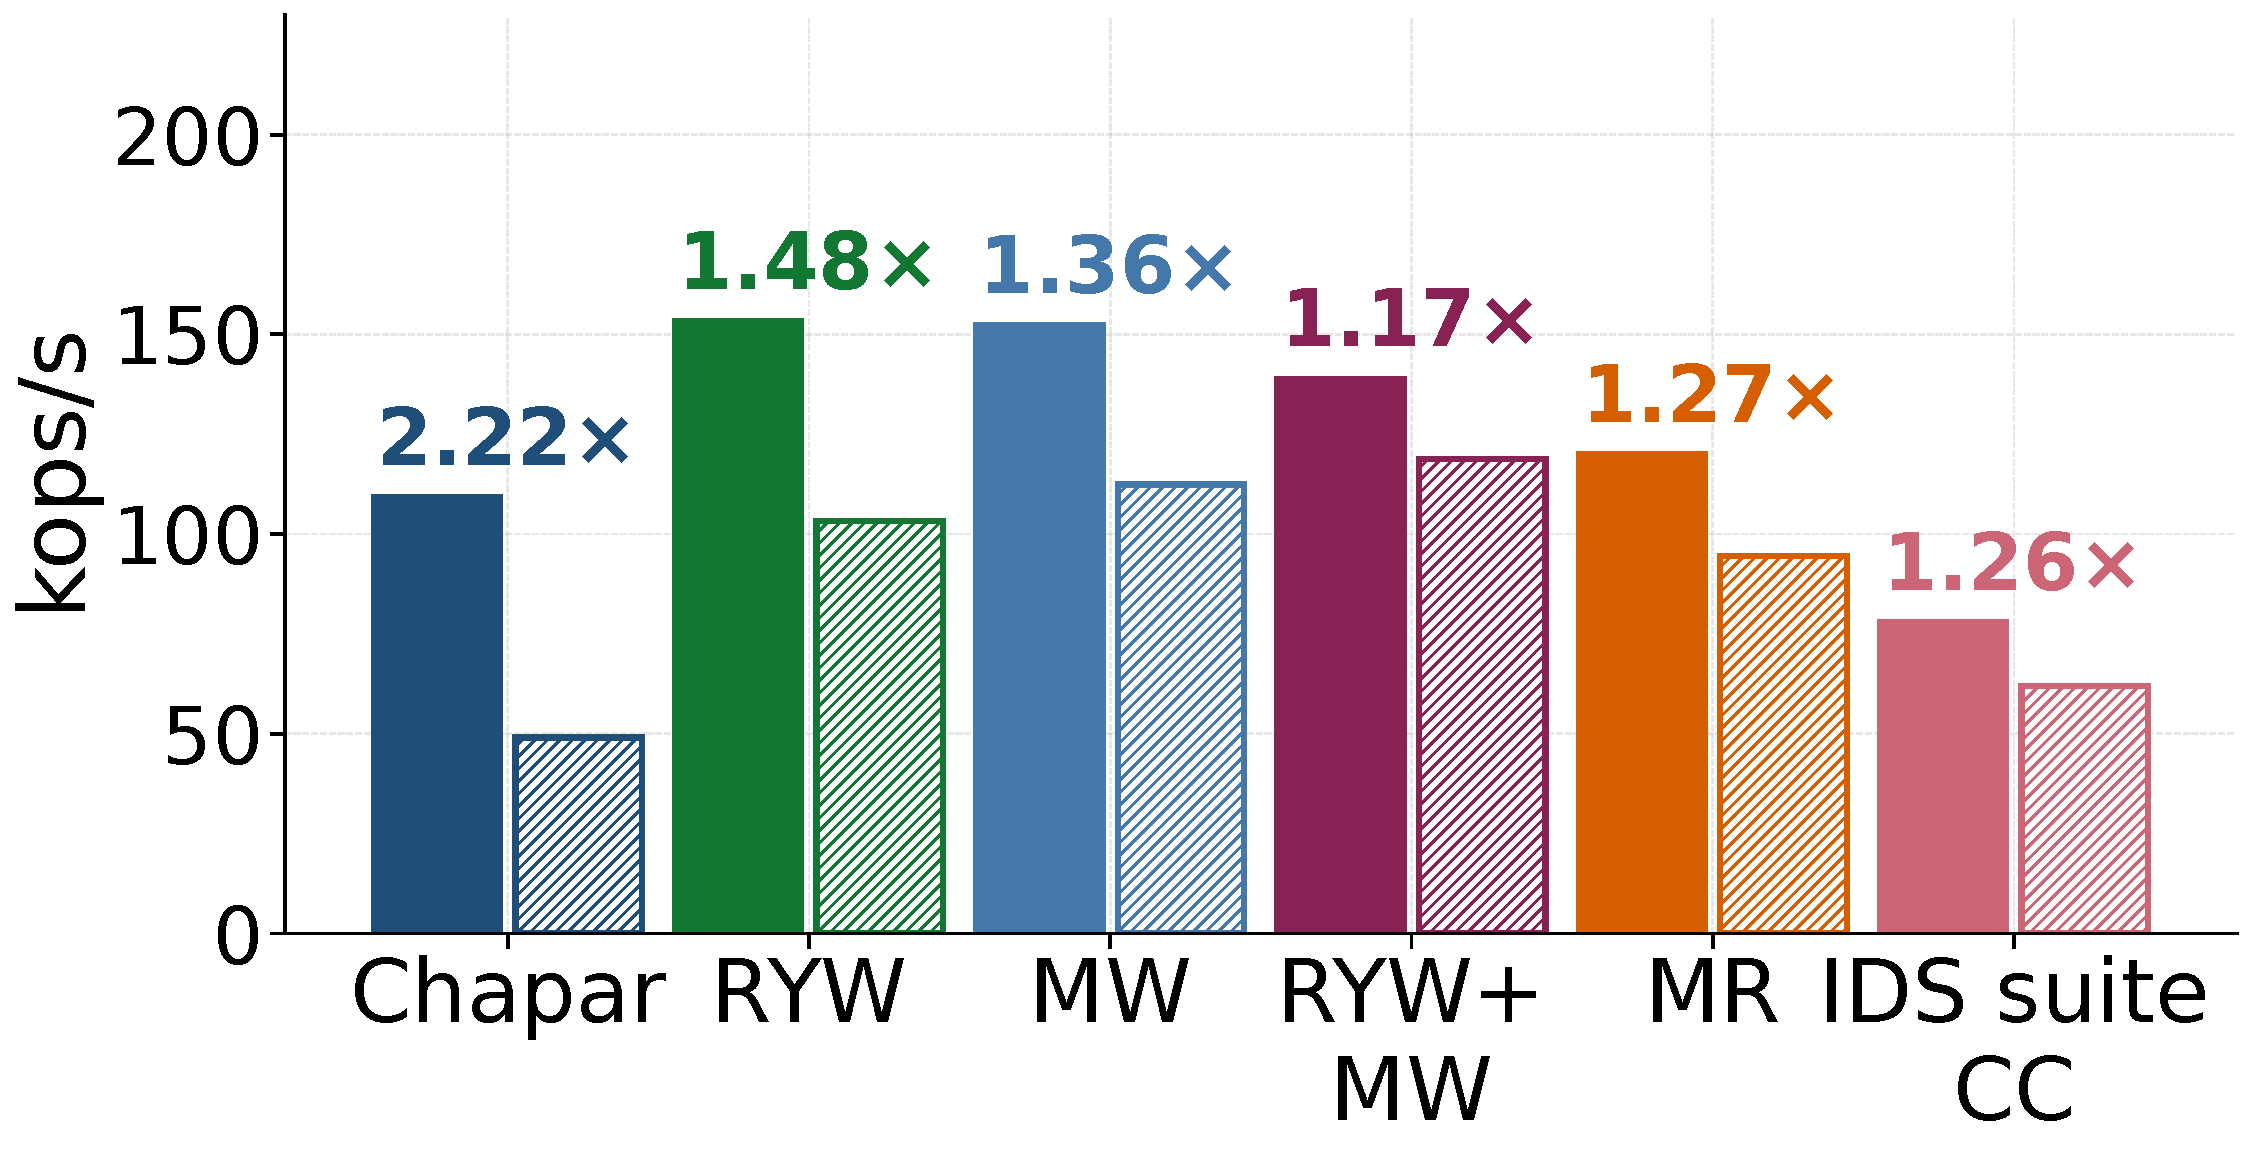
\includegraphics[width=\linewidth]{figures/eval_bench.pdf} \\[1.3em]
\captionof{figure}{Performance-feedback ablation at $\textit{put}=60\%$: \sys{} (solid) vs.\ no-feedback (hatched).}
\label{fig:eval-bench}
\end{minipage}\hfill
% \begin{minipage}[b]{0.345\linewidth}
\begin{minipage}[b]{0.32\linewidth}
\centering
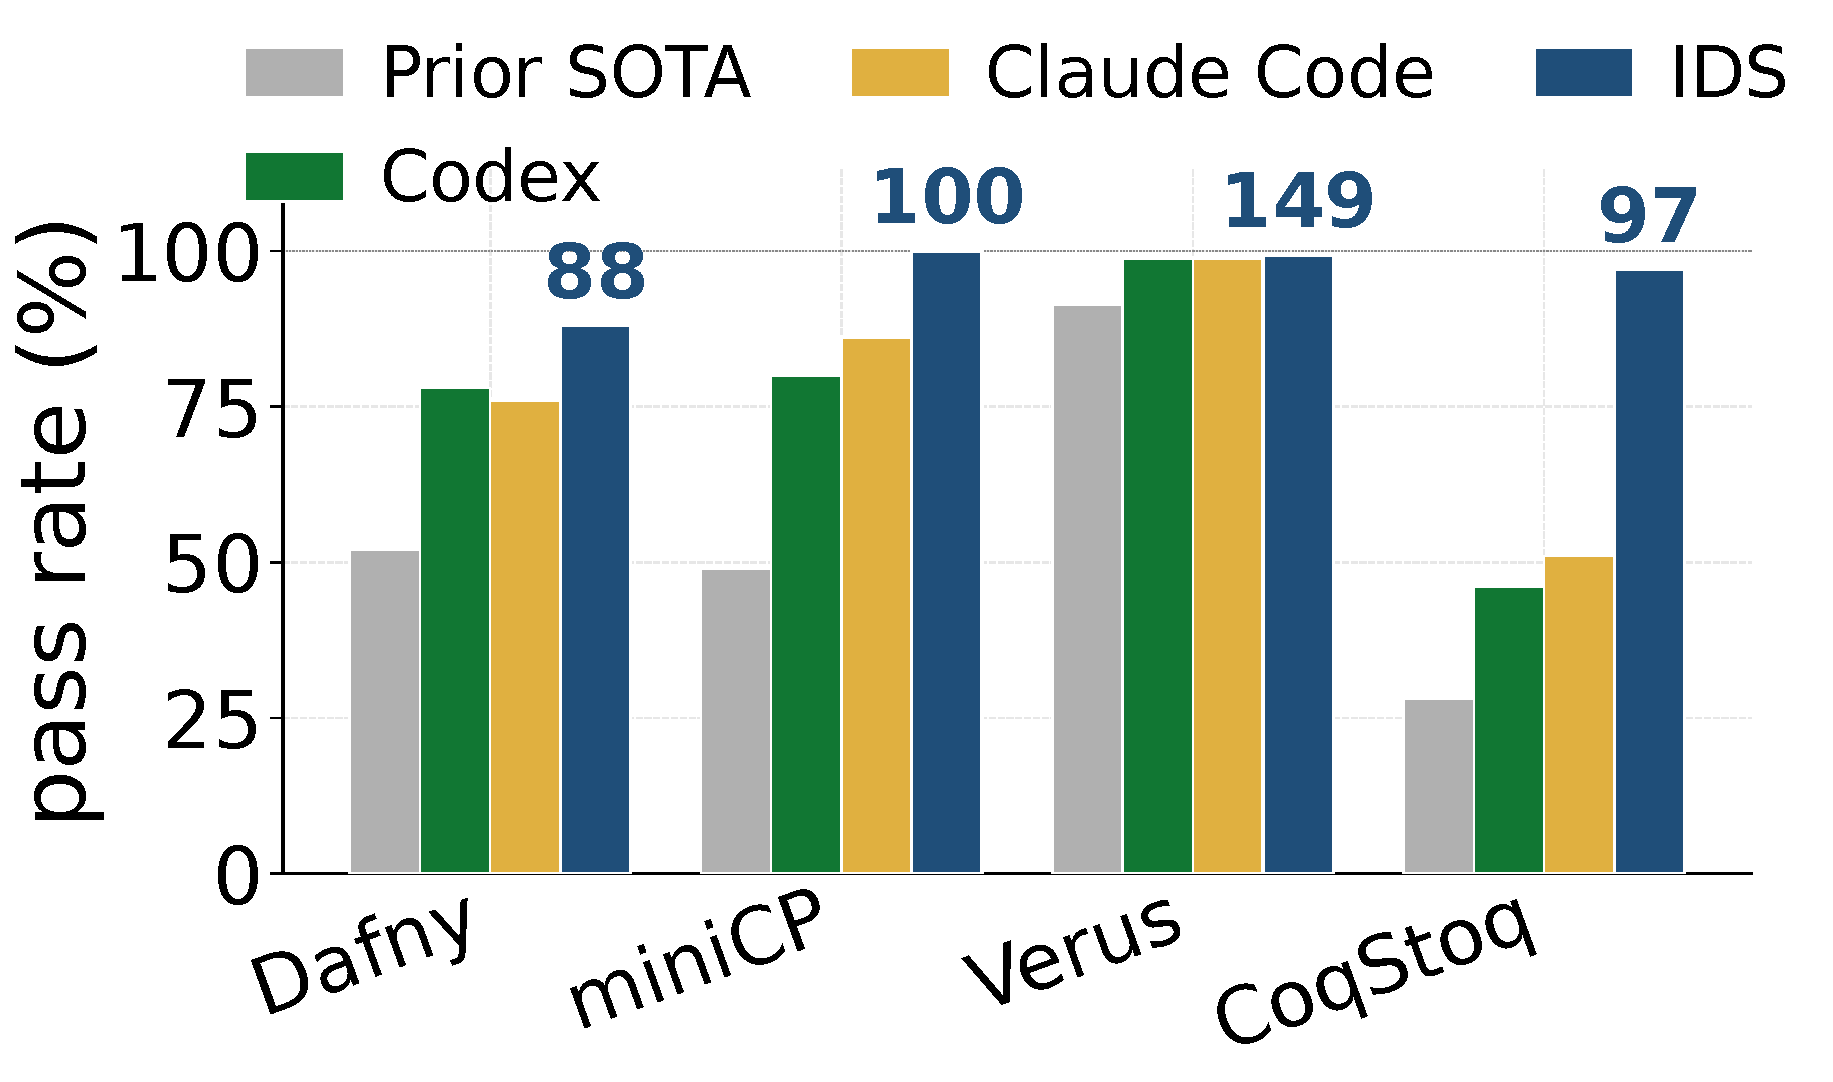
\includegraphics[width=\linewidth]{figures/eval_crosslang.pdf} %\\[0.3em]
\captionof{figure}{Cross-language success rate (\%) on 4 verification benchmarks;
labels are \# of successes.}
\label{fig:eval-crosslang}
\end{minipage}
\end{figure}





\section{Discussion and Conclusion}
\label{sec:conclusion}
\label{sec:discussion}

\aknew{\paragraph{IDS is language- and problem-agnostic.} IDS as a technique depends on neither the verification backend nor the problem domain. The backend need only support (i) mechanical checking of partial proofs, (ii) a programmatic interface an LLM agent can drive, and (iii) executable extraction of verified implementations for performance feedback; Lean~\cite{lean} and Verus~\cite{verus} both qualify, and we expect IDS to transfer to either without structural changes. The problem domain need only admit a machine-checkable formal specification and a way to benchmark candidate implementations. We chose \coq{} for the maturity of its ecosystem, and we chose distributed key-value stores because the literature already provided a complete formal specification for one consistency model; following its structure, we contribute six additional specifications covering other consistency properties (\cref{app:suite}).}

\aknew{\paragraph{Limitations. \ } Our work has three main limitations. First, \sys{} requires a formal \coq{} specification as input; writing complete formal specifications for distributed systems requires substantial expert effort, a challenge we return to below. Second, the seven specifications we evaluate cover correctness-critical behavior but not the full operational envelope of a production KV store; they do not define interfaces for scaling out (adding or removing nodes at runtime), reconfiguration, fault recovery, or informal but practically necessary behavior such as logging and observability endpoints. Given a richer specification that captures these aspects, we see no reason IDS would not apply unchanged, but evaluating this is left to future work. Third, our empirical evaluation covers the distributed key-value store problem only, leaving validation on other domains (e.g., OS protocols, cryptographic primitives) to future work. \cref{app:limitations-impacts} discusses additional limitations and broader impacts.}

\aknew{\paragraph{The specification bottleneck.} While \sys{} automates the synthesis of verified implementations, writing the formal specification itself remains the largest open problem: accurately capturing a system's intended behavior in a machine-checkable form is hard, and any correctness guarantee is only as strong as the specification it is checked against. We envision two directions for closing this gap. First, \emph{adversarial specification synthesis}, in which an LLM agent collaborates with a human stakeholder in natural language, iteratively probing intent and surfacing ambiguities until a formal specification emerges. Second, \emph{specification extraction from existing systems}, in which an agent recovers the correctness properties of a deployed implementation while leaving the design space open, so that \sys{} can synthesize alternative implementations that satisfy the same properties with better performance. We are actively pursuing both directions, which we plan to report on in future work.}

%Verified systems construction has long taken months to person-years of expert effort. \sys{} replaces that effort with compute, in hours: a proving-based regime where an LLM coding agent receives fast, exact correctness feedback with no false positives, turning joint code-and-proof construction into a search problem the agent can drive.

\paragraph{Conclusion. \ } Verified systems construction has traditionally required months to years of expert effort. \sys{} condenses this timeline to mere hours by replacing human labor with compute. By providing an LLM coding agent with fast and exact correctness feedback without false positives, \sys{} transforms the joint code-and-proof construction into an automated search problem. This shifts vibe coding to verified coding by using LLMs to directly build type-safe systems that are machine-checked against a formal specification, effectively eliminating silent bugs and unverified assumptions. Crucially, this methodology generalizes to any domain with a machine-checkable correctness oracle, including OS kernels, compilers, cryptographic protocols, and hardware. Ultimately, \sys{} shows that verified software generation is transitioning from a human-labor bottleneck to a compute-driven approach, paving the way for the broad adoption of verified system synthesis.

\section*{Acknowledgments}
This research is supported by NSF (IFML) CCF-2019844 and gifts from Accenture, AMD, Anyscale, Broadcom Inc., Google, IBM, Intel, Intesa Sanpaolo, Lambda, Mibura Inc., Samsung SDS, and SAP. We also thank our Sky Lab and NetSys colleagues at UC Berkeley for fruitful discussions that shaped this paper.

% proof-driven 
%Future extensions could also try to solve the spec-writing problem with agents and explore joint optimization across other resource axes (memory, energy, latency). Verified software is becoming a compute problem rather than a person-year problem, and adoption will only grow as LLMs are used for certified system building and proof-driven coding beyond what informal review can cover.
% Verified systems construction has long taken months to years of expert effort. IDS replaces that effort with compute in hours: by synthesizing both the implementation and its proof incrementally and in lockstep, IDS turns formal verification into a search problem. The agent receives fast feedback from a formal checker to rule out dead ends, while a distributed testbed evaluates throughput to steer the search toward efficient implementations. This enables agents to autonomously generate complex distributed systems with end-to-end formal correctness guarantees, avoiding the silent bugs that escape standard testing. The specification itself still has to be written by a person, but everything that follows can be discovered, and the recipe could apply wherever a machine-checkable correctness oracle exists (OS kernels, compilers, cryptographic protocols, hardware). Future extensions could try to solve the spec-writing problem with agents and explore joint optimization across other resource axes (memory, energy, latency). Verified software is becoming a compute problem rather than a manual problem, and adoption will only grow as LLMs are used for certified system building beyond what informal review can cover.

{\small
\bibliographystyle{plain}
\bibliography{references,refs}
}

\clearpage
\appendix
% Type all labels defined in the appendix as `appendix' so cref renders
% them via the App.~ format declared in the preamble. Cleveref also
% auto-derives `subappendix' and `subsubappendix' from sectioning depth.
\crefalias{section}{appendix}
\section{Specifications and the \sys{} Suite Dataset}
\label{app:consistency-specs}

Of the seven specifications evaluated in \cref{sec:eval}, one is Chapar's published causal-consistency spec~\cite{chapar} and the other six are \sys{} suite specs we wrote with a formal-verification and distributed-systems expert ($1{,}018$ lines of \coq{} across five spec files; RYW+MW is the joint composition of RYW and MW with no separate spec; \cref{tab:eval-specs-summary}). Formal definitions are in \cref{app:suite}, which also gives two reference implementations of \sys{} suite CC (vector-clock and dependency-map variants) and the Lloyd-Freedman protocol (the COPS causal-consistency protocol) as a systems-scale reference.

\begin{table}[h]
\centering
\footnotesize
\setlength{\tabcolsep}{6pt}
\renewcommand{\arraystretch}{1.05}
\caption{The seven specifications. Chapar CC is a published spec; the six \sys{} suite specs are expert-written for this paper. \emph{Property} summarises the consistency guarantee; \emph{LoC} is lines of \coq{} for the spec definition.}
\label{tab:eval-specs-summary}
\begin{tabular}{@{}l l p{0.50\linewidth} r@{}}
\toprule
Specification    & Family       & Property                                                                              & LoC \\
\midrule
Chapar CC        & Chapar       & cross-client causal consistency, defined over execution traces                        & n/a \\
\midrule
Read-Your-Writes & \sys{} suite & a client reads its own most recent write                                              & $159$ \\
Monotonic Writes & \sys{} suite & a client's writes are observed in order                                               & $158$ \\
Monotonic Reads  & \sys{} suite & a client's reads respect the order of observed writes                                 & $185$ \\
RYW+MW           & \sys{} suite & composition of RYW and MW (no separate spec)                                          & n/a \\
CC  & \sys{} suite & cross-client causal consistency via explicit dependency sets                          & $248$ \\
LCC              & \sys{} suite & causal consistency parameterised by per-message labels and per-client interest masks  & $268$ \\
\bottomrule
\end{tabular}
\end{table}

\paragraph{Common shape.}
Every spec is a \coq{} \texttt{Module Type} with the same seven method signatures (\texttt{getReq}, \texttt{getGuard}, \texttt{get}, \texttt{getRes}, \texttt{putReq}, \texttt{putGuard}, \texttt{put}), a \texttt{State} type, an \texttt{Update} type, and an operational semantics on client-replica configurations. \sys{} consumes this shape directly.

\paragraph{Generality.}
\sys{} is not tuned to any individual spec: the same agent, prompts, and tools handle every spec we evaluate. Any specification matching the \texttt{Module Type} shape above is a candidate target for the same loop.
   % A. Specifications and \syst{} suite
\section{Synthesis Results: Per-Spec Artifacts}
\label{app:synth-results}

All seven artifacts pass \coq{}'s kernel with no \texttt{Admitted}, \texttt{Axiom}, \texttt{Hypothesis}, or \texttt{Parameter}. The three CC specs (Chapar CC: $3{,}037$ lines / $79$ lemmas; \sys{} suite CC: $3{,}807$ / $121$; LCC: $3{,}924$ / $128$) are $4$--$6\times$ larger than the four session specs because their proofs span all replicas, not just sender and receiver.

\begin{table}[h]
\centering
\footnotesize
\setlength{\tabcolsep}{6pt}
\renewcommand{\arraystretch}{1.05}
\caption{Per-spec implementation choice and proof artifact size. Lemmas $=$ \texttt{Qed} count; lines via \texttt{wc -l}.}
\label{tab:synth-artifacts}
\begin{tabular}{l l r r}
\toprule
Specification & Implementation & Lines & Lemmas \\
\midrule
Chapar CC & per-key store entry with sender clock + dep vector & 3{,}037 & 79 \\
RYW       & per-key (val, client, ts) assoc-list & 622 & 25 \\
MW        & per-key (val, client$\to$ts) assoc-list & 722 & 30 \\
MR        & per-(key, client) assoc-list, replace-on-write & 1{,}063 & 30 \\
RYW+MW    & per-key (val, client, client$\to$ts) assoc-list & 958 & 28 \\
\sys{} suite CC & vector clock + per-key VC map + balanced-tree store & 3{,}807 & 121 \\
LCC       & vector clock + per-key VC map + balanced-tree store + per-client label-set filter & 3{,}924 & 128 \\
\bottomrule
\end{tabular}
\end{table}


\paragraph{Implementation rationale.}

\textbf{Chapar CC.} The $79$ lemmas split: $11$ per-method refinement (one per \texttt{get}/\texttt{put}/\texttt{update}/\texttt{guard}/\texttt{init}), $11$ reachable-state invariants, $7$ causality preservation, $39$ clock and per-key store algebra, and $11$ execution-model helpers.

\textbf{Session guarantees (RYW, MW, MR, RYW+MW).} All four share the same assoc-list skeleton; each parameterizes the per-entry payload to its consistency property: RYW carries (val, client, ts) to detect own writes, MW extends to (val, client$\to$ts) to enforce writer order, MR uses one entry per (key, client) updated in place, RYW+MW combines both. The proof technique is shared too: each session uses heavy case-analysis via \texttt{Nat.eq\_dec} on key and client equality ($80$--$100$ splits per spec), varying only in which payload field the splits land on. Each Get scans only the distinct keys touched, not the full Put history. MR is the hardest session spec because its Put proof splits into four sub-cases (same vs different key, same vs different client), each closed by case-analysis on \texttt{Nat.eq\_dec}.

\textbf{\sys{} suite CC.} A vector clock, a per-key vector-clock map, and a balanced-tree store; the balanced tree keeps Get logarithmic in distinct keys rather than linear in prior Puts. Of the $121$ lemmas: $8$ are the step-by-step simulation, $32$ are refinement-relation invariants for the state components (cell, replica, snapshot) and their preservation under updates, $19$ are vector-clock algebra; the remaining $62$ are update, lookup, owner, and dependency-tracking algebra. Get's proof closes by applying the relation that ties the implementation's vector clocks plus per-client owner lists (per-key tracking of which client most recently wrote each entry) to the spec's dependency sets.

\textbf{LCC.} A vector clock, a per-key vector-clock map, and a balanced-tree store, with dependency entries tagged with a label (a $4$-tuple of client, timestamp, key, label) and projections at Get filtered by the requesting client's interest mask. The proof closes by step-by-step simulation; the simulation relation ties the implementation's label-tagged vector-clock representation to the spec's label-filtered dependency sets. Of the $128$ lemmas: $6$ are the step-by-step simulation, $25$ are refinement-relation invariants and extensions for state components (cells, replicas, snapshots, key-snapshots), $19$ are vector-clock algebra; the remaining $78$ are update, lookup, owner, and dependency-tracking algebra.

\paragraph{Synthesis trajectories.}
The artifacts above are not the first design \sys{} attempted. In each case, the proof stalled on a goal that resisted splitting under the spec's natural state representation; the ISA's reloader abandoned the branch, and the proposer pivoted to a representation under which the goal decomposed.

\textbf{Chapar CC.} The hardest case in any causal-consistency proof shows that whenever a replica delivers a remote message, it has already observed every update the message transitively depends on. \sys{}' first attempt kept the global state representation closest to the spec, under which the delivery lemma had to range over every in-flight message at every replica together, and the DSA could not split it. After the search stalled, the reloader abandoned that branch and the proposer revised the design to a per-key store with per-entry sender, sender-clock, and dependency vector. The proposer then split the delivery invariant into three sub-lemma classes (per-message, per-store-entry, per-replica-clock), each closing under the new representation. The representation was chosen by what split the proof, not by performance; the per-put performance win reported in \cref{sec:eval-perf} is a consequence.

\textbf{Monotonic reads.} Both agent baselines, and \sys{}' first attempt, stalled on the function-from-key-to-value representation. After the reloader abandoned that branch, the agent revised the design to a flat list of per-(key, client) entries updated in place, after which the put proof split into four sub-cases on key and client equality.

\textbf{\sys{} suite CC and LCC.} The winning move is to break the simulation goal into per-message and per-store-entry sub-lemmas, each closing against the per-key store and label-tagged dependency entries respectively. The baselines try the combined goal in one shot and time out within the budget.
 % D. Synthesis results detail
\section{Implementing Distributed-KV Specifications with Coding Agents \\(No Proof)}
\label{app:llm-only-synthesis}

\paragraph{Setup.}
We test Codex (\texttt{gpt-5.4}) on four KV-store consistency properties (RYW, MW, MR, and CC). For each property, Codex generates 100 candidate implementations under two prompt conditions, then picks its single best candidate. That selected implementation is the agent's output for that (property, condition).

\emph{Setting (1) Spec-Given.} Codex receives the formal \coq{} specification and the module-type signature.

\emph{Setting (2) NL-Only (``vibe coding'').} Codex receives only a one-paragraph natural-language description of the property (reproduced verbatim below) and the module-type signature.

Each of the 100 generation sessions runs independently and can compile, edit, and test its own code. The selector pass is also Codex, with the same compile and test access. The selected implementation must use bounded state, cannot copy any reference implementation, and cannot use \texttt{Admitted}, \texttt{Axiom}, \texttt{Hypothesis}, or \texttt{Parameter} (so the agent cannot stub out unfilled work). The agent does not write any refinement proof.

We evaluate the selected implementation in two stages.
\emph{Stage~1 (test).} We run the implementation on an adversarial multi-client scenario; if it accepts an operation the abstract specification rejects on this scenario, Stage~1 fails.
\emph{Stage~2 (proof).} If Stage~1 passes, \sys{} attempts the refinement proof against the abstract specification. If \sys{} cannot close the proof within budget, Stage~2 fails.
We split into two stages because proof attempts are much more expensive than scenario testing. If Stage~1 fails, Stage~2 fails too: an implementation that breaks the spec on a single trace cannot be proven correct on every trace.

\paragraph{Property statements (LLM-visible in Setting~2).}
\begin{description}
\item[RYW (Read-Your-Writes).] Each client must observe its own previous writes. If a client writes a value to a key and later reads that key in the same session, the read must return the client's value or a more recent one.
\item[MW (Monotonic Writes).] Writes by the same client are applied at every replica in the order the client issued them.
\item[MR (Monotonic Reads).] Successive reads by the same client observe non-decreasing replica states: once a client has seen a value, later reads must not appear older.
\item[CC (Causal Consistency).] If operation $A$ causally precedes operation $B$ (either $A$ comes before $B$ in the same client's session, or $B$ reads a value written by $A$), every client that sees $B$ must also have seen $A$.
\end{description}

\begin{table}[h]
\centering
\small
\begin{tabular}{l|ccc|ccc}
\toprule
 & \multicolumn{3}{c|}{Setting (1) Spec-Given} & \multicolumn{3}{c}{Setting (2) NL-Only} \\
Spec & Stage~1 pass & Stage~2 pass & Cost & Stage~1 pass & Stage~2 pass & Cost \\
\midrule
RYW & 1 & 1 & \$30.50 & 1 & 0 & \$25.77 \\
MW  & 1 & 0 & \$32.10 & 1 & 0 & \$27.33 \\
MR  & 0 & 0 & \$35.20 & 0 & 0 & \$29.91 \\
CC  & 0 & 0 & \$47.80 & 0 & 0 & \$40.79 \\
\bottomrule
\end{tabular}
\caption{Outcome of best-of-$N{=}100$ implementation-only synthesis with Codex. \textbf{1} = passed, \textbf{0} = failed. Stage~1: the selected implementation runs through a fixed adversarial multi-client scenario without violating the abstract specification on that scenario. Stage~2: \sys{} builds a refinement proof of the implementation against the abstract specification within budget. Cost is the \texttt{gpt-5.4} token cost for the 100 generations plus the selection pass.}
\label{tab:llm-only-synthesis}
\end{table}

\paragraph{Result and takeaway.}
Best-of-$N=100$ produces a verified implementation on 1 of 4 properties when given the formal specification (Setting~1, RYW), and on 0 of 4 from natural language alone (Setting~2). The two simpler session properties (RYW and MW) consistently pass the scenario test in both settings, but only RYW with the formal spec also passes the refinement proof. The harder properties (MR and CC) fail even the scenario test in both settings: the textbook patterns Codex selects (vector-clock dominance, last-write-wins) do not implement the per-key or causal-order behavior these specs demand. Two failure modes appear: (a) implementations that fail on a single adversarial trace, and (b) implementations that pass the trace but cannot be proven correct on every reachable state. \sys{} avoids both by integrating the refinement proof into synthesis rather than running it as a post-hoc check; in the main evaluation it closes the proof on all 7 specifications.
 % D2. LLM-only synthesis (pass@K=100 NL)
\section{Additional Performance Results and Throughput Breakdown}
\label{app:perf}
\label{app:perf-harness}

\sys{}' gains over the reference implementations all share one mechanism: \sys{}' state representations bound per-op cost by the spec, while the references' per-op cost grows with workload size. \cref{app:perf-curves} measures this on all five \sys{} suite specs with cluster-runnable implementations (RYW, MR, MW, RYW+MW, \sys{} suite CC), shows Chapar CC at the top of the figure for comparison, and adds an illustrative LCC row (labeled causal consistency: each client subscribes to a set of topic labels and only sees causality enforced on those). Across the \sys{} suite, throughput tracks consistency strength (RYW $>$ MW $>$ RYW+MW $>$ MR $>$ LCC $>$ \sys{} suite CC at put $=50\%$) because stricter specs require more checking work per operation. Chapar CC and \sys{} suite CC are both causal-consistency variants but their reference implementations are designed differently (Chapar's reads one position out of a flat list of per-write dependencies, while \sys{} suite's compares an entire per-client clock vector and atomically updates the writer's slot on every Put), so the two CC rows show different per-op work at the same correctness level. \cref{app:perf-cc,app:perf-mr} decompose the gap on Chapar CC and Monotonic Reads.

\paragraph{Setup details (extending \cref{sec:eval-setup}).}
Cluster zone: \texttt{us-central1-f}. Each VM is an \texttt{e2-standard-2} (2 vCPU, 8\,GB RAM) on Debian 12. Toolchain: OCaml 4.13.1 (dune 3.10) and \coq 8.18.0. Throughput is the sum across the $\text{NW}=4$ workers of $N / t_w$, where $t_w$ is each worker's wall-clock time and $N$ is its ops count, taking the median over three runs per cell; the put-rate sweep uses $N=1000$ (4{,}000 cluster ops total per run) and the scaling sweep varies $N \in \{1{,}000, 2{,}000, 5{,}000, 20{,}000\}$. Per-operation latency is bracketed inside the runtime around \texttt{put\_method}/\texttt{get\_method} and merged across workers; p99 is the 99th percentile of the pooled per-op latency distribution. Peak memory is the worker maximum of \texttt{Maximum resident set size} from \texttt{/usr/bin/time -v}, taking the median over three runs. Workload parameters: $\texttt{key\_range}=50$, $\texttt{val\_range}=100{,}000$, fixed seed $42$. The cluster uses a Chapar-style UDP runtime (\texttt{runtime\_doctex.ml}) adapted to the seven-method doctex \texttt{AlgDef} interface; we patched a socket bug for OCaml 4.13 / Debian 12.

\subsection{Per-protocol curves: all five \sys{} suite specs}
\label{app:perf-curves}


\paragraph{Result.}
Read-then-write specs cause the reference to exceed our $180$\,s wall-clock cap at every put rate measured: in \cref{fig:eval-perf-appendix} the reference's MW and RYW+MW rows show red $\times$ at every cell, with no measurable throughput. \sys{} runs cleanly throughout: $152$ kops/s on MW and $139$ kops/s on RYW+MW at put $=60\%$. The mechanism is a closure chain: the reference stores per-replica state as a function from key to value (a function-as-map); after extraction to OCaml, each prior \texttt{Put} adds a nested closure that a \texttt{Get} must unwrap. The read-then-write check re-evaluates this chain on every \texttt{Put}; combined with UDP packet reordering and the protocol's no-retry compare-and-swap, throughput collapses to zero. RYW has no read-then-write check, so its reference is competitive with \sys{} across the put-rate sweep: within roughly $20\%$ in either direction depending on workload mix, with \sys{} winning at low put rate (pct$=20$) and the reference faster at high put rate (pct$=60$--$70$). The reversal is a per-Put cost trade: \sys{}' assoc-list rewrites its spine on every \texttt{Put} ($O(K)$ cell allocations, $K$ = unique keys touched), while the reference's function-as-map prepends a single closure layer per \texttt{Put} ($O(1)$ heap cell). At low put rate the assoc-list's $O(K)$ \texttt{Get} lookup beats the reference's closure-chain walk; at high put rate the per-\texttt{Put} allocation cost dominates. MR shows the same chain-walk cost on \texttt{Get} (per-layer slope quantified in \cref{app:perf-mr}); \sys{} suite CC follows the same mechanism with \sys{}' balanced-tree store keeping Get logarithmic in distinct keys. Memory: \sys{}' assoc-list pays $0.1$--$1.0$ MB more on RYW (per-entry overhead) and runs in the same $5$--$6$ MB envelope as the reference on the other specs where the reference completes; on MW and RYW+MW the reference produces no memory measurement (it never completes a run). All memory traces are at $N=1{,}000$ ops/worker; \sys{} suite CC's vector-clock state is $O(\text{\#clients})$, so its trace is flat across the put-rate sweep at this workload size. At substantially larger $N$ or more clients, the message-bus and per-cell deps would push memory upward. The rightmost column (throughput vs $N$ at put $=50\%$) confirms the mechanism on every spec: the reference's throughput drops as $N$ grows because each new \texttt{Put} extends the chain, while \sys{}' assoc-list and balanced-tree structures keep throughput approximately flat. Across the put-rate sweep, both implementations' throughput falls and p99 latency rises as put-rate increases because each \texttt{Put} is broadcast to every replica, so more writes mean more in-flight messages and longer per-op queue waits.

\paragraph{Course correction on MW.}
Without performance feedback, \sys{} ships the first verifying design: a balanced-tree store. With performance feedback, the agent runs both candidates in its microbench harness and converges on the assoc-list, which the cluster benchmark harness confirms at $152$k ops/s at put $=60\%$ (\cref{fig:eval-perf-appendix}). Performance feedback changes the search policy, not the correctness criterion; both candidates are verified \sys{} suite refinements.

\subsection{Throughput breakdown: Chapar CC}
\label{app:perf-cc}

\begin{figure*}[t]
\centering
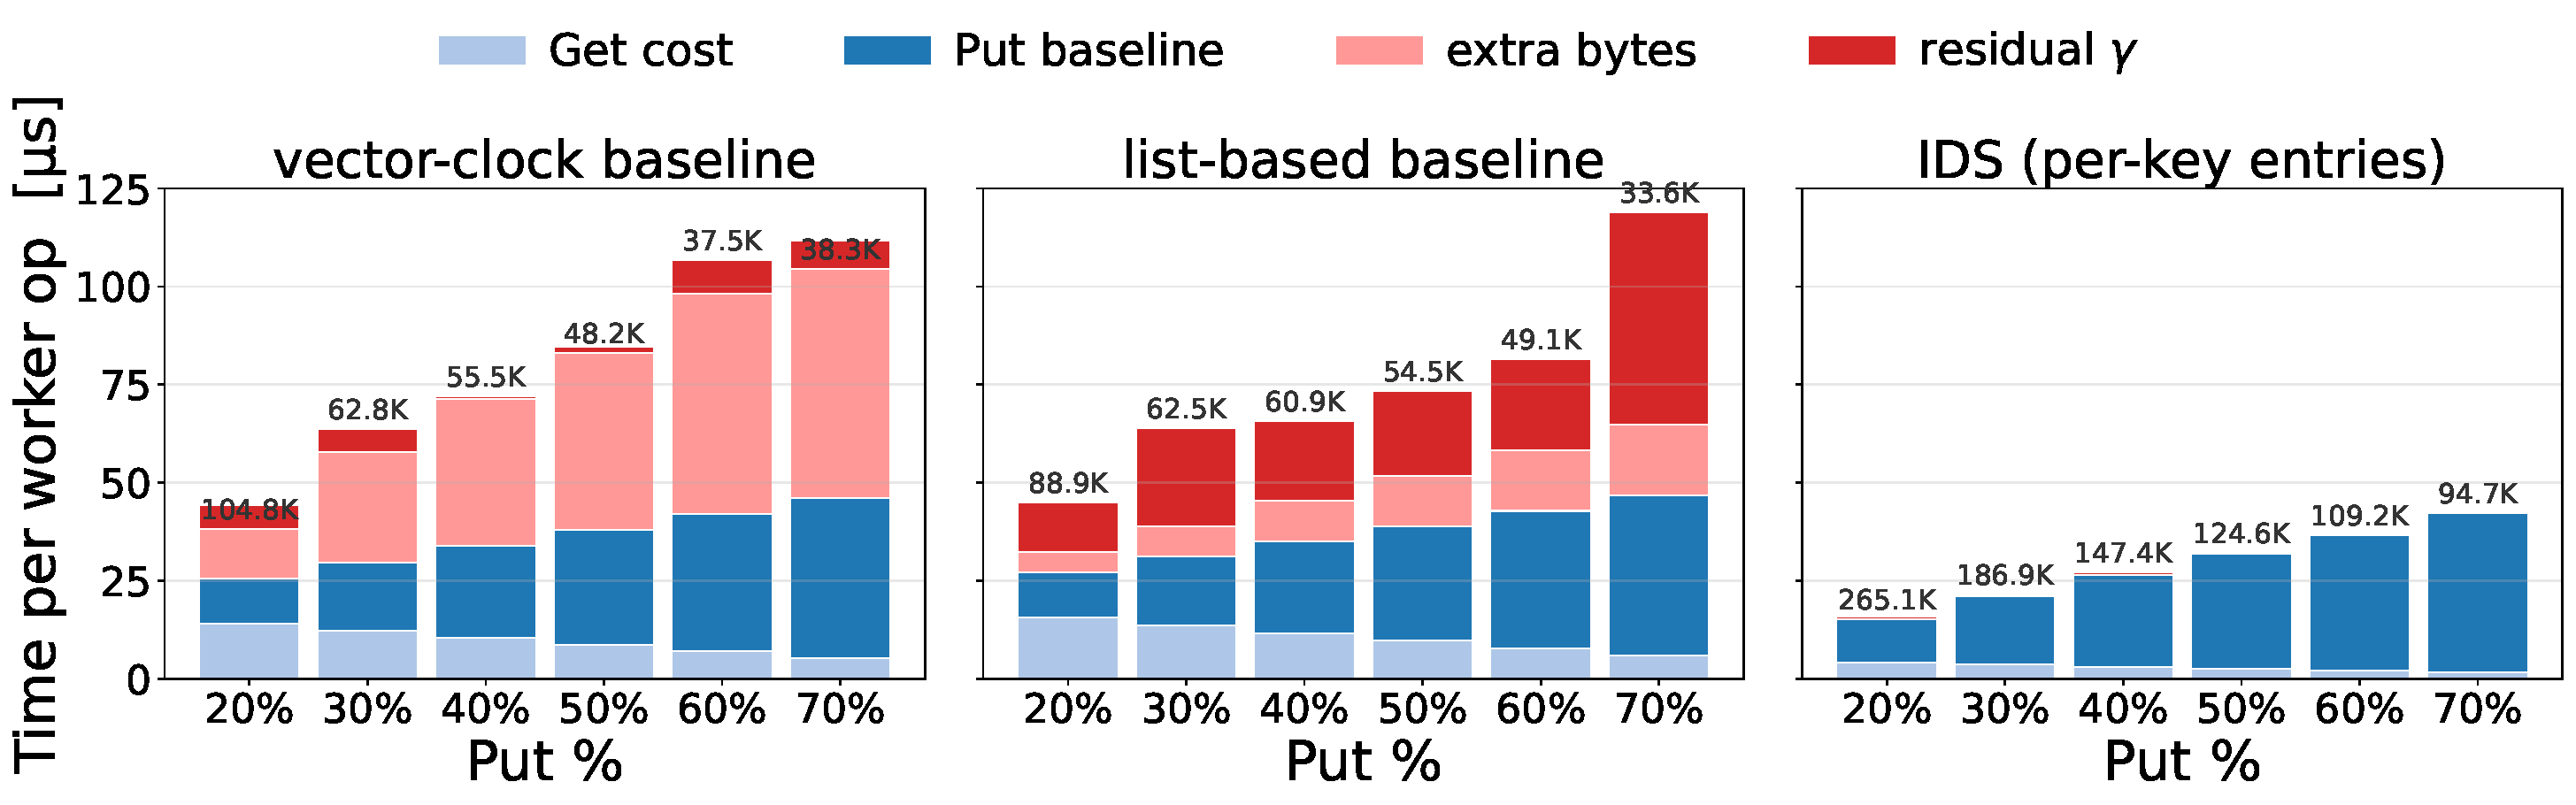
\includegraphics[width=\linewidth]{figures/figure_chapar_decomp.pdf}
\caption{Per-component decomposition of Chapar's two published baselines (vector-clock, list-based) and \sys{}' Chapar implementation (per-key store entries, used here as internal pivot). Bar height equals $4 / \text{(published cluster throughput)}$ in $\mu$s per worker op. Each bar splits into local Get cost, the per-key-entries Put baseline (same for all), per-algorithm extra wire bytes, and a per-algorithm residual $\gamma$. Segments sum to the published value at every cell by construction.}
\label{fig:chapar-decomp}
\end{figure*}

\paragraph{Setup.}
We attribute each algorithm's per-op time to four pieces: its Get cost (varies by algorithm), a shared Put baseline (per-key entries: $58.4\,\mu$s, the smallest of the three), a wire-bytes term proportional to extra bytes per Put ($\beta = 18\,\mu$s per byte, fit from vector-clock vs per-key entries), and a CPU residual $\gamma$ that captures whatever the wire-bytes term does not explain. Marshaled bytes per Put on the cluster: $44.81$ (vector-clock), $41.05$ (list-based), $39.62$ (per-key entries).

\paragraph{Result.}
Vector-clock loses on wire bytes; list-based loses on CPU. \textbf{Vector-clock} ships $+5.2$ bytes per Put over per-key entries, mapping to $+47\,\mu$s of per-op work at put $=50\%$; the residual $\gamma$ is $-1.75\,\mu$s, well below the bytes term. Almost the entire gap is wire bytes. \textbf{List-based} ships only $+1.4$ extra bytes per Put on average, yet $\gamma = +21.6\,\mu$s at put $=50\%$. The list-based replica stores the full history of delivered messages; receivers walk this list on every delivery (causality check), and \texttt{Get} walks it again to find the most-recent value for the requested key. Vector-clock and per-key entries do constant-time element-wise lookups.

\subsection{Throughput breakdown: Monotonic Reads}
\label{app:perf-mr}

\begin{figure*}[t]
\centering
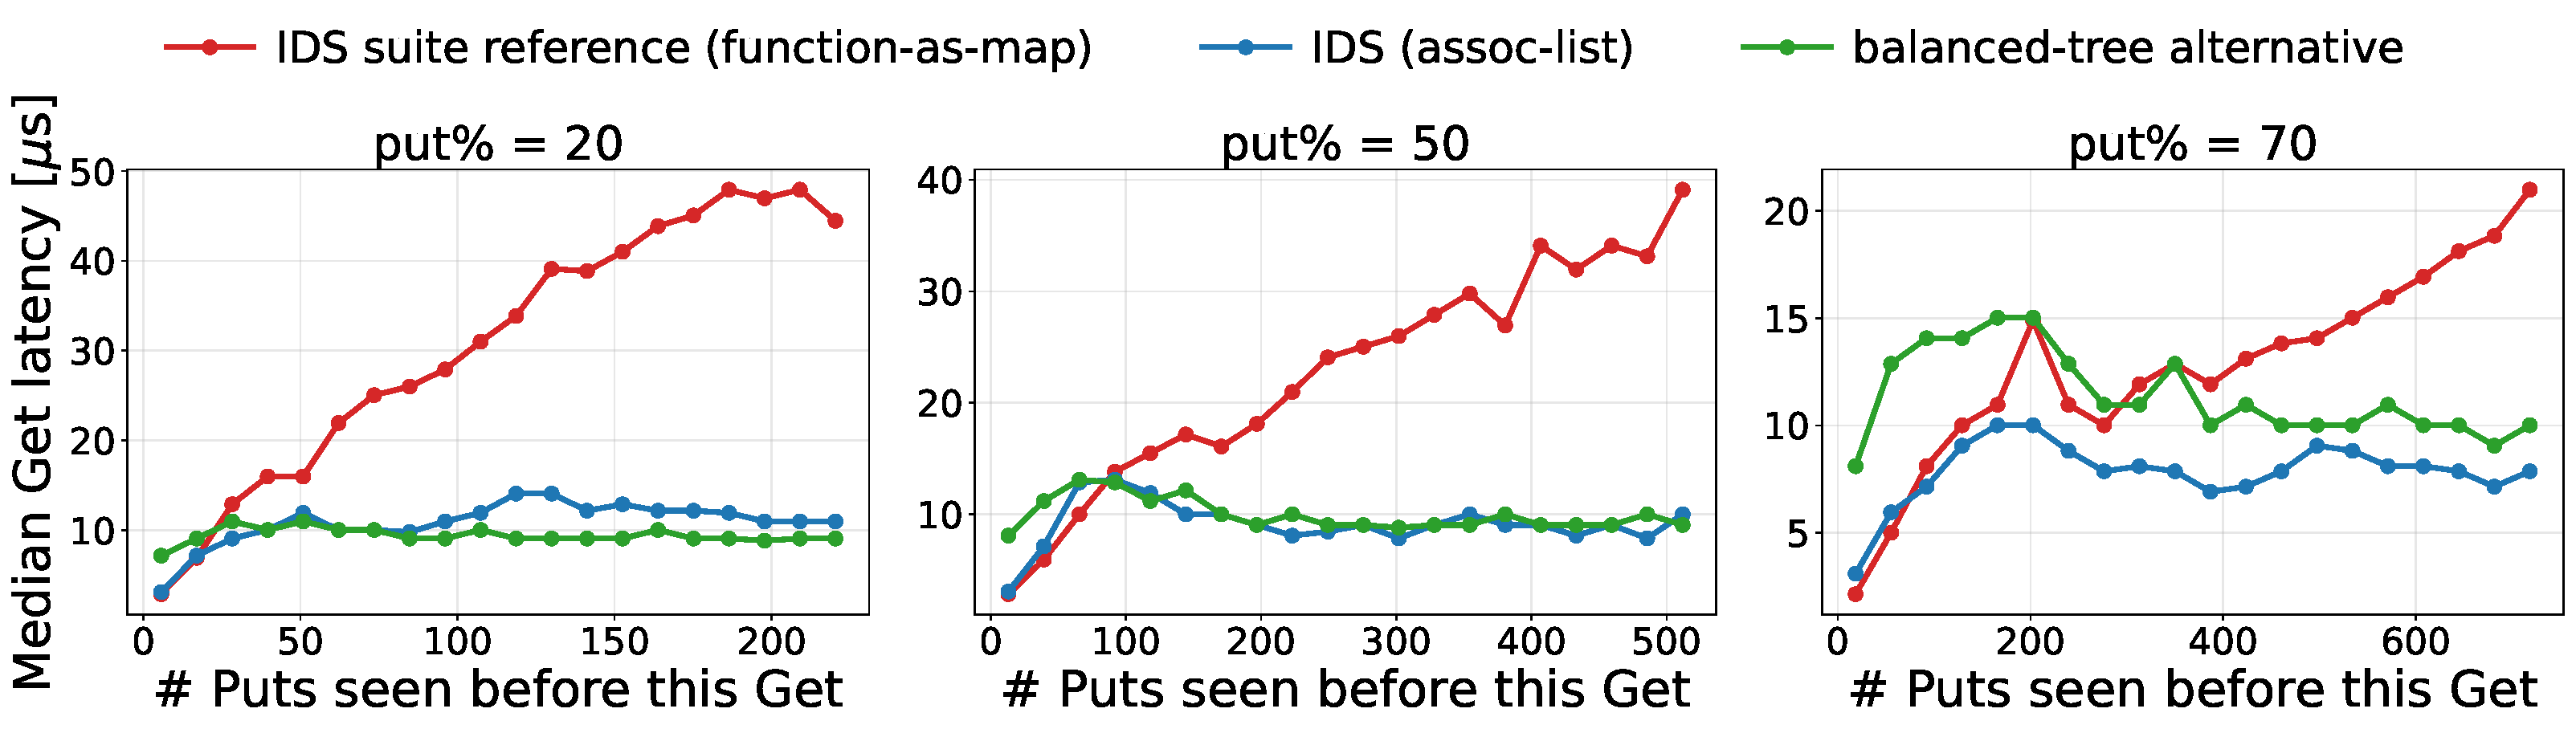
\includegraphics[width=\linewidth]{figures/figure_mr_get_vs_depth.pdf}
\caption{\texttt{Get} latency vs.\ closure depth (number of \texttt{Put}s preceding each \texttt{Get} in the same worker trace) for the three Monotonic Reads implementations at three put rates. The \sys{} suite reference's \texttt{Get} latency grows linearly with depth (slope $0.21\,\mu$s per closure layer at put $=20\%$, $R^2 = 0.95$). \sys{}' assoc-list slope is an order of magnitude smaller; the balanced-tree variant's slope is within statistical noise at every put rate.}
\label{fig:mr-depth}
\end{figure*}

\paragraph{Setup.}
Three MR implementations on the same runtime and identical wire format ($92.83$ B per \texttt{Put} on average): the \sys{} suite reference (function-as-map), \sys{} (assoc-list), and a balanced-tree alternative. Throughput differences are CPU-side. The balanced tree is a control: it tests whether \sys{}' win comes from the assoc-list specifically or from any structure that does not walk a closure chain on \texttt{Get}.

\paragraph{Where the cost lands.}
The reference pays on \texttt{Get}; the refinements pay on \texttt{Put}. At put $=50\%$:
\begin{center}
\begin{tabular}{lrr}
\toprule
implementation & $T_{\mathrm{get}}$ ($\mu$s) & $T_{\mathrm{put}}$ ($\mu$s) \\
\midrule
\sys{} suite reference (function-as-map) & $24.83$ & $15.40$ \\
\sys{} (assoc-list)                & $10.81$ & $16.81$ \\
balanced-tree alternative          & $11.40$ & $21.12$ \\
\bottomrule
\end{tabular}
\end{center}
Regressing \texttt{Get} latency against closure depth (number of \texttt{Put}s preceding a \texttt{Get} in the same worker trace) confirms the reference's chain walk: slope $0.21\,\mu$s/layer at put $=20\%$ ($R^2 = 0.95$, \cref{fig:mr-depth}). Both refinements stay flat across every put rate measured ($|\text{slope}| < 0.025\,\mu$s/layer): bounded data structure, no chain to walk. The balanced tree's extra Put cost comes from rebalance.

\paragraph{N-scaling at put $=50\%$.}
The reference's throughput drops as ops-per-worker $N$ grows; \sys{} stays nearly flat:
\begin{center}
\begin{tabular}{lrrrr}
\toprule
$N$ & $1{,}000$ & $2{,}000$ & $5{,}000$ & $20{,}000$ \\
\midrule
\sys{} suite reference (function-as-map) & $108{,}000$ & $100{,}000$ & $90{,}000$ & $80{,}000$ \\
\sys{} (assoc-list)                & $130{,}000$ & $124{,}000$ & $117{,}000$ & $112{,}000$ \\
\bottomrule
\end{tabular}
\end{center}
At $N=1{,}000$ \sys{} is $1.20\times$ faster; at $N=20{,}000$ the gap widens to $1.40\times$. Throughput drop from $N=1{,}000$ to $N=20{,}000$: reference $1.35\times$, \sys{} $1.16\times$. The reference's per-\texttt{Get} closure walk grows linearly with prior \texttt{Put}s, so its per-op cost rises with $N$; the assoc-list's lookup is bounded by the number of distinct keys in the workload (50 here), so its per-op cost is $N$-independent and only message-bus pressure causes the mild decline.


\newpage


\begin{figure*}[t]
\centering
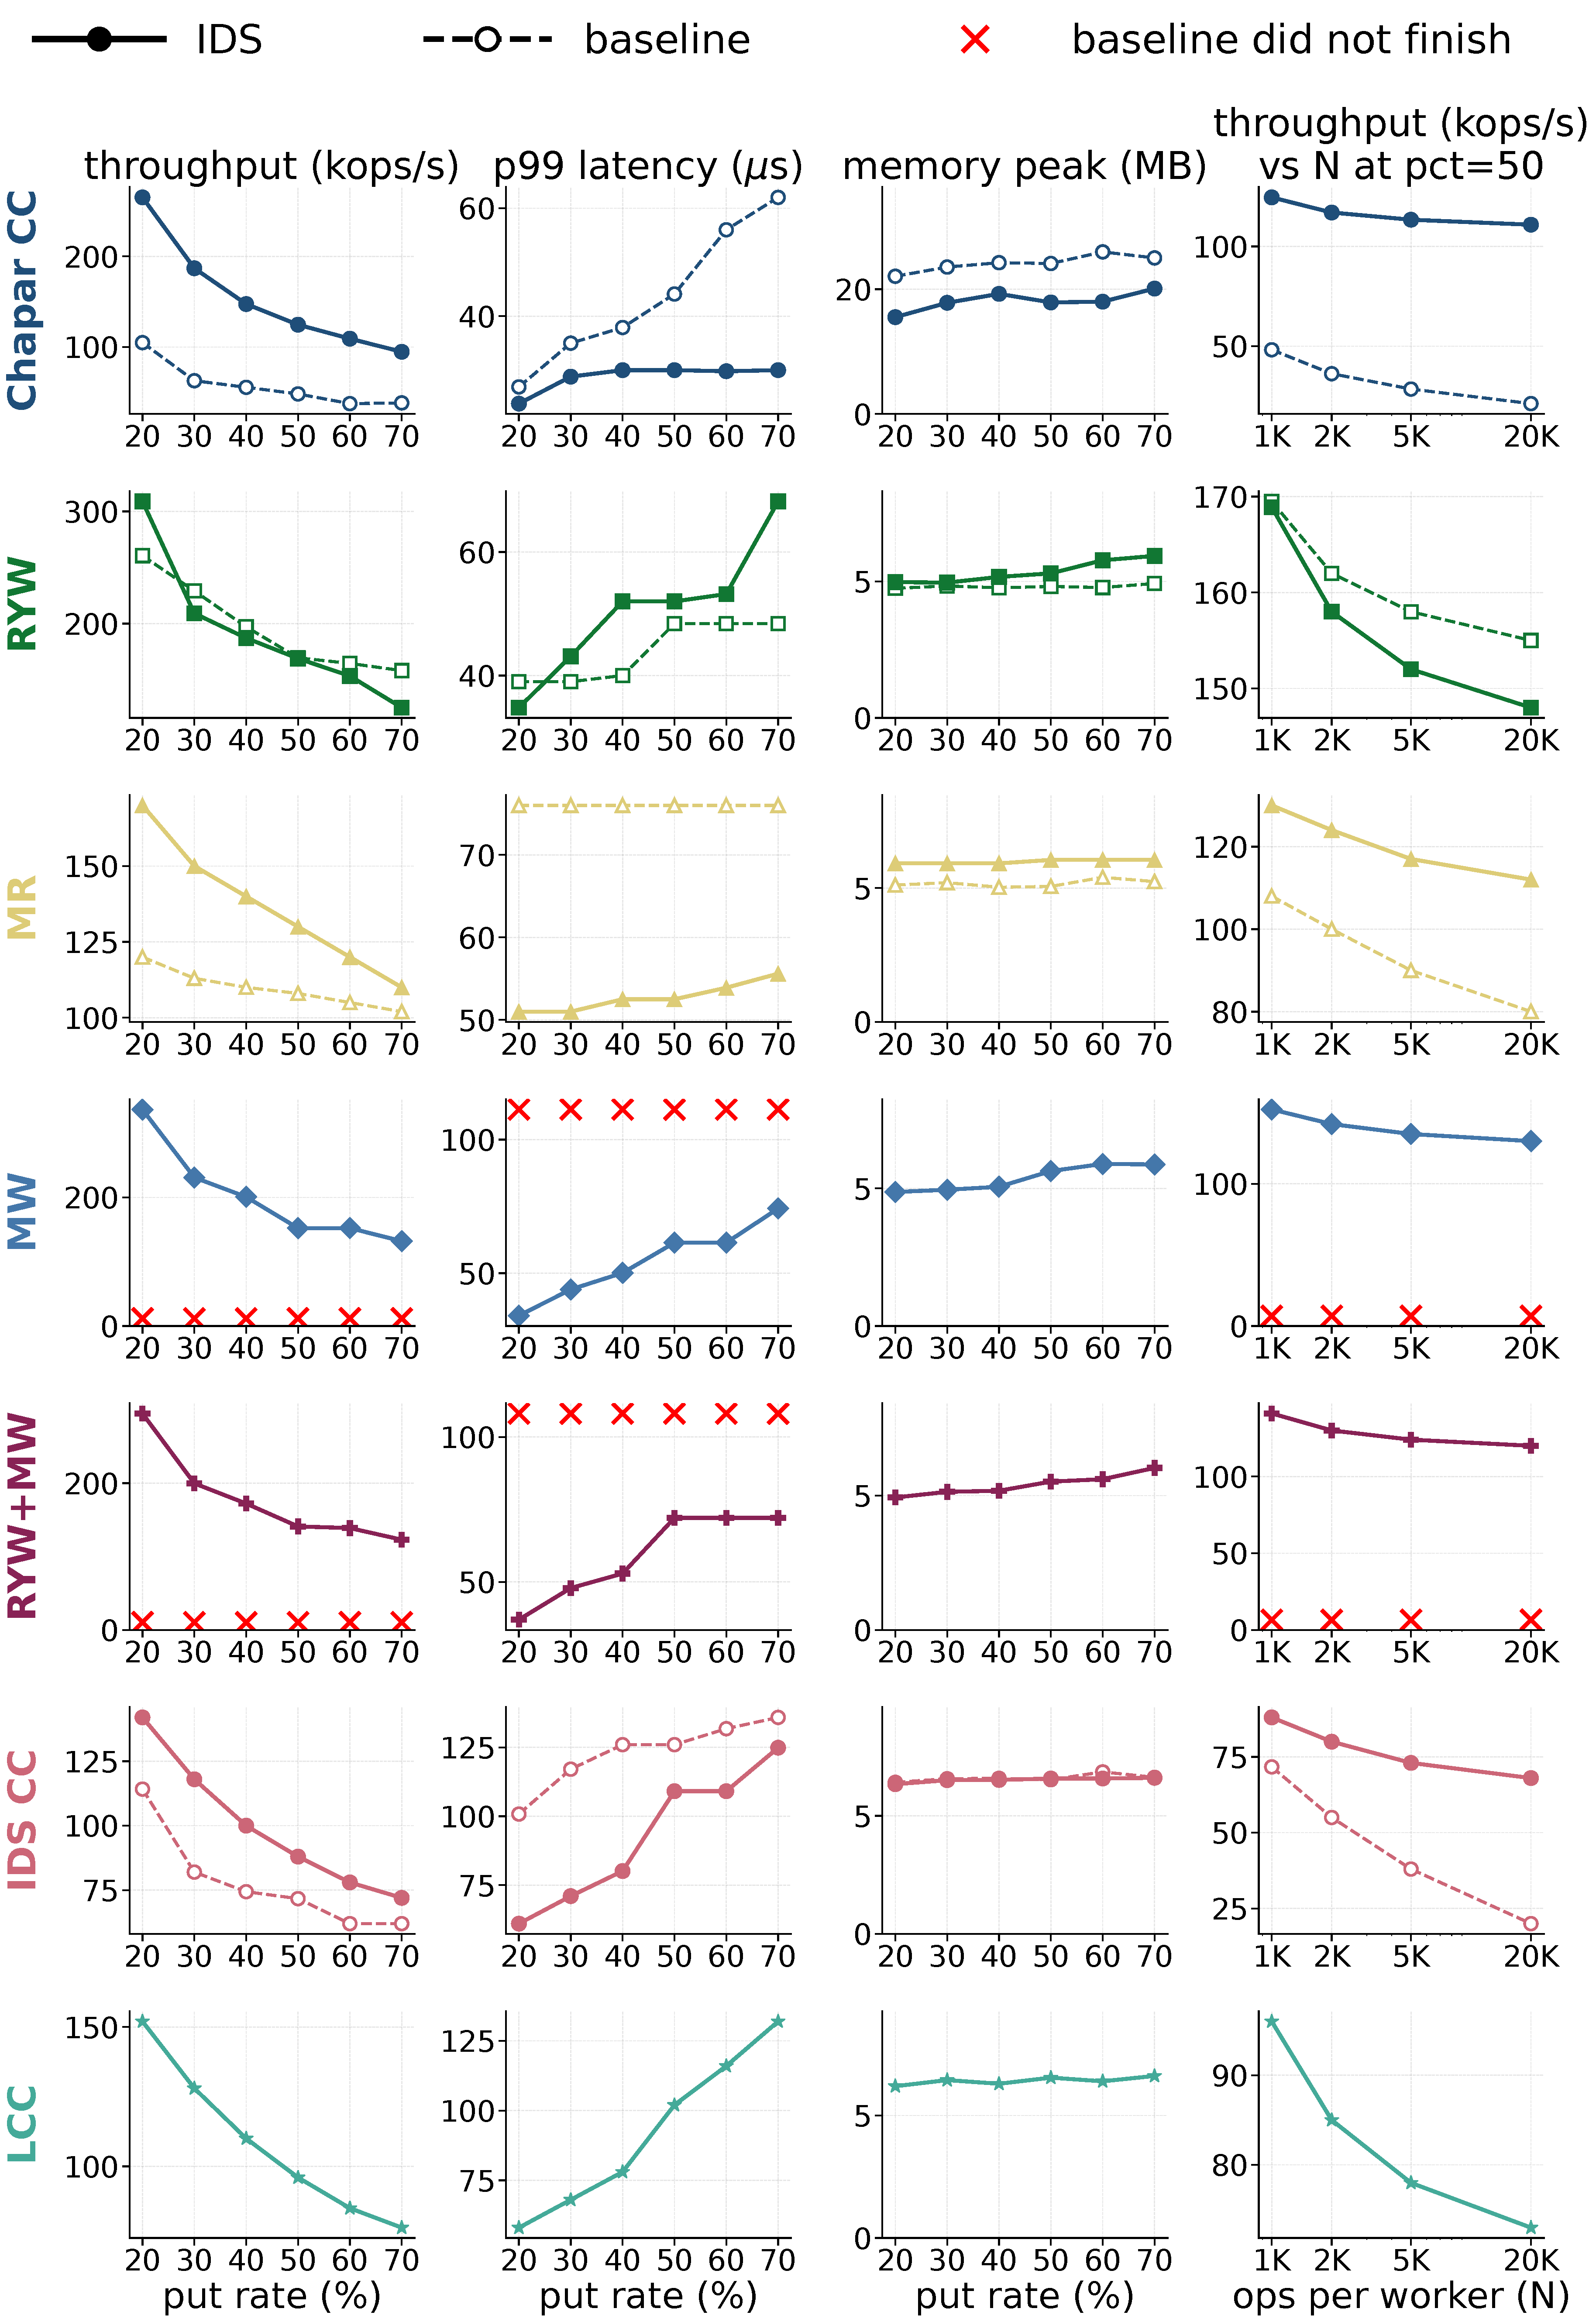
\includegraphics[width=\linewidth]{figures/eval_perf_appendix.pdf}
\caption{Per-protocol performance. Top row is Chapar CC (Chapar paper protocol) shown for comparison; the next five rows are the \sys{} suite specs (RYW, MR, MW, RYW+MW, \sys{} suite CC); the bottom LCC row is a single-line illustrative trajectory of labeled causal consistency. Columns: throughput (kops/s), p99 latency ($\mu$s), memory peak (MB), and throughput vs ops-per-worker $N$ at put $=50\%$. Per-protocol $y$-axes are dedicated so each row's range is visible. Solid $=$ \sys{}; dashed $=$ reference (function-as-map). Red $\times$ marks runs that hit the $180$\,s wall-clock cap; on MW and RYW+MW the reference times out at every put rate (the reference's read-then-write check on a function-as-map is the cause; see below).}
\label{fig:eval-perf-appendix}
\end{figure*}
   % E. Performance details
% \newpage
\section{Results on Proof, Annotation, and Code-and-Proof Benchmarks}
\label{app:benchmarks}

\sys{} beats every prior method on the four proof and annotation benchmarks, and reaches $\mathbf{176/189}$ on VERINA against prior SOTA $38$ and agentic baselines Codex $136$, Claude Code $149$ (\cref{tab:bench-results}).

\begin{table}[t]
\centering
\small
\setlength{\tabcolsep}{6pt}
\renewcommand{\arraystretch}{1.15}
\caption{What each cross-language benchmark gives the model and what the model must produce. \cmark{} = given as input; \xmark{} = the model must generate it. ``Spec'' covers preconditions and postconditions (or the theorem statement, where applicable). For DafnyBench the implementation body is given; only Dafny verification \emph{hints} (loop invariants, assertions, decreases clauses) are stripped. miniCodeProps and CoqStoq give the spec as a Lean / Coq theorem statement.}
\label{tab:bench-modalities}
\providecommand{\cmark}{\ding{51}}
\providecommand{\xmark}{\ding{55}}
\begin{tabular}{lllccccl}
\toprule
\multirow{2}{*}{Benchmark} & \multirow{2}{*}{Language} & \multirow{2}{*}{Verifier} & \multicolumn{4}{c}{Given to model} & \multirow{2}{*}{Task} \\
\cmidrule(lr){4-7}
& & & NL desc. & Signature & Spec & Code & \\
\midrule
DafnyBench~\cite{dafnybench}    & Dafny       & Dafny     & \xmark & \cmark & \cmark & \cmark & annotations \\
miniCodeProps~\cite{minicodeprops} & Lean 4   & Lean      & \xmark & \cmark & \cmark & \cmark & proof \\
Verus-Bench~\cite{autoverus}    & Rust        & Verus     & \xmark & \cmark & \cmark & \cmark & annotations \\
CoqStoq~\cite{rango}            & Coq         & Coq       & \xmark & \cmark & \cmark & \cmark & proof \\
CloverBench~\cite{clover}       & Dafny       & Dafny     & \cmark & \cmark & \cmark & \xmark & code + annot. \\
{VERINA}~\cite{verina}  & Lean 4 & Lean & \cmark & \cmark & \cmark & \xmark & \textbf{code + proof} \\
\bottomrule
\end{tabular}
\end{table}

\begin{table}[t]
\centering
\footnotesize
\setlength{\tabcolsep}{5pt}
\renewcommand{\arraystretch}{1.05}
\caption{Pass counts on verification benchmarks. Bold $=$ best per column. The first four are proof-only (impl and spec given); on these, \sys{} reduces to its DSA component since the ISA has no design space to search. The last three are concurrent code-and-proof tasks. Per-benchmark slices, prior-SOTA references, and CloverBench note in \cref{app:benchmarks}.}
\label{tab:bench-results}
\begin{tabular}{lccccccc}
\toprule
Method & DafnyBench & miniCodeProps & Verus-Bench & CoqStoq & VERINA & AlgoVeri & CloverBench \\
\midrule
Prior SOTA            & 52 / 100 & 49 / 100  & 137 / 150 & 28 / 100 & 38 / 189  & 31 / 77 & -- \\
Codex                 & 78 / 100 & 80 / 100  & 148 / 150 & 46 / 100 & 136 / 189 & 51 / 77 & 62 / 62 \\
Claude Code           & 76 / 100 & 86 / 100  & 148 / 150 & 51 / 100 & 149 / 189 & 56 / 77 & 62 / 62 \\
\midrule
\textbf{\sys{}} (ours) & \textbf{88 / 100} & \textbf{100 / 100} & 149 / 150 & \textbf{97 / 100} & \textbf{176 / 189} & \textbf{65 / 77} & 62 / 62 \\
\bottomrule
\end{tabular}
\end{table}


\subsection{Proof and annotation benchmarks}

\paragraph{Setup.}
The model receives a complete task specification (signature, preconditions, postconditions, and code where applicable) and must produce verifier-acceptable output: proof annotations on DafnyBench~\cite{dafnybench} and Verus-Bench~\cite{autoverus}, or a complete proof on miniCodeProps~\cite{minicodeprops} and CoqStoq~\cite{rango} (modality in \cref{tab:bench-modalities}). For each benchmark we use the slice the prior SOTA method published its number on:
\begin{itemize}
\item \textbf{DafnyBench}: $100$ hardest tasks; prior SOTA is DafnyPro~\cite{dafnypro} (from the DafnyBench paper).
\item \textbf{miniCodeProps}: $100$ tasks from the sorting split; prior SOTA is COPRA~\cite{copra}.
\item \textbf{Verus-Bench}: full $150$ tasks; prior SOTA is AutoVerus~\cite{autoverus}.
\item \textbf{CoqStoq}: $100$ hardest tasks; prior SOTA is Rango~\cite{rango}.
\end{itemize}

\paragraph{Result.}
\sys{} reaches $88/100$ on DafnyBench, $100/100$ on miniCodeProps, $149/150$ on Verus-Bench, and $97/100$ on CoqStoq (\cref{tab:bench-results}), beating the strongest prior on all four. The largest absolute gap is on CoqStoq ($+69$ over Rango); \sys{} hits a perfect $100/100$ on miniCodeProps, and on Verus-Bench all three LLM methods are within $1\%$ of saturation (\sys{} $149$, Codex $148$, Claude Code $148$ of $150$). Failures reflect per-task budget caps and proofs requiring tactics or library-specific lemmas the agent did not discover within budget (\cref{app:proof-method}).

\subsection{Code-and-proof benchmarks}

\paragraph{Setup.}
A second, recent line of benchmarks evaluates joint code-and-proof synthesis on single-function algorithmic tasks (sorting, search, list manipulation, basic arithmetic like factorial/gcd/Fibonacci): the model receives a natural-language description, signature, and spec, and produces both the code and a proof of correctness. These tasks are strictly simpler than the distributed-system specs of \cref{sec:eval-synthesis}: no concurrency, no replication, no multi-step operational semantics.
\begin{itemize}
\item \textbf{VERINA}~\cite{verina}: $189$ Lean tasks; prior SOTA is iterative refinement with Lean compiler feedback ($64$ rounds), reported in the VERINA paper.
\item \textbf{AlgoVeri}~\cite{algoveri}: $77$ problems, each expressed in Dafny, Verus, and Lean; prior SOTA $31/77$ (Gemini-3 Flash, Dafny track, reported in the AlgoVeri paper).
\item \textbf{CloverBench}~\cite{clover}: $62$ Dafny tasks. We omit a Prior-SOTA cell because Clover (the only prior published method) evaluates a different task: its consistency-checker filters pre-existing correct triples (an $87\%$ acceptance rate, with $13\%$ false negatives where it rejects a known-correct triple). Our column reports end-to-end synthesis: given the spec, the model generates code and annotations, and the Dafny verifier accepts.
\end{itemize}

\paragraph{Result.}
\sys{} reaches $\mathbf{176/189}$ on VERINA, well above prior SOTA $38$ and agentic baselines Codex $136$, Claude Code $149$; $\mathbf{65/77}$ on AlgoVeri's Dafny track, $2\times$ the published Gemini-3 Flash baseline of $31/77$; and all three LLM methods saturate at $62/62$ on CloverBench.
    % F. Cross-language + concurrent benchmark details
\section{\sys{} Architecture Details}
\label{app:architecture}

This appendix expands on the components introduced in \cref{sec:design} and ablated in \cref{sec:eval-ablations}. The architecture instantiates the two-level CEGIS-style refinement of \cref{sec:design}. The inner loop is the DSA (\cref{app:worker}): forward moves \emph{Define}, \emph{Prove}, \emph{Decompose} extend the partial (code, proof) candidate, and the structured \coq{} diagnostic from a failed step (\cref{app:feedback}) is a concrete witness that the candidate cannot close as written, used by the agent to choose \emph{Repair} or \emph{Revert}. The outer loop is the ISA: a DSA's stalled proof attempts and bench failures (\cref{app:bench-signal}) drive the proposer (\cref{app:guide}) on tactical stalls and the reloader (\cref{app:resetter}) on strategic dead-ends. The audit step (\cref{app:auditor}) is orthogonal to refinement: it is a deterministic safety gate, not a counterexample signal.

\providecolor{specbg}{HTML}{F7F8FA}
\providecolor{specrule}{HTML}{C8CDD3}
\providecommand{\promptbox}[1]{%
  {\setlength{\fboxsep}{6pt}\setlength{\fboxrule}{0.3pt}%
   \noindent\fcolorbox{specrule}{specbg}{\begin{minipage}{0.96\linewidth}\small #1\end{minipage}}}%
}

\subsection{Proof methodology}
\label{app:proof-method}

Each spec is a \coq{} \texttt{Module Type} carrying a \texttt{State} type, an \texttt{Update} type, seven method signatures (\texttt{getReq}, \texttt{getGuard}, \texttt{get}, \texttt{getRes}, \texttt{putReq}, \texttt{putGuard}, \texttt{put}), and an operational semantics on client--replica configurations. The implementation \sys{} produces is an \texttt{AlgDef} module providing the same seven methods at concrete state types, plus a \texttt{Refinement} module proving forward simulation: every step the implementation can take corresponds to a step the abstract spec can take, on related states. From the \texttt{Refinement} we obtain a \texttt{TraceInclusion} theorem: every observable trace of the implementation is also a trace of the abstract spec.

The tactic vocabulary is standard \coq{}: \texttt{inversion}, \texttt{destruct}, \texttt{subst}, \texttt{rewrite}, \texttt{apply}, \texttt{econstructor; eauto}, \texttt{simpl}, \texttt{lia}, \texttt{congruence}, with case-analysis on \texttt{Nat.eq\_dec} for equality decisions on identifiers and timestamps. No \texttt{firstorder}/\texttt{intuition} shortcuts; no \texttt{Admitted}, no \texttt{Axiom}, no \texttt{Hypothesis}, no \texttt{Parameter}. Closure is verified by \coq{}'s kernel.

\subsection{DSA: deductive synthesis}
\label{app:worker}

The DSA is a Codex (or Claude Code) session per workspace performing the deductive-synthesis loop of \cref{sec:design-worker}. At each search-tree node the agent moves forward with one of three primitives:
\begin{itemize}[leftmargin=*,itemsep=2pt,topsep=2pt]
\item \emph{Define}: declare or extend a state/message type or function body, with \texttt{admit} placeholders for parts not yet filled in (e.g.\ adding a \texttt{Cell} record to the per-key store with \texttt{cell\_deps} stubbed).
\item \emph{Prove}: close an open proof obligation by replacing \texttt{Admitted} with a tactic sequence ending in \texttt{Qed}, or extend an existing tactic block.
\item \emph{Decompose}: state a helper lemma as \texttt{Admitted} and use it to advance the proof of an existing lemma; the helper is discharged in a later iteration.
\end{itemize}

After each forward step \texttt{make} runs and \coq{}'s type-checker is the only oracle. On error, the agent backtracks with one of two primitives:
\begin{itemize}[leftmargin=*,itemsep=2pt,topsep=2pt]
\item \emph{Repair}: re-attempt the failed step with a different tactic (e.g.\ \texttt{induction} instead of \texttt{destruct}; \texttt{lia} instead of \texttt{omega}).
\item \emph{Revert}: rewind to an earlier search-tree node and choose a different forward primitive (typically when the same compile error recurs three or more times).
\end{itemize}

The agent's initial brief is read from \texttt{CLAUDE.md} in the workspace and instantiates the four briefings of \cref{sec:design-worker} (methodology, auditability, design, tactical playbook). The brief shown below is for the \coq{} setting (our \sys{} suite specs and Chapar CC, plus CoqStoq and miniCodeProps); for cross-language benchmarks we swap the verifier and surface tools to match the target language: Dafny (DafnyBench, AlgoVeri-Dafny, CloverBench), Verus (Verus-Bench), and Lean~4 (VERINA), with success criterion adapted accordingly (e.g.\ \texttt{dafny verify} accepts, \texttt{lake build} succeeds, \texttt{verus} reports zero errors).

\promptbox{%
\textbf{Role: Deductive Synthesis Agent.} Given a specification, incrementally produce an implementation and a machine-checked proof that it satisfies the specification. The type-checker is the only oracle and accepts a partial state (with deferred holes) as a valid intermediate.

\textbf{Schema.} Synthesis is a finite sequence of well-typed steps; the file must type-check (possibly with deferred holes) after every step. Take one forward move:
\begin{itemize}[leftmargin=1.4em,itemsep=1pt,topsep=1pt]
\item \emph{Define} (refinement): introduce or extend a \texttt{Definition}, \texttt{Record}, \texttt{Inductive}, \texttt{Fixpoint}, or \texttt{Module}; bodies may contain \texttt{admit} or invoke \texttt{Admitted} lemmas.
\item \emph{Prove} (closure): replace an \texttt{Admitted} lemma with a tactic sequence ending in \texttt{Qed}, or extend an existing partial proof.
\item \emph{Decompose} (lemma introduction): state a helper lemma as \texttt{Admitted}, use it to advance the current proof, and discharge it later. This is the deferred-hole device of deductive synthesis.
\end{itemize}
On error, backtrack: \emph{Repair} (different tactic on the same goal, e.g.\ \texttt{induction} instead of \texttt{destruct}, \texttt{lia} instead of \texttt{omega}) or \emph{Revert} (rewind to an earlier state and try a different forward move; trigger when the same error recurs three or more times).

\textbf{Invariants.} (I1)~The file type-checks after every step. (I2)~Every \texttt{Admitted} is a deferred hole, not a permanent assumption: all \texttt{Admitted} must be closed before reporting \emph{done}. (I3)~The specification is fixed. (I4)~No \texttt{Axiom}, \texttt{Hypothesis}, \texttt{Parameter}, or unguarded recursion.

\textbf{Design.} State types should be concrete (records, bounded lists, indexed nats), not function types whose \texttt{override} builds closure chains under repeated update. State must not grow unboundedly with the number of operations: traces, logs, and accumulated dependency lists belong in the proof context, not the runtime state.

\textbf{Termination.} Report \emph{done} when (a)~the file type-checks with zero \texttt{Admitted} and zero \texttt{admit}, and (b)~the audit step passes (no vacuous proofs; no specification edits; non-trivial method bodies). The coordinator additionally extracts the implementation and runs the benchmark harness; if extraction or execution fails, the run reverts.

\textbf{Tactical playbook.}
\begin{itemize}[leftmargin=1.4em,itemsep=1pt,topsep=1pt]
\item Build simple to complex: prove small structural facts first, then combine.
\item When stuck on a subgoal, read it carefully; the goal often names the missing helper.
\item Use \texttt{admit} (lowercase) to skip subgoals temporarily; the final file must have zero \texttt{Admitted} and zero \texttt{admit}.
\end{itemize}
}

\cref{app:progression} walks through an end-to-end illustration of this schema on a small target (\texttt{all\_less\_than}): each of the five synthesis steps is annotated with its move (\emph{Define}, \emph{Prove}, \emph{Decompose}), with every intermediate listing type-checking under the kernel.

\subsection{Audit step}
\label{app:auditor}

The audit step is a deterministic Python script that gates closure with kernel-level verdicts (no model outputs). It encapsulates the cheating patterns we have observed during runs.

\textbf{Static checks.}
\begin{itemize}[leftmargin=*,itemsep=2pt,topsep=2pt]
\item \texttt{Admitted} count is zero.
\item After stripping comments, \texttt{Axiom}, \texttt{Hypothesis}, and \texttt{Parameter} counts are zero.
\item \texttt{make clean \&\& make} exits zero.
\end{itemize}

\textbf{Vacuous-proof patterns.} The script also matches the closed file against four patterns:
\begin{itemize}[leftmargin=*,itemsep=2pt,topsep=2pt]
\item A \texttt{put} that returns a fixed constant the spec accepts on every input.
\item An always-true \texttt{getGuard} that admits any read.
\item A forward-simulation theorem stated over an empty domain so that it holds vacuously.
\item A state-only stub whose \texttt{Update} drops the payload and returns the initial state on every operation.
\end{itemize}

A candidate that fails any check is sent to the ISA; only candidates passing all checks count as audit-clean closures.

\subsection{Proposer (ISA tactical role)}
\label{app:guide}

After the coordinator counts no progress across $10$ consecutive polls, the proposer fires as a one-shot LLM session. It receives the work file, every \texttt{Admitted} lemma's surrounding $17$-line context, and the most recent \texttt{make} error with $4$ lines of trailing context when present, and writes its output to \texttt{GUIDANCE.md} in the workspace.

\promptbox{%
\textbf{Role.} You are an expert \coq{} proof advisor. Read the work file and focus on the proof goals and error context below. Do NOT edit the \texttt{.v} file.

\textbf{For each Admitted proof, follow this checklist:}
\begin{enumerate}[leftmargin=1.4em,itemsep=1pt,topsep=1pt]
\item \textbf{Read the lemma statement.} What does it claim? What are the hypotheses? What is the conclusion type?
\item \textbf{Identify the proof structure needed:}
\texttt{forall x, P x} $\to$ \texttt{intros x};
inductive type (list, trace, nat) $\to$ \texttt{induction} on it;
step/transition $\to$ \texttt{destruct} on the step type, then case analysis;
simulation $\to$ invariant + induction on trace length;
two functions equal $\to$ \texttt{functional\_extensionality}.
\item \textbf{Identify missing helper lemmas.} For each subgoal you cannot close directly, state the EXACT helper (name, signature, informal meaning). Suggest: prove it separately; \texttt{Admit} it in the main proof; close it.
\item \textbf{If the proof is $>30$ lines, decompose:} by cases (\texttt{X\_case\_C1}, \texttt{X\_case\_C2}, \dots\ for each constructor); by subgoal (if $A \wedge B$, prove $A$ and $B$ separately); extract common patterns repeating $3$+ times.
\item \textbf{Suggest specific tactic sequences,} not vague directions.
\end{enumerate}

\textbf{For compile errors,} diagnose using a decision tree (e.g., \emph{``Cannot unify X with Y''} $\to$ type mismatch, use \texttt{Check expr.}; \emph{``Tactic failure''} $\to$ try \texttt{lia} instead of \texttt{omega}; \emph{``No matching clauses''} $\to$ incomplete pattern match).

\textbf{Output.} Write \texttt{GUIDANCE.md} with one section per Admitted proof or error: (a) the diagnosis, (b) the exact tactic sequence to try, (c) any helper-lemma signatures.
}

On Chapar, the proposer chose three sub-lemma classes (per-message, per-store-entry, per-replica-clock) by recognising that the global delivery invariant decomposes cleanly along these axes, none of which \coq{}'s automation closes alone.

\subsection{Reloader (ISA strategic role)}
\label{app:resetter}

The reloader escalates every $20$ polling cycles when no progress is detected: Level $1$ at stall cycle $20$, Level $2$ at $40$, Level $3$ at $60$, and so on. Each level is a one-shot LLM session reading \texttt{DESIGN\_LOG.md}, \texttt{STATUS.md}, and every prior level's output, and writes \texttt{META\_GUIDANCE\_L\{N\}.md}. The strategist consumes the output to rewrite its plan and spawn a fresh worker on the new design.

\promptbox{%
\textbf{Role.} You are a level-$N$ formal verification architect. Read \texttt{DESIGN\_LOG.md}, \texttt{STATUS.md}, and every prior \texttt{META\_GUIDANCE\_L\{1..N{-}1\}.md}: the history of all approaches tried and why each failed.

\textbf{Synthesize a NEW approach that avoids ALL recorded failures.} Think across these dimensions:
\begin{enumerate}[leftmargin=1.4em,itemsep=1pt,topsep=1pt]
\item \textbf{Data representation.} Concrete types for state and messages: records, bounded lists, nats, not functions.
\item \textbf{Abstraction function.} How concrete state maps to abstract state. This is the KEY creative choice; if previous attempts failed on the simulation proof, the abstraction was wrong.
\item \textbf{Invariant.} What property holds at every reachable state. The invariant must be (a)~true initially, (b)~preserved by every step, (c)~strong enough to prove the final theorem.
\item \textbf{Proof decomposition.} Which helper lemmas are needed, stated explicitly with signatures.
\item \textbf{Minimum information.} For each function that takes a collection, could the caller pass a smaller collection and still get a correct result? The most precise design passes only what is needed per call.
\end{enumerate}

\textbf{Output.} Write \texttt{META\_GUIDANCE\_L\{N\}.md} as a CONCRETE blueprint a worker can directly implement: exact \texttt{Record} types, method signatures, abstraction function, invariant, and lemma decomposition. Do NOT write vague advice; do NOT spawn workers.
}

On Chapar, the reloader chose a per-key store entry recording sender, sender clock, and dependency vector; alternative layouts (e.g.\ a single global per-replica state) leave the delivery lemma unprovable from local information.

\subsection{\coq{} feedback}
\label{app:feedback}

Each \texttt{make} invocation captures stdout/stderr; on non-zero exit, the coordinator extracts every \texttt{Error:} line plus $2$ lines of preceding context and $4$ lines of trailing context as a single error block. The block is included verbatim in the worker's next prompt alongside the proof goal, the local hypothesis context, and the tactic backtrace where applicable. No normalisation or summarisation is applied: the structured \coq{} diagnostic carries the localisation signal. Replacing this stream with a binary accept/reject collapses the search (\cref{sec:eval-ablations} reports $\le 1/3$ closure on every \coq{} spec under $-$VF).

\subsection{Performance feedback}
\label{app:bench-signal}

When a worker reaches a verifier-clean state with a design hash distinct from prior runs, the coordinator invokes the benchmark harness asynchronously. The harness extracts the implementation to OCaml, deploys it on the cluster (\cref{app:perf-harness}), and writes results to \texttt{PERF\_RESULTS.md} in the workspace. Throughput targets are calibrated per-spec from the published reference; implementations whose throughput falls below the target are flagged and trigger the reloader on the next escalation.
  % B. Architecture details
\section{Synthesis Progression: \texttt{all\_less\_than}}
\label{app:progression}

% [addressed: each step compiles in Rocq 9.1; intermediate stubs use Parameter (compilable) instead of literal `todo` (not Coq); rejected else-branch attempt verified to actually fail] \ak{we should run the synthesis for this spec and use its output, this is using the manual output stages}

This appendix walks through one full progression of \sys{}' deductive-synthesis loop on a small target. Step~0 and the Final State are complete \coq{} files that compile; the listings for intermediate Steps~1--5 show only the parts that change from the previous step, with not-yet-filled bodies stubbed as \texttt{Parameter}. The progression on real distributed-system specs follows the same pattern at much larger scale (\cref{sec:eval-synthesis}); the small target keeps each listing short enough to read end-to-end.

The five synthesis steps below are an instance of the deductive-synthesis schema of \cref{app:worker}. Step 1 is a \emph{Decompose} (split the goal into a \texttt{nil} and a \texttt{cons} helper lemma). Step 2 combines \emph{Define} (fill the \texttt{nil} body) with \emph{Prove} (close the \texttt{nil} helper). Step 3 is another \emph{Decompose} (split the \texttt{cons} helper on the head). Step 4 is \emph{Define} (the recursive call). Step 5 combines \emph{Define} (fill the \texttt{else} branch) with \emph{Prove} (close the \texttt{else} helper). The file type-checks at every step (Invariant I1); \texttt{Admitted} placeholders carry the deferred holes forward and are all discharged by the Final state.

The target is \texttt{all\_less\_than : list nat -> nat -> bool}, returning \texttt{true} iff every element of the input list is strictly less than the bound \texttt{n}. The correctness statement is the iff-equivalence with \texttt{Forall}:
\begin{quote}
  \texttt{all\_less\_than l n = true} $\Leftrightarrow$ \texttt{Forall (fun x => x < n) l}.
\end{quote}

\subsection{Step 0: bare specification}
The implementation is a \texttt{Parameter}; the correctness lemma is \texttt{Admitted}. The file type-checks but proves nothing.

\begin{lstlisting}[label={lst:state0}, caption={Step 0: spec only.}]
Require Import Coq.Lists.List.

Parameter all_less_than : list nat -> nat -> bool.

Lemma all_less_than_correct : forall (l : list nat) (n : nat),
  all_less_than l n = true <-> Forall (fun x => x < n) l.
Proof.
Admitted.
\end{lstlisting}

\subsection{Step 1: case-split on the input list}
The agent commits to recursing on \texttt{l}. The implementation becomes a \texttt{Definition} with a \texttt{match} on \texttt{nil}/\texttt{cons}; the branch bodies are stubbed as \texttt{Parameter}s. The correctness lemma is split into a \texttt{\_nil} helper and a \texttt{\_cons} helper, both \texttt{Admitted}; the main lemma now closes by \texttt{induction} on \texttt{l}, applying each helper at its leaf.

\begin{lstlisting}
Parameter nil_body : bool.
Parameter cons_body : nat -> list nat -> bool.

Definition all_less_than (l : list nat) (n : nat) : bool :=
  match l with
  | nil => nil_body
  | x :: xs => cons_body x xs
  end.

Lemma all_less_than_correct_nil : forall (n : nat),
  all_less_than nil n = true <-> Forall (fun x => x < n) nil.
Proof. Admitted.

Lemma all_less_than_correct_cons :
  forall (x : nat) (xs : list nat) (n : nat),
  all_less_than (x :: xs) n = true <-> Forall (fun x => x < n) (x :: xs).
Proof. Admitted.

Lemma all_less_than_correct : forall (l : list nat) (n : nat),
  all_less_than l n = true <-> Forall (fun x => x < n) l.
Proof.
  intros l n. induction l as [| x xs IH].
  - apply all_less_than_correct_nil.
  - apply all_less_than_correct_cons.
Qed.
\end{lstlisting}

\subsection{Step 2: fill the \texttt{nil} branch and close the \texttt{nil} helper}
The agent fills \texttt{nil\_body} with \texttt{true} (replacing the \texttt{Parameter}) and proves \texttt{\_nil}: both sides of the iff are vacuously satisfied (\texttt{true = true}; \texttt{Forall \_ nil} holds by the empty constructor). The \texttt{cons} body is still a \texttt{Parameter}.

\begin{lstlisting}
Definition all_less_than (l : list nat) (n : nat) : bool :=
  match l with
  | nil => true
  | x :: xs => cons_body x xs
  end.

Lemma all_less_than_correct_nil : forall (n : nat),
  all_less_than nil n = true <-> Forall (fun x => x < n) nil.
Proof. intros. simpl. split; intros; constructor. Qed.
\end{lstlisting}

\subsection{Step 3: introduce the \texttt{if} branch and split the \texttt{cons} helper}
The agent commits to comparing \texttt{x} against \texttt{n} via \texttt{x <? n}, leaving both branches as \texttt{Parameter} stubs. The \texttt{\_cons} helper is split into a \texttt{\_then} sub-helper (under \texttt{x < n}) and an \texttt{\_else} sub-helper (under \texttt{$\neg$(x < n)}), and \texttt{\_cons} now proves itself by case-splitting on \texttt{Nat.ltb\_spec} and applying the appropriate sub-helper.

\begin{lstlisting}
Parameter then_body else_body : nat -> list nat -> nat -> bool.

Definition all_less_than (l : list nat) (n : nat) : bool :=
  match l with
  | nil => true
  | x :: xs => if x <? n then then_body x xs n else else_body x xs n
  end.

Lemma all_less_than_correct_cons_then :
  forall (x : nat) (xs : list nat) (n : nat),
  x < n -> (all_less_than xs n = true <-> Forall (fun x => x < n) xs) ->
  (all_less_than (x :: xs) n = true <-> Forall (fun x => x < n) (x :: xs)).
Proof. Admitted.

Lemma all_less_than_correct_cons_else :
  forall (x : nat) (xs : list nat) (n : nat),
  ~ (x < n) -> (all_less_than xs n = true <-> Forall (fun x => x < n) xs) ->
  (all_less_than (x :: xs) n = true <-> Forall (fun x => x < n) (x :: xs)).
Proof. Admitted.

Lemma all_less_than_correct_cons :
  forall (x : nat) (xs : list nat) (n : nat),
  all_less_than xs n = true <-> Forall (fun x => x < n) xs ->
  all_less_than (x :: xs) n = true <-> Forall (fun x => x < n) (x :: xs).
Proof.
  intros. destruct (Nat.ltb_spec x n) as [Hlt | Hge].
  - apply all_less_than_correct_cons_then; assumption.
  - apply all_less_than_correct_cons_else; [apply Nat.le_ngt; assumption | assumption].
Qed.
\end{lstlisting}

\subsection{Step 4: fill the \texttt{then} branch with the recursive call}
The agent fills \texttt{then\_body} with \texttt{all\_less\_than xs n}: the implementation now actually recurses, so \texttt{Definition} is promoted to \texttt{Fixpoint}. The \texttt{\_then} helper proves cleanly: under \texttt{x < n}, applying \texttt{Nat.ltb\_lt} rewrites the \texttt{if}-condition to \texttt{true}, and \texttt{Forall} on \texttt{x :: xs} reduces to \texttt{x < n} on the head plus \texttt{Forall} on \texttt{xs}, both available.

\begin{lstlisting}
Fixpoint all_less_than (l : list nat) (n : nat) : bool :=
  match l with
  | nil => true
  | x :: xs => if x <? n then all_less_than xs n else else_body x xs n
  end.

Lemma all_less_than_correct_cons_then :
  forall (x : nat) (xs : list nat) (n : nat),
  x < n -> (all_less_than xs n = true <-> Forall (fun x => x < n) xs) ->
  (all_less_than (x :: xs) n = true <-> Forall (fun x => x < n) (x :: xs)).
Proof.
  intros x xs n Hlt H_ind. simpl.
  apply Nat.ltb_lt in Hlt. rewrite Hlt.
  split; intros.
  - constructor; [apply Nat.ltb_lt; assumption | tauto].
  - inversion H. tauto.
Qed.
\end{lstlisting}

\subsection{Step 5: fill the \texttt{else} branch and close the \texttt{else} helper}
The agent's first attempt is to recurse: \texttt{else\_body := all\_less\_than xs n} (``skip the out-of-bound element, keep checking''). The implementation type-checks, but the \texttt{\_else} obligation does not: under $\neg(x < n)$ the goal becomes \texttt{all\_less\_than xs n = true} $\Leftrightarrow$ \texttt{Forall (fun y => y < n) (x :: xs)}, which fails on \texttt{xs = nil}, \texttt{x = 5}, \texttt{n = 3} (LHS is \texttt{true}; RHS demands \texttt{5 < 3}). \coq{} rejects the proof. The agent backtracks and replaces the \texttt{else} body with \texttt{false}: the function now returns false on any out-of-bound element, the \texttt{\_else} helper closes (LHS becomes \texttt{false = true}, closed by \texttt{discriminate}; RHS gives \texttt{x < n} from inversion of \texttt{Forall}, contradicting $\neg(x < n)$).

\begin{lstlisting}
(* Attempt 1: else_body := all_less_than xs n  (rejected: iff fails) *)
(* Attempt 2: else_body := false               (accepted)            *)

Lemma all_less_than_correct_cons_else :
  forall (x : nat) (xs : list nat) (n : nat),
  ~ (x < n) -> (all_less_than xs n = true <-> Forall (fun x => x < n) xs) ->
  (all_less_than (x :: xs) n = true <-> Forall (fun x => x < n) (x :: xs)).
Proof.
  intros x xs n Hge _. simpl.
  apply Nat.le_ngt in Hge. apply Nat.ltb_ge in Hge. rewrite Hge.
  split.
  - discriminate.
  - intros HF. inversion HF; subst.
    apply Nat.ltb_lt in H1. congruence.
Qed.
\end{lstlisting}

\subsection{Final state}

After five steps every \texttt{Parameter} stub and \texttt{Admitted} placeholder is closed. \coq{}'s kernel accepts the file, verifying \texttt{all\_less\_than\_correct} on every input.

\begin{lstlisting}[label={lst:state5}, caption={Step 5 (final): implementation and proof, fully verified.}]
Require Import Coq.Lists.List.
Require Import Coq.Arith.PeanoNat.

Fixpoint all_less_than (l : list nat) (n : nat) : bool :=
  match l with
  | nil => true
  | x :: xs => if x <? n then all_less_than xs n else false
  end.

Lemma all_less_than_correct_nil : forall (n : nat),
  all_less_than nil n = true <-> Forall (fun x => x < n) nil.
Proof. intros. simpl. split; intros; constructor. Qed.

Lemma all_less_than_correct_cons_then :
  forall (x : nat) (xs : list nat) (n : nat),
  x < n -> (all_less_than xs n = true <-> Forall (fun x => x < n) xs) ->
  (all_less_than (x :: xs) n = true <-> Forall (fun x => x < n) (x :: xs)).
Proof.
  intros x xs n Hlt H_ind. simpl.
  apply Nat.ltb_lt in Hlt. rewrite Hlt.
  split; intros.
  - constructor; [apply Nat.ltb_lt; assumption | tauto].
  - inversion H. tauto.
Qed.

Lemma all_less_than_correct_cons_else :
  forall (x : nat) (xs : list nat) (n : nat),
  ~ (x < n) -> (all_less_than xs n = true <-> Forall (fun x => x < n) xs) ->
  (all_less_than (x :: xs) n = true <-> Forall (fun x => x < n) (x :: xs)).
Proof.
  intros x xs n Hge _. simpl.
  apply Nat.le_ngt in Hge. apply Nat.ltb_ge in Hge. rewrite Hge.
  split.
  - discriminate.
  - intros HF. inversion HF; subst.
    apply Nat.ltb_lt in H1. congruence.
Qed.

Lemma all_less_than_correct_cons :
  forall (x : nat) (xs : list nat) (n : nat),
  all_less_than xs n = true <-> Forall (fun x => x < n) xs ->
  all_less_than (x :: xs) n = true <-> Forall (fun x => x < n) (x :: xs).
Proof.
  intros. destruct (Nat.ltb_spec x n) as [Hlt | Hge].
  - apply all_less_than_correct_cons_then; assumption.
  - apply all_less_than_correct_cons_else; [apply Nat.le_ngt; assumption | assumption].
Qed.

Lemma all_less_than_correct : forall (l : list nat) (n : nat),
  all_less_than l n = true <-> Forall (fun x => x < n) l.
Proof.
  intros l n. induction l as [| x xs IH].
  - apply all_less_than_correct_nil.
  - apply all_less_than_correct_cons. assumption.
Qed.
\end{lstlisting}

The progression on real distributed-system specs follows the same pattern at much larger scale: dozens of helper lemmas, hundreds of lines of implementation, and tactics that range over inductive simulation arguments rather than single-step rewrites. \cref{sec:design} describes how \sys{} drives this process; the case-study trajectory in \cref{sec:eval} shows it on the causal-consistency specification.
   % C. Worked example: all_less_than
\section{Limitations, Broader Impacts, and Ethics}
\label{app:limitations-impacts}

The main paper presents \sys{}' design and evaluation; this appendix addresses the limitations of the work, the broader impacts of verified-synthesis tooling, and ethical considerations.

\paragraph{Limitations.}
\sys{} requires a formal \coq{} \texttt{Module Type} as input; we do not synthesize specifications from natural language. Compute cost is $2$--$11$ hours and \$52--\$155 per closed spec, substantially below the months-to-years of expert proof effort it replaces but still meaningful. We evaluate on distributed key-value-store consistency; generality to other verified-synthesis domains (compilers, OS kernels, cryptographic protocols) is conjectured, not measured.

\paragraph{Broader impacts.}
Distributed systems are common in production software (databases, message queues, cloud services), but formal verification of these systems has remained out of reach for most production code because hand-written proofs take person-years of expert effort. \sys{} reduces that effort to hours of compute, putting verified distributed software within reach of production teams. Kernel-checked proofs make \sys{}' outputs safer than unverified LLM-generated code: the verifier rules out silent bugs against the specification. As with all formal verification, mis-specification remains a residual risk.

\paragraph{Ethics.}
The work involves no human subjects and no scraped data; the verified outputs introduce no dual-use risks beyond those already present in unverified LLM code generation.
   % G. Limitations and broader impacts
\clearpage
\section{\sys{} Suite}
\label{app:suite}

\sys{} suite is the benchmark dataset of six distributed key-value-store specifications we release alongside the system; together with Chapar's published causal-consistency spec~\cite{chapar}, they form the seven specifications evaluated in \cref{sec:eval}. Each specification fixes (i) the abstract spec state and operations the application sees, (ii) the concrete replica state and operations the implementation runs, and (iii) the consistency property the implementation must satisfy. This appendix gives the formal definition of every spec, plus the reference implementations we benchmark in \cref{sec:eval}. The framework setup below introduces the notation: client programs (\cref{fig:prog-def}), the seven-method \texttt{AlgDef} interface (\cref{fig:alg-def}), the configuration syntax (\cref{fig:configuration-syntax}), the concurrent operational semantics (\cref{fig:updated-conc-op-sem}), the refinement hierarchy (\cref{fig:refinement-hierarchy}), and a relaxed baseline spec (\cref{fig:relaxed-specification}).

\paragraph{Summary.}
\Cref{tab:suite-summary} lists the six \sys{} suite specifications plus Chapar's published CC. Each is then introduced in plain English and immediately followed by its formal definition and reference implementation.

\begin{table}[h]
\centering
\small
\setlength{\tabcolsep}{6pt}
\renewcommand{\arraystretch}{1.15}
\begin{tabular}{@{}llp{0.45\linewidth}@{}}
\toprule
spec & abbreviation & informal guarantee \\
\midrule
Read-Your-Writes                          & RYW    & A client's read sees that client's own most recent write. \\
Monotonic Reads                           & MR     & A client's reads never go back in time relative to writes the client has already seen. \\
Monotonic Writes                          & MW     & Writes from one client are applied in order at every replica. \\
Read-Your-Writes $+$ Monotonic Writes     & RYW+MW & Composition of RYW and MW; an implementation must refine both. \\
Causal Consistency                        & CC     & A read returns a value whose causal predecessors have all been observed at the responding replica. \\
Labeled Causal Consistency                & LCC    & CC parameterised by per-message topic labels: each client subscribes to a subset of labels and only sees causality enforced on those. \\
Chapar Causal Consistency                 & Chapar CC & Chapar's published CC specification~\cite{chapar}; see the original paper for its formal definition. \\
\bottomrule
\end{tabular}
\caption{The six \sys{} suite specifications, plus Chapar's published CC for reference.}
\label{tab:suite-summary}
\end{table}
\newpage
% --- Framework setup figures (programs, AlgDef interface, op-sem, refinement, relaxed spec) ---
% 
\usepackage{mathpartir}

\usepackage{graphicx}

% \usepackage[firstpage]{draftwatermark}
% % \SetWatermarkText{\hspace*{8in}\raisebox{3.5in}{\includegraphics[scale=0.1]{aec-badge-popl.pdf}}}
% \SetWatermarkText{\hspace*{13.3in}\raisebox{-6.5in}{\includegraphics[scale=0.1]{aec-badge-popl.pdf}}}
% \SetWatermarkAngle{0}

%--------------------------------------
% To use \mathbb
\usepackage{amsfonts}
%--------------------------------------
% To defined theorems and Lemmas
 \usepackage{amsthm} 
\theoremstyle{definition}  % non-italic
% Definition, Lemma and Theorem
\newtheorem{definition}{Definition}
\newtheorem{theorem}{Theorem}
% \newtheorem{definition}{Lemma}
\newtheorem{lemma}{Lemma}
\newtheorem{corollary}{Corollary}
%--------------------------------------
% To have colored annotations
\usepackage{xcolor}
%--------------------------------------
% To strike out text
\usepackage[normalem]{ulem}
\usepackage{cancel}
%--------------------------------------
%\usepackage{hyperref}
\usepackage{url}
%--------------------------------------
% Programming language rules
\usepackage{mmm}
\usepackage{pl}
%--------------------------------------
% Arrow symbols 
\let\Bbbk\relax
\usepackage{amssymb}
%--------------------------------------
% \xrightarrow
\usepackage{amsmath}
%--------------------------------------
% % To write algorithms
% \usepackage{algorithm}
% %\usepackage{algpseudocode}
% \usepackage[noend]{algpseudocode}
% \let\algState\State
% \usepackage{varwidth}% http://ctan.org/pkg/varwidth
% % To have Algorithm float
% % \usepackage{algorithm}
% % To make the algorithms float to the top
% \usepackage{float}
% \newfloat{algorithm}{t}{lop}
% %\renewcommand{\algorithmicforall}{\textbf{foreach}}
%--------------------------------------

% this employs smarter hyphenations, par, and other rules
% ... and helps condense the paper
\usepackage{microtype}

% To remove a warning for fonts
% \usepackage{lmodern}% http://ctan.org/pkg/lm

%--------------------------------------
% Symbol definitions and comments
% Standard
\def\t{\phantom{X}}

\def\<{\langle}
\def\>{\rangle}

%--------------------------------------

\usepackage{listings}
\lstset{
   language=C,
   captionpos=b,
   tabsize=3,
%   frame=lines,
%   keywordstyle=\color{blue},
%   commentstyle=\color{darkgreen},
%   stringstyle=\color{red},
   numbers=left,
   numberstyle=\tiny,
   numbersep=5pt,
   breaklines=true,
   showstringspaces=false,
%   basicstyle=\small\bfseries,
   basicstyle=\small\ttfamily,
   emph={label}
}

\usepackage{array}

\usepackage{tikz}
\usetikzlibrary{positioning} 
\usetikzlibrary{arrows} 
%\usetikzlibrary{graphs} % Not supported by tikz 2.10
\usetikzlibrary{calc}
\usetikzlibrary{backgrounds}
\usetikzlibrary{shapes}

%\usepackage{caption}
%\usepackage{subcaption}

\usepackage{stmaryrd}

\def\defeq{\triangleq}

\def\self{\mathit{self}}

\def\switch{\mathsf{switch} \ }
\def\case{\mathsf{case} \ }
\def\ret{\mathsf{ret} \ }
\def\lforall{\mathsf{forall} \ }
\def\lif{\mathsf{if} \ }
\def\lelse{\mathsf{else} \ }
\def\lmap{\mathsf{map} \ }
\def\llet{\mathsf{let} \ }
\def\max{\mathsf{max}}

\def\vc{\mathit{vc}}
\def\List{\mathsf{List}}
\def\llookup{\mathsf{lookup} \ }

\def\RYW{\mathit{RYW}}
\def\MR{\mathit{MR}}
\def\WFR{\mathit{WFR}}
\def\MW{\mathit{MW}}
\def\CC{\mathit{CC}}
\def\LCC{\mathit{LCC}}
\def\Rel{\mathit{Rel}}

\def\ext{\mathsf{ext}}

\def\CState{\mathsf{CState}}
\def\RState{\mathsf{RState}}

\def\true{\mathsf{true}}
\def\Set{\mathsf{Set}}
\def\Nat{\mathsf{Nat}}
% \def\L{\mathsf{L}}
\def\L{L}
\def\lab{\mathit{label}}
\def\clientLabs{\mathit{client\text{-}labels}}

\def\cInit{\mathsf{c\text{-}init}}
\def\rInit{\mathsf{r\text{-}init}}

\def\get{\mathsf{get}}
\def\getGuard{\mathsf{get\text{-}guard}}
\def\getReq{\mathsf{get\text{-}req}}
\def\getRes{\mathsf{get\text{-}res}}

\def\lput{\mathsf{put}}
\def\putGuard{\mathsf{put\text{-}guard}}
\def\putReq{\mathsf{put\text{-}req}}
\def\putRes{\mathsf{put\text{-}res}}

\def\Type{\mathsf{Type}}
\def\Option{\mathsf{Option}}
\def\Bool{\mathsf{Bool}}

\def\Event{\mathit{Event}}
\def\Req{\mathit{Req}}
\def\req{\mathit{req}}

\def\Res{\mathit{Res}}
\def\res{\mathit{res}}

\def\PutReq{\mathit{Put\text{-}req}}
\def\PutReqPayload{\mathsf{Put\text{-}req\text{-}payload}}
\def\PutRes{\mathit{Put\text{-}res}}
\def\PutResPayload{\mathsf{Put\text{-}res\text{-}payload}}

\def\GetReq{\mathit{Get\text{-}req}}
\def\GetReqPayload{\mathsf{Get\text{-}req\text{-}payload}}
\def\GetRes{\mathit{Get\text{-}res}}
\def\GetResPayload{\mathsf{Get\text{-}res\text{-}payload}}

\def\Unit{\mathsf{Unit}}

% Program Syntax

% Uses:
% $
% \sPut{}{},
% \sPut{k}{v},
% \sPut[i]{k}{v},
% % 
% \sGet{}{},
% \sGet{x}{k},
% \sGet[i]{x}{k},
% $

\newcommand\sPut[3][]{%
  \mathit{put}%
  \ifthenelse{\equal{#1}{}}{%
    \ifthenelse{\equal{#2}{}}{}{
    ({#2},{#3})}%
  }{%
    ^{#1}({#2},{#3})%
  }%
}  
  
\newcommand\sGet[3][]{%
   \ifthenelse{\equal{#2}{}}{}{#2\leftarrow}%
   \mathit{get}
   \ifthenelse{\equal{#1}{}}{}{^{#1}}%
   \ifthenelse{\equal{#3}{}}{}{({#3})}}

% \newcommand\sGet[2][]{%
%     \ifthenelse{\equal{#1}{}}{}{#1\leftarrow }%
%     \mathit{get}%
%     \ifthenelse{\equal{#2}{}}{}{({#2})}}
    
  \newcommand\sSkip{\mathit{skip}}

\newcommand{\name}[1]{\textsc{#1}}

\newcommand\indrule[3][]{%
%  \inferrule*[Right=#1]{#2}{#3}%
  \inferrule[#1]{#2}{#3}%
  }

\newcommand\figurealgtextsize{%
%   \small%
  \setlength{\abovedisplayskip}{0pt}%
  \setlength{\abovedisplayshortskip}{0pt}%
  \setlength{\belowdisplayskip}{0pt}%
  \setlength{\belowdisplayshortskip}{0pt}}
\newcommand\figureruletextsize{%
%   \small
  \setlength{\abovedisplayskip}{0pt}%
  \setlength{\abovedisplayshortskip}{0pt}%
  \setlength{\belowdisplayskip}{0pt}%
  \setlength{\belowdisplayshortskip}{0pt}
}
\newcommand\figuredefstextsize{%
%   \small
%  \large  
  \setlength{\abovedisplayskip}{0pt}%
  \setlength{\abovedisplayshortskip}{0pt}%
  \setlength{\belowdisplayskip}{0pt}%
  \setlength{\belowdisplayshortskip}{0pt}
}

\usepackage{siunitx}  % To format numbers

\setlength{\textfloatsep}{20pt}

\usepackage{balance}

% \newfont{\mycrnotice}{ptmr8t at 7pt}
% \newfont{\myconfname}{ptmri8t at 7pt}
% \let\crnotice\mycrnotice%
% \let\confname\myconfname%

\newcommand\world[3]{%
   {\begin{array}{l} ( %\left(
      #1, \\ \phantom{(}
      #2, \\ \phantom{(}
      #3          
   ) \end{array}}
}  

\newcommand\note[1]{\text{\small#1}}
\newcommand\bnote[1]{\textbf{\small#1}}

% \newcommand\note[1]{\footnotesize\text{#1}}
% \newcommand\bnote[1]{\footnotesize\textbf{#1}}

\usepackage{tikz}
\usetikzlibrary{positioning, arrows.meta}

%
%
% \begin{document}
%
% \title{Distributed Key-Value Store Specifications and Implementations}
%
% \author{Draft. M. Lesani}
% % \affiliation{%
% %   \institution{University of Example}
% %   \city{Springfield}
% %   \country{USA}
% % }
% % \email{jane.doe@example.edu}
%
% \begin{abstract}
% ...
% \end{abstract}
% \maketitle
% \pagestyle{plain}

% Visual styling for spec figures: subtle pale-gray background and a thin
% light-gray border, matching counter-listing.tex (Fig 1).  The \specfig
% wrapper takes the math content and frames it without altering any of the
% notation inside.
\providecolor{specbg}{HTML}{F7F8FA}
\providecolor{specrule}{HTML}{C8CDD3}
\newcommand{\specfig}[1]{%
  {\setlength{\fboxsep}{4pt}\setlength{\fboxrule}{0.3pt}%
   \fcolorbox{specrule}{specbg}{#1}}%
}



\begin{figure}[h]
\centering
\specfig{%
\begin{minipage}{0.90\linewidth}
  \figuredefstextsize
  \setlength{\abovedisplayskip}{0pt}%
  \setlength{\abovedisplayshortskip}{0pt}%
  \setlength{\belowdisplayskip}{0pt}%
  \setlength{\belowdisplayshortskip}{0pt}%
   \begin{mathpar}
      \begin{array}{rcl@{\qquad}l}
      k
         & : &
            K  % = \Nat
         & 
         \mbox{Key}
      \\
      v
         & : &
            V ⊇ K
         & 
         \mbox{Value}
      \\
      x
         & : &
            V
%             K \ | \ V
         & 
         \mbox{Variable}
      \\
      i
         & &
            
%             K \ | \ V
         & 
         \mbox{Unique Identifiers}
      \\
      s : S
%          & : &
%             S
%          & 
%          \mbox{Statement}
%       \\
         & ::= &
%             \sPut{k}{v} ; \ s
            \sPut[i]{k}{v} ; \ s
         &
         \mbox{Statement}
      \\ & | &
         \sGet[i]{x}{k}; \ s
         &
      \\ & | &
         \sSkip
         &
      \\ & | &
         &
         \mbox{Extended Syntax for Internal Statements}
      \\ & | &
         ⊘ \, \sGet[i]{x}{k}; \ s
         &
         \mbox{Blocked Get}
   \\
   c
      & : &
         C
      & 
      \mbox{Clients}
   \\
      a 
         & : &
            A = C ↦ S
      &
      \mbox{Application}            
      \end{array}
   \end{mathpar}
\end{minipage}%
}
   \caption{\label{fig:prog-def}Client Programs}
\end{figure}

\ \\
\ \\

\begin{figure}[h]
\centering
\specfig{%
\resizebox{0.92\linewidth}{!}{%
\begin{minipage}{1.05\linewidth}
  \figuredefstextsize
  \setlength{\abovedisplayskip}{0pt}%
  \setlength{\abovedisplayshortskip}{0pt}%
  \setlength{\belowdisplayskip}{0pt}%
  \setlength{\belowdisplayshortskip}{0pt}%
   \begin{mathpar}
      \begin{array}{lr}
         𝐈 = (\CState, \cInit, \RState, \rInit,
         & \note{Implementation}
      \\ \phantom{𝐈 = (}
         \getReq, \getGuard, \get, \getRes, 
      \\ \phantom{𝐈 = (}         
         \putReq, \putGuard, \lput)
%          \putRes
   
      \\
         C
         & 
         \note{Clients}
      \\
         \CState : \Type
         & \note{Client State}
      \\
         \cInit : C → \CState
         & \note{Client Initial State}
      \\
         R
         &
         \note{Replicas}         
      \\
         \RState : \Type
         & \note{Replica State}
      \\
         \rInit : R → V → \RState
         & \note{Replica Initial State}
      \\
         \GetReqPayload, \GetResPayload: \Type
         & \note{Get Payload Types}
      \\
% Get
         \getReq : (K) (C, \CState) → 
         (\GetReqPayload, \CState)
         & \note{Get Request (at client)}
      \\
         \getGuard : (K) (\GetReqPayload) (C, R, \RState) → \Bool
         & \note{Get Guard (at replica)}
      \\
         \get : (K) (\GetReqPayload) (C, R, \RState) → 
         (V × \GetResPayload, \RState)
         & \note{Get (at replica)}
      \\
         \getRes : (K, V) (\GetResPayload) (C, \CState) → \CState
         & \note{Get Response (at client)}
      \\
% Put
         \PutReqPayload: \Type
         & \note{Put Payload Type}
      \\
         \putReq : (K, V) (C, \CState) → 
         (\PutReqPayload × \CState)
         & \note{Put Request (at client)}
      \\
         \putGuard : (K, V) (\PutReqPayload) (C, R, \RState) → \Bool
         & \note{Put Guard (at replica)}
      \\
         \lput : (K, V) (\PutReqPayload) (C, R, \RState) → \RState
%          (\RState × \PutResPayload)
         & \note{Put (at replica)}
%       \\
%          \putRes : (C, \CState)(K, V, \PutResPayload) → \Unit
%          & \note{Put Response}
      \end{array}
   \end{mathpar}
\end{minipage}%
}}
   \caption{\label{fig:alg-def}
      Key-Value Store Implementation Interface}
\end{figure}

\clearpage
\begin{figure}[t]
\centering
\specfig{%
\begin{minipage}{0.90\linewidth}
  \figureruletextsize
  \setlength{\abovedisplayskip}{0pt}%
  \setlength{\abovedisplayshortskip}{0pt}%
  \setlength{\belowdisplayskip}{0pt}%
  \setlength{\belowdisplayshortskip}{0pt}%
\figuredefstextsize
\centering
$
\begin{array}{rcl@{\qquad}l}
   𝐈 & = &
      (\CState, \cInit, \RState, \rInit, 
      & \note{Implementation}
   \\ 
      & & \phantom{(}
      \getReq, \getGuard, \get, \getRes, 
   \\   
      & & \phantom{(}
      \putReq, \putGuard, \lput)
   \\
   W  : 𝓦 
      & ≔ &
         〈𝓒, 𝓡, 𝓝 〉
   %             𝓦  = 𝓒 × 𝓡  × 𝓝 
      &
      \mbox{World}
   \\
   c
      & : &
         C
      & 
      \mbox{Clients}
   \\
   σ
      & : &
         \CState
      & 
      \mbox{Client State}
   \\
   𝓒
      & : &
         C ↦ 〈\CState, S〉
      &
      \mbox{Client Programs}
   \\
   r
      & : &
         R
      &
      \mbox{Replicas}
   \\
   ς
      & : &
         \RState
      & 
      \mbox{Replica State}         
   \\
   𝓡 
      & : &
         R ↦ \RState
      & 
      \mbox{Replica States}
   \\
   𝓝
      & : &
         \mathbb{PM}(M)
      &
      \mbox{Network}
   \\
   M
      & : &
      C × R × \GetReq(I, K, \GetReqPayload)
      & 
      \mbox{Message}
   \\
      & | &
      R × C × \GetRes(I, K, V, \GetResPayload)
   \\
      & | &
      C × R × \PutReq(K, V, \PutReqPayload)      
%    \\
%    e
%       & : &            
%          \Event = \Req \ | \ \Res
%       & 
%       \mbox{Event}
%    \\
%    \req : \Req
%       & ≔ &
%          \PutReq( k, v, p )
%          \ | \
%          \GetReq( i, k, p )
%       & 
%       \mbox{Request}
%    \\
%    \res : \Res
%       & ≔ &
%       \PutRes( )
%       \ | \
%       \GetRes( i, k, v, p )
%       & 
%       \mbox{Response}
   \\
   l
      & ::= &
      c ▹ \sGet[i]{}{k}
      & 
      \mbox{Label}
   \\ & | &
      r ▹ \sGet[i]{}{k}: v
   \\ & | &
      c ▹ \sGet[i]{}{k}: v
   \\ & | &
      c ▹ \sPut{k}{v}
   \\ & | &
      r ▹ \sPut{k}{v}
      &
   %       \\ & | &
   %          \mathit{assertfail}  % n ▹ 
   %          &
   \\
   h
      & ::= &
         l ⃰
      & 
      \mbox{History}
   \\
   \ext(h)
      & ::= &
         h \ | \ \{ c ▹ \sGet[i]{}{k}: v, \ c ▹ \sPut{k}{v} \}
      & 
      \mbox{External History}               
   \end{array}
$

\ \\
\ \\

$
%    \vspace{-0.5em} \\
   \begin{array}{rcl}
   ○ & : & \Unit
   \\
   \mathbb{PM}(S)
      & \defeq &
      \mbox{The multiset powerset of the set $S$}
   \\
      W₀(a)_{𝐈}
      & \defeq &
      〈[\overline{c ↦ 〈\cInit(c), a(c)〉}_{c ∈ C}],
         [\overline{r ↦ \rInit(r, v₀)}_{r ∈ R}],
         ∅〉
   %          \mbox{Initial Conf}
   \\
      v_0
      & \defeq &
      \mbox{The initial value}
%       
%    \\[0.5em]
%    \mathbb{P}(S)
%       & \defeq & 
%    \mbox{The powerset of the set $S$}
   \end{array}
$
\end{minipage}%
}

\caption{The State of the Key-value Store Operational Semantics}
\label{fig:configuration-syntax}

\end{figure}

\clearpage
\begin{figure}
% \begin{figure}[t]
\centering
\specfig{%
\begin{minipage}{0.90\linewidth}
  \figureruletextsize
  \setlength{\abovedisplayskip}{0pt}%
  \setlength{\abovedisplayshortskip}{0pt}%
  \setlength{\belowdisplayskip}{0pt}%
  \setlength{\belowdisplayshortskip}{0pt}%
  \begin{mathpar}
      \indrule[Get-Req] {
         c ≠ c₀
         \\\\ 
         \getReq (k) (c, σ) ⇝ ⃰  〈p, σ'〉
      } {
         \world{
            𝓒 [c ↦ 〈σ, \sGet[i]{x}{k}; s〉]
         }{
            𝓡 
         }{
            𝓝
         }
         \xrightarrow{c \ ▹ \ \sGet[i]{}{k}}_{𝐈}
         \world{
            𝓒 [c ↦ 〈σ', ⊘ \, \sGet[i]{x}{k}; s〉]
         }{
            𝓡 
         }{
            𝓝  ∪ \{ \overline{〈c, r, \GetReq(i, k, p)〉 }_{r ∈ R}  \}
         }
      }
      
      \indrule[Get] {
         \getGuard (k) (p) (c, r, ς) ⇝ ⃰  \true
         \\\\
         \get (k) (p) (c, r, ς) ⇝ ⃰  〈v, p', ς'〉
      } {
         \world{
            𝓒 
         }{
            𝓡 [r ↦ ς]
         }{
            𝓝 ∪ \{〈 c, r, \GetReq(i, k, p) 〉 \}
         }
         \xrightarrow{r \ ▹ \ \sGet[i]{}{k} : v}_{𝐈}
         \world{
            𝓒
         }{
            𝓡 [r ↦ ς']
         }{
            𝓝  ∪ \{ 〈 r, c, \GetRes( i, k, v, p' ) 〉\}
         }
      }
   
      \indrule[Get-Res] {
         \getRes (k, v) (p) (c, σ) ⇝ ⃰  σ'
      } {
         \world{
            𝓒 [c ↦ 〈σ, ⊘ \, \sGet[i]{x}{k}; s〉]
         }{
            𝓡 
         }{
            𝓝 ∪ \{〈r, c, \GetRes(i, k, v, p)〉 \}
         }
         \xrightarrow{c \ ▹ \ \sGet[i]{}{k} : v}_{𝐈}
         \world{
            𝓒 [c ↦ 〈σ', s[v / x]〉]
         }{
            𝓡 
         }{
            𝓝  
         }
      }

      \indrule[Put-Req] {
         c ≠ c₀
         \\\\      
         \putReq (k, v) (c, σ) ⇝ ⃰ 〈p, σ'〉
      } {
         \world{
            𝓒 [c ↦ (σ, \sPut{k}{v}; s)]
         }{
            𝓡 
         }{
            𝓝 
         }
         \xrightarrow{c \ ▹ \ \sPut{k}{v}}_{𝐈}
         \world{
            𝓒 [c ↦ (σ', s)]
         }{
            𝓡 
         }{
            𝓝 ∪ \{ \overline{〈c, r, \PutReq( k, v, p )〉 }_{r ∈ R}  \}
         }
      }
   
      \indrule[Put] {
         \putGuard (k, v) (p) (c, r, ς) ⇝ ⃰  \true
         \\\\
         \lput (k, v) (p) (c, r, ς) ⇝ ⃰  ς'
      } {
         \world{
            𝓒 
         }{
            𝓡 [r ↦ ς]
         }{
            𝓝  ∪ \{ 〈c, r, \PutReq( k, v, p ) 〉\}
         }
         \xrightarrow{r \ ▹ \ \sPut{k}{v}}_{𝐈}
         \world{
            𝓒 
         }{
            𝓡 [r ↦ ς']
         }{
            𝓝 
         }
      }
   \end{mathpar}
\end{minipage}%
}
   \caption{\label{fig:updated-conc-op-sem}
      Key-value Store Operational Semantics $→_{𝐈}$
      for the implementation      
      $𝐈 =$ $(\CState,$ $\cInit,$ $\RState,$ $\rInit,$
         $\getReq,$ $\getGuard,$ $\get,$ $\getRes,$
         $\putReq,$ $\putGuard,$ $\lput)$.         
   }
\end{figure}

The $\sGet{}{}$ operations are synchronous. 
Therefore, the semantics implicitly preserves the order of $\sGet{}{}$s and succeeding $\sGet{}{}$s and $\sPut{}{}$s.
% (\textit{i.e.}, total-load order).

\clearpage

\begin{definition}[Trace Inclusion]
An implementation $𝐈₂$ trace-includes another $𝐈₁$, written $𝐈₂ ⊑ 𝐈₁$, if
for all $W₂$, and $h₂$, 
if $W₀(a)_{𝐈₂} \xrightarrow{h₂}_{𝐈₂} ⃰  W₂$,
then there exists $h₁$ and $W₁$ such that
$W₀(a)_{𝐈₁} \xrightarrow{h₁}_{𝐈₁} ⃰  W₁$
and
$\ext(h₁) = \ext(h₂)$.
\end{definition}

\begin{definition}[Convergence]
An implementation $𝐈$ is convergent if
for all $𝓡$,  % and $h$,
if $W₀(a)_{𝐈} \xrightarrow{}_{𝐈} ⃰  〈\_ , 𝓡 , ∅ 〉$,
then for all $k$, $p$, $c$, $r₁$, $r₂$ and $v$,
if
$\getGuard (k) (p) (c, r₁, 𝓡 [r₁]) ⇝ ⃰  \true$ and
$\get (k) (p) (c, r₁, 𝓡 [r₁]) ⇝ ⃰  〈v, \_, \_〉$
then
$\getGuard (k) (p) (c, r₂, 𝓡 [r₂]) ⇝ ⃰  \true$ and
$\get (k) (p) (c, r₂, 𝓡 [r₂]) ⇝ ⃰  〈v, \_, \_〉$.
\end{definition}

% $\overset{h \ }{\rightarrow ⃰}_{𝐈₂} $
% $\xrightarrow{\displaystyle *}$

\clearpage
\begin{figure}[h]
  \centering
  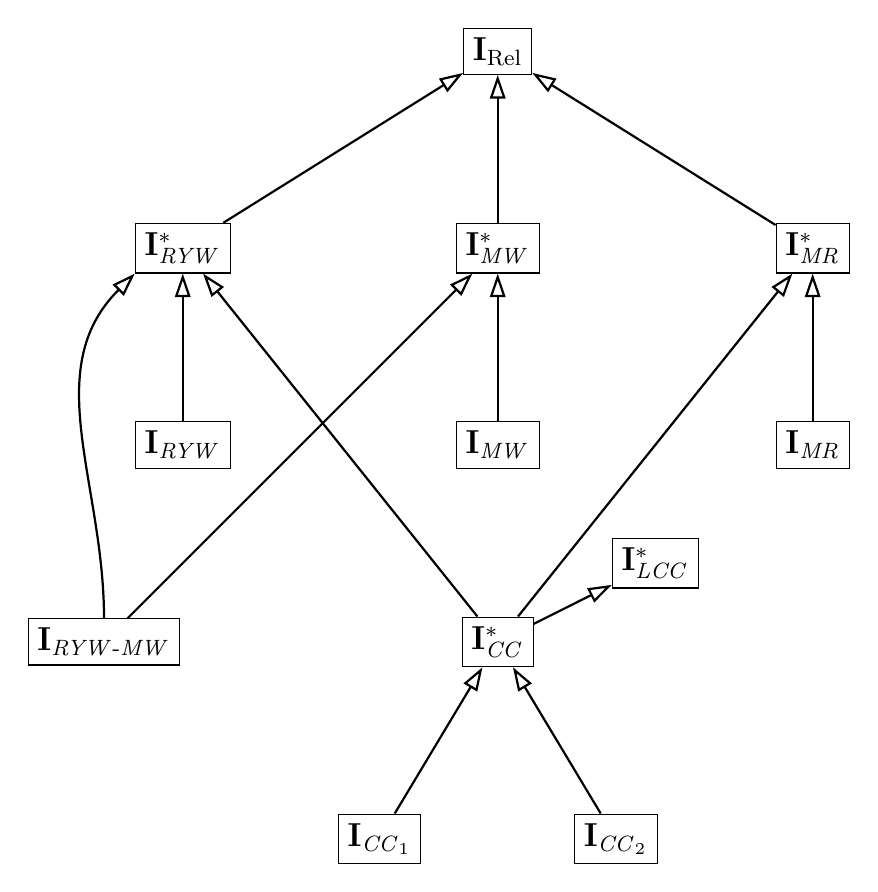
\begin{tikzpicture}[
    every node/.style={font=\large},
    arr/.style={-{Triangle[open, length=3mm]}, thick},
  ]

  % ── Nodes ────────────────────────────────────────────────────────────────

  % Bottom level
  \node[draw] (CC1)    at (-1.5, 0)  {$\mathbf{I}_{\CC_1}$};
  \node[draw] (CC2)    at ( 1.5, 0)  {$\mathbf{I}_{\CC_2}$};

  % Level 1
  \node[draw] (RYWMW)  at (-5,  2.5) {$\mathbf{I}_{\RYW\text{-}\MW}$};
  \node[draw] (CCstar) at ( 0,  2.5) {$\mathbf{I}_{\CC}^{*}$};

  % Level 2 (non-starred)
  \node[draw] (RYW)    at (-4, 5)    {$\mathbf{I}_{\RYW}$};
  \node[draw] (MW)     at ( 0, 5)    {$\mathbf{I}_{\MW}$};
  \node[draw] (MR)     at ( 4, 5)    {$\mathbf{I}_{\MR}$};
  \node[draw] (LCCstar) at ( 2, 3.5)   {$\mathbf{I}_{\LCC}^{*}$};

  % Level 3 (starred)
  \node[draw] (RYWstar) at (-4, 7.5) {$\mathbf{I}_{\RYW}^{*}$};
  \node[draw] (MWstar)  at ( 0, 7.5) {$\mathbf{I}_{\MW}^{*}$};
  \node[draw] (MRstar)  at ( 4, 7.5) {$\mathbf{I}_{\MR}^{*}$};

  % Level 4 (top)
  \node[draw] (Rel)     at ( 0, 10)  {$\mathbf{I}_{\mathrm{Rel}}$};

  % ── Edges ────────────────────────────────────────────────────────────────

  % CC1, CC2 → CC*
  \draw[arr] (CC1)     -- (CCstar);
  \draw[arr] (CC2)     -- (CCstar);

  % RYW-MW → RYW* (routed left of RYW to avoid overlap)
  \draw[arr] (RYWMW.north) to[out=90, in=225] (RYWstar.south west);

  % RYW-MW → MW*
  \draw[arr] (RYWMW)   -- (MWstar);

  % CC* → RYW*, MR*, LCC*
  \draw[arr] (CCstar)  -- (RYWstar);
  \draw[arr] (CCstar)  -- (MRstar);
  \draw[arr] (CCstar)  -- (LCCstar);

  % RYW → RYW*,  MW → MW*,  MR → MR*
  \draw[arr] (RYW)     -- (RYWstar);
  \draw[arr] (MW)      -- (MWstar);
  \draw[arr] (MR)      -- (MRstar);

  % RYW*, MW*, MR* → Rel
  \draw[arr] (RYWstar) -- (Rel);
  \draw[arr] (MWstar)  -- (Rel);
  \draw[arr] (MRstar)  -- (Rel);

  \end{tikzpicture}

  \vspace{0.5em}
  {\small
  \begin{tabular}{@{}ll@{}}
    $\mathbf{I}_{\mathrm{Rel}}$        & Relaxed Specification (Fig.~\ref{fig:relaxed-specification}) \\
    $\mathbf{I}_{\RYW}^{*}$           & Read Your Writes Specification (Fig.~\ref{fig:read-your-writes-spec}) \\
    $\mathbf{I}_{\RYW}$               & Read Your Writes Implementation (Fig.~\ref{fig:read-your-writes-impl}) \\
    $\mathbf{I}_{\MR}^{*}$            & Monotonic Reads Specification (Fig.~\ref{fig:monotonic-reads-spec}) \\
    $\mathbf{I}_{\MR}$                & Monotonic Reads Implementation (Fig.~\ref{fig:monotonic-reads-impl}) \\
    $\mathbf{I}_{\MW}^{*}$            & Monotonic Writes Specification (Fig.~\ref{fig:monotonic-writes-spec}) \\
    $\mathbf{I}_{\MW}$                & Monotonic Writes Implementation (Fig.~\ref{fig:monotonic-writes-impl}) \\
    $\mathbf{I}_{\RYW\text{-}\MW}$    & Read Your Writes and Monotonic Writes Implementation (Fig.~\ref{fig:ryw-mw-impl}) \\
    $\mathbf{I}_{\LCC}^{*}$           & Labeled Causal Consistency Spec (Fig.~\ref{fig:lcc-spec}) \\
    $\mathbf{I}_{\CC}^{*}$            & Causal Consistency Spec (Fig.~\ref{fig:causal-cons-spec}) \\
    $\mathbf{I}_{\CC_1}$              & Causal Consistency Implementation 1 (Fig.~\ref{fig:causal-map-95}) \\
    $\mathbf{I}_{\CC_2}$              & Causal Consistency Implementation 2 (Fig.~\ref{fig:LloydFreedman-protocol}) \\
  \end{tabular}
  }

  \caption{Refinement Hierarchy}
  \label{fig:refinement-hierarchy}
\end{figure}


\clearpage
\begin{figure}
\centering
\specfig{%
\begin{minipage}{0.90\linewidth}
   \figurealgtextsize
   \setlength{\abovedisplayskip}{0pt}%
   \setlength{\abovedisplayshortskip}{0pt}%
   \setlength{\belowdisplayskip}{0pt}%
   \setlength{\belowdisplayshortskip}{0pt}%
   \begin{mathpar}
   \begin{array}{|lr|}
      \hline
         𝐈_{\Rel} \ (\name{Relaxed Specification})
      & \\ \hline
         \CState ≔ \Unit
         & \bnote{Client State}
      \\
         \cInit(c) ≔ ⊥
         & \bnote{Client Initial State}
      \\
         \RState ≔ K ↦ V
         & \bnote{Replica State}
      \\
         \rInit(r, v₀) ≔ [\overline{ k ↦ v₀}]
         & \bnote{Replica Initial State}
      \\
      & \\
         \GetReqPayload ≔ \GetResPayload ≔ \Unit
         & \note{Get payload types}
      \\
         \getReq \ (\_) (\_, σ)  ≔ 
         & \note{At client: } \bnote{Get Request}
      \\ \t
         \ret〈○, p〉
         & \note{No payload}
      \\
         \getGuard \ (\_) (\_) (\_, \_, \_) ≔
         & \note{At replica: } \bnote{Get Guard}
      \\ \t
         \ret \true
         & \note{}
      \\
         \get \ (k) (\_) (\_, \_, ς)  ≔
         & \note{At replica: } \bnote{Get}
      \\ \t
         \llet〈v, \_〉← ς (k)
         & \note{}
      \\ \t
         \ret〈 v, ○, ς 〉
         & \note{No payload}
      \\
         \getRes \ (\_, \_) (\_) (\_, σ) ≔
         & \note{At client: } \bnote{Get Response}
      \\ \t
         \ret σ
         & \note{}
      \\
      & \\
         \PutReqPayload ≔ \Unit
         & \note{Put payload types} 
      \\
         \putReq \ (k, \_) (\_, σ) ≔ 
         & \note{At client: }\bnote{Put Request}
      \\ \t
         \ret〈○, σ〉
         & \note{No payload}
      \\
         \putGuard \ (\_, \_) (\_) (\_, \_, \_) ≔ 
         & \note{At replica: } \bnote{Put Guard}
      \\ \t
         \ret \true
         & \note{}          
      \\
         \lput \ (k, v) (\_) (\_, \_, ς) ≔ 
         & \note{At replica: } \bnote{Put}
      \\ \t
         \ret ς [k ↦ v]
      & \\ \hline
   \end{array}
   \end{mathpar}
\end{minipage}%
}
   \caption{Relaxed Specification}
   \label{fig:relaxed-specification}
\end{figure}


\subsection{Read-Your-Writes (RYW)}
A client's read sees its own most recent write. The session tracks every put the client has issued; the get-guard requires the responding replica to have applied every put in that set (\cref{fig:read-your-writes-spec}). The reference implementation stores per-replica state as a function from key to timestamp (\cref{fig:read-your-writes-impl}).


\clearpage
\begin{figure}
   \figurealgtextsize
   \setlength{\abovedisplayskip}{0pt}%
   \setlength{\abovedisplayshortskip}{0pt}%
   \setlength{\belowdisplayskip}{0pt}%
   \setlength{\belowdisplayshortskip}{0pt}%
   \begin{mathpar}
   \begin{array}{|lr|}
      \hline
         𝐈_{\RYW} ⃰  \ (\name{Read Your Writes Specification}) 
      & \\ \hline
         T ≔ \Nat
         & \note{Timestamp}
      \\
         \CState ≔ 
         & \bnote{Client State}
      \\ \t
%          \Set[C × T × K]
%          & \note{Session puts. ($C × T$ uniquely identifies puts.)}
         \Set[K × T]
         & \note{Session puts. ($T$ uniquely identifies puts in a client.)}
      \\
         \cInit(c) ≔
         & \bnote{Client Initial State}
      \\ \t
         ∅
%          \lif (c = c₀) \
%            \{ 〈c₀, 1〉\} \ 
%          \lelse ∅
         & \note{No initial puts}
      \\
         \RState ≔
         & \bnote{Replica State}
      \\ \t
%          K ↦ (C × T × V × \Set[C × T × K])
         K ↦ (V × C × T \, × 
         & \note{Map from each key $k$ to its value $v$, its origin $〈c, t〉$,}
      \\ \t \phantom{K ↦ (}
%          \Set[C × T])
         \Set[T])
         & \note{and timestamps of puts on $k$ before it.}
      \\
         \rInit(r, v₀) ≔ 
         & \bnote{Replica Initial State}
      \\ \t
         [\overline{ k ↦ 〈v₀, c₀, 0, ∅〉}]
%          [\overline{ k ↦ 〈v₀, c₀, 1, ∅〉}]
         & \note{}
      \\
      & \\
%          \GetReqPayload ≔ \Set[C × T × K]
%          \GetReqPayload ≔ \Set[C × T]
         \GetReqPayload ≔ \Set[T]
         & \note{Get payload types}
      \\
         \GetResPayload ≔ \Unit
      & \\
         \getReq \ (k) (\_, p)  ≔ 
         & \note{At client: } \bnote{Get Request}
      \\ \t
         \ret〈p|ₖ, p〉
         & \note{Session past puts as request payload, State unchanged}
      \\
         \getGuard \ (k)(p)(c, \_, ς) ≔
         & \note{At replica: } \bnote{Get Guard}
      \\ \t
         \llet〈\_, c', t', p'〉← ς (k)
      & \\ \t
%          \ret c = c' ⇒ ¬ (p'|ₖ ∪ \{〈c', t'〉\} ⊂ p|ₖ )
%          \ret c' = c ⇒ ¬ (p' ∪ \{〈c', t'〉\} ⊂ p )
%          \ret c = c' ⇒ p = p' ∪ \{〈c', t'〉\}
%          \ret c = c' ⇒ p ⊆ p' ∪ \{〈c', t'〉\}
         \ret c = c' ⇒ p ⊆ p' ∪ \{ t'\}
%          \ret p|ₖ ⊆ (p'|ₖ ∪ \{〈c', t', k〉\})         
         & \note{If stored value is from requesting client, his puts not missed.}
%          
%       & \\ \t
%          \ret 
%             \lforall (λ〈c ⃰, t ⃰, k ⃰〉. \
%             & \note{If the session puts $d$}
%       \\ \t\t \phantom{\ret \lforall (}
%             k ⃰ = k  ⇒ 
%             & \note{includes any put $〈c ⃰, t ⃰〉$,}
%       \\ \t\t\t \phantom{\ret \lforall (}
%             t ⃰ = 0 ∨〈c ⃰, t ⃰〉= 〈c', t'〉\ ∨
%             & \note{then the current entry for $k$ is $〈c ⃰, t ⃰〉$, or}
%       \\ \t\t\t \phantom{\ret \lforall (}
%             〈c ⃰, t ⃰, k ⃰〉∈ p') \
%             & \note{$〈c ⃰, t ⃰〉$ is in the past puts of the current entry.}
%       \\ \t \phantom{\ret \lforall}
%             p
%          & \note{}
      \\
         \get \ (k) (\_) (\_, \_, ς)  ≔
         & \note{At replica: } \bnote{Get}
      \\ \t
         \llet〈v, \_, \_, \_〉← ς (k)
         & \note{}
      \\ \t
         \ret〈 v, ○, ς 〉
         & \note{No payload}
      \\
         \getRes \ (\_, \_) (\_) (\_, p) ≔
         & \note{At client: } \bnote{Get Response}
      \\ \t
         \ret p
         & \note{State unchanged.}
      \\
      & \\
%          \PutReqPayload ≔ T × \Set[C × T]
         \PutReqPayload ≔ T × \Set[T]
         & \note{Put payload types}
      \\
         \putReq \ (k, \_) (\self, p) ≔ 
         & \note{At client: }\bnote{Put Request}
      \\ \t
         \llet t ← |p| + 1
         & \note{Current put timestamp}
      \\ \t
%          \llet p' ← p ∪ \{〈\self, t, k〉\}
         \llet p' ← p ∪ \{〈t, k〉\}
         & \note{The put is added to session puts.}
      \\ \t
%          \ret〈d|ₖ, d'〉
         \ret〈〈t, p|ₖ〉, p'〉
         & \note{Session puts are sent as request payload.}
      \\
         \putGuard \ (\_, \_) (\_) (\_, \_, \_) ≔ 
         & \note{At replica: } \bnote{Put Guard}
      \\ \t
         \ret \true
         & \note{}          
      \\
         \lput \ (k, v) (〈t, p〉) (c, \_, ς) ≔ 
         & \note{At replica: } \bnote{Put}
      \\ \t
         \ret ς [k ↦ 〈v, c, t, p〉]
      & \\
      & \\
      p|ₖ ≔ \{ t \ | \ 〈t, k〉∈ p \}
      & \\ \hline
   \end{array}
   \end{mathpar}
   \caption{Read Your Writes Specification}
   \label{fig:read-your-writes-spec}
\end{figure}


\clearpage
\begin{figure}
   \figurealgtextsize
   \setlength{\abovedisplayskip}{0pt}%
   \setlength{\abovedisplayshortskip}{0pt}%
   \setlength{\belowdisplayskip}{0pt}%
   \setlength{\belowdisplayshortskip}{0pt}%
   \begin{mathpar}
   \begin{array}{|lr|}
      \hline
         𝐈_{\RYW} \ (\name{Read Your Writes Implementation}) 
      & \\ \hline
         T ≔ \Nat
         & \note{Timestamp}
      \\
         \CState ≔ 
         & \bnote{Client State}
      \\ \t
         K ↦ T
         & \note{Latest put for each key. ($T$ uniquely identifies puts in a client.)}
      \\
         \cInit(c) ≔
         & \bnote{Client Initial State}
      \\ \t
         [ \overline{k ↦ 0} ]
         & \note{No initial puts}
      \\
         \RState ≔
         & \bnote{Replica State}
      \\ \t
         K ↦ (V × C × T) 
         & \note{Map from each key $k$ to its value $v$, and its origin $〈c, t〉$}
      \\
         \rInit(r, v₀) ≔ 
         & \bnote{Replica Initial State}
      \\ \t
         [\overline{ k ↦ 〈v₀, c₀, 0〉}]
         & \note{}
      \\
      & \\
         \GetReqPayload ≔ T
         & \note{Get payload types}
      \\
         \GetResPayload ≔ \Unit
      & \\
         \getReq \ (k) (\_, p)  ≔ 
         & \note{At client: } \bnote{Get Request}
      \\ \t
         \ret〈p(k), p〉
         & \note{Timestamp of latest put as request payload, State unchanged}
      \\
         \getGuard \ (k)(t)(c, \_, ς) ≔
         & \note{At replica: } \bnote{Get Guard}
      \\ \t
         \llet〈\_, c', t'〉← ς (k)
      & \\ \t
         \ret  c = c'  ⇒  t = t' 
%          t ≤ t'
         & \note{If stored value is from requesting client, his puts not missed.}
      \\
         \get \ (k) (\_) (\_, \_, ς)  ≔
         & \note{At replica: } \bnote{Get}
      \\ \t
         \llet〈v, \_, \_〉← ς (k)
         & \note{}
      \\ \t
         \ret〈 v, ○, ς 〉
         & \note{No payload}
      \\
         \getRes \ (\_, \_) (\_) (\_, p) ≔
         & \note{At client: } \bnote{Get Response}
      \\ \t
         \ret p
         & \note{State unchanged.}
      \\
      & \\
         \PutReqPayload ≔ T
         & \note{Put payload types}
      \\
         \putReq \ (k, \_) (\self, p) ≔ 
         & \note{At client: }\bnote{Put Request}
      \\ \t
         \llet t ← p(k) + 1
         & \note{Current put timestamp}
      \\ \t
         \llet p' ← p [ k ↦ t ]
         & \note{The put timestamp is stored as the latest for the key.}
      \\ \t
         \ret〈t, p'〉
         & \note{Latest put timestamp sent as request payload.}
      \\
         \putGuard \ (\_, \_) (\_) (\_, \_, \_) ≔ 
         & \note{At replica: } \bnote{Put Guard}
      \\ \t
         \ret \true
         & \note{}          
      \\
         \lput \ (k, v) (t) (c, \_, ς) ≔
         & \note{At replica: } \bnote{Put}
      \\ \t
         \ret ς [k ↦ 〈v, c, t〉]
      & \\ \hline
   \end{array}
   \end{mathpar}
   \caption{Read Your Writes Implementation}
   \label{fig:read-your-writes-impl}
\end{figure}


\subsection{Monotonic Reads (MR)}
A client's reads respect the order of writes the client has previously observed. The session keeps the set of writes seen so far; subsequent reads must return values applied no earlier than every write in that set (\cref{fig:monotonic-reads-spec}). The reference implementation stores per-replica state as a function from key to (value, client, timestamp); the get-guard checks every entry against the client's session set on every read (\cref{fig:monotonic-reads-impl}).

\clearpage
\begin{figure}
   \figurealgtextsize
   \setlength{\abovedisplayskip}{0pt}%
   \setlength{\abovedisplayshortskip}{0pt}%
   \setlength{\belowdisplayskip}{0pt}%
   \setlength{\belowdisplayshortskip}{0pt}%
   \begin{mathpar}
   \begin{array}{|lr|}
      \hline
         𝐈_{\MR} ⃰  \ (\name{Monotonic Reads Specification})
      & \\ \hline
         T ≔ \Nat
         & \note{Timestamp}
      \\
         \CState ≔ 
         & \bnote{Client State}
      \\ \t
         \Set[T × K] \, ×
         & \note{Session puts. ($C × T$ uniquely identifies puts.)}
      \\ \t 
         \Set[C × T × K]
         & \note{Session dependencies.}         
      \\
         \cInit(c) ≔
         & \bnote{Client Initial State}
      \\ \t
         ∅
         & \note{No initial dependencies}
      \\
         \RState ≔
         & \bnote{Replica State}
      \\ \t
         K ↦ (V × C × T \, ×
         & \note{Map from each key $K$ to its value $V$, its origin $C × T$}
      \\ \t \phantom{K ↦ (}
%          \Set[C × T])
         \Set[T  × K])
         & \note{and puts before it}
      \\
         \rInit(r, v₀) ≔ 
         & \bnote{Replica Initial State}
      \\ \t
         [\overline{ k ↦ 〈v₀, c₀, 0, ∅〉}]
         & \note{}
      \\
      & \\
%          \GetReqPayload ≔ \Set[C × T × K]
%          \GetReqPayload, \GetResPayload ≔ \Set[C × T]
%          \GetReqPayload, \GetResPayload ≔ \Set[C × T]
         \GetReqPayload ≔ \Set[C × T]
         & \note{Get payload types}
      \\
         \GetResPayload ≔ C × T
         & \note{}
      \\
         \getReq \ (k) (\_, 〈p, d〉)  ≔ 
         & \note{At client: } \bnote{Get Request}
      \\ \t
         \ret〈d|ₖ, 〈p, d〉〉
         & \note{Session deps for $k$ sent as payload, State unchanged}
      \\
         \getGuard \ (k) (d) (c, \_, ς) ≔
         & \note{At replica: } \bnote{Get Guard}
      \\ \t
         \llet〈\_, c', t', d'〉← ς (k)
      & \\ \t
%          \ret d|_{c'} ⊆ d' ∪ \{〈c', t'〉\}
         \ret d|_{c'} ⊆ d'|ₖ ∪ \{ t' \}
%          & \note{Observed puts from $c'$ are not after stored put from $c'$.}
         & \note{Stored put from $c'$ doesn't miss observed puts from $c'$.}
      \\
         \get \ (k) (\_) (\_, \_, ς)  ≔
         & \note{}
      \\ \t
         \llet〈v, c, t, d〉← ς (k)
      & \\ \t
         \ret〈 v, 〈c, t〉, ς 〉
         & \note{The stored put returned as a dependency.}
      \\
         \getRes \ (k, \_) (〈c, t〉) (\_, 〈p, d〉) ≔
         & \note{At client: } \bnote{Get Response}
      \\ \t
%          \ret d ∪ (c ▹ d' ▹ k)
         \ret 〈p, d ∪ \{ 〈c, t, k〉\}〉
%          \ret d ∪ d'
%          \ret d ∪ (c ▹ d')
%          \ret d ∪ (\lmap (λ〈t, k〉. \ 〈c, t, k〉) \ d'
         & \note{Returned dependency added to session dependencies.}
      \\
      & \\
         \PutReqPayload ≔ T × \Set[T × K]
         & \note{Put payload types}
      \\
         \putReq \ (k, \_) (\_, 〈p, d〉) ≔ 
         & \note{At client: }\bnote{Put Request}
      \\ \t
%          \llet t ← |\{〈c, \_, \_〉∈ p \ | \ c=\self \}| + 1
%          \llet t ← | \, d|_\self \, | + 1
         \llet t ← | p | + 1
         & \note{Current put timestamp}
      \\ \t
         \llet p' ← p ∪ \{〈t, k〉\}
         & \note{The put is added to session puts.}
      \\ \t
%          \ret〈〈t, d|ₖ|ₚ〉, d'〉
%          \ret〈〈t, d|_{\self}|ₖ〉, d'〉
         \ret〈〈t, p〉, 〈p', d〉〉
         & \note{Session puts are sent as request payload.}
      \\
         \putGuard \ (\_, \_) (\_) (\_, \_, \_) ≔ 
         & \note{At replica: } \bnote{Put Guard}
      \\ \t
         \ret \true
         & \note{}          
      \\
         \lput \ (k, v) (〈t, p〉) (c, \_, ς) ≔ 
         & \note{At replica: } \bnote{Put}
      \\ \t
         \ret ς [k ↦ 〈v, c, t, p〉]
      & \\
      & \\
      d|ₖ ≔ \{〈c, t〉 \ | \ 〈c, t, k〉∈ d \}
      & \\
      d|ₖ ≔ \{ t \ | \ 〈t, k〉∈ d \}
%       & \\
%       d|_c  ≔ \{〈t, k〉 \ | \ 〈c, t, k〉∈ d \}
      & \\
      d|_c  ≔ \{ t \ | \ 〈c, t〉∈ d \}
%       & \\
%       c ▹ d ≔ \lmap (λ〈t, k〉. \ 〈c, t, k〉) \ d
      & \\ \hline
   \end{array}
   \end{mathpar}
   \caption{Monotonic Reads Specification}
   \label{fig:monotonic-reads-spec}
\end{figure}

\clearpage
\begin{figure}
   \figurealgtextsize
   \setlength{\abovedisplayskip}{0pt}%
   \setlength{\abovedisplayshortskip}{0pt}%
   \setlength{\belowdisplayskip}{0pt}%
   \setlength{\belowdisplayshortskip}{0pt}%
   \begin{mathpar}
   \begin{array}{|lr|}
      \hline
         𝐈_{\MR} \ (\name{Monotonic Reads Implementation})
      & \\ \hline
         T ≔ \Nat
         & \note{Timestamp}
      \\
         \CState ≔ 
         & \bnote{Client State}
      \\ \t
         T \ ×
         & \note{Session latest put timestamp}
      \\ \t
         K ↦ C ↦ T
         & \note{Largest timestamp read for the key from the client.}         
      \\
         \cInit(c) ≔
         & \bnote{Client Initial State}
      \\ \t
         〈∅, ∅〉
         & \note{No initial puts and dependencies}
      \\
         \RState ≔
         & \bnote{Replica State}
      \\ \t
         K ↦ (V × C × T)
         & \note{Map from each key $K$ to its value $V$, its origin $C × T$}
%       \\ \t \phantom{K ↦ (}
% %          \Set[C × T])
%          K ↦ T)
%          & \note{and puts before it}
      \\
         \rInit(r, v₀) ≔ 
         & \bnote{Replica Initial State}
      \\ \t
         [\overline{ k ↦ 〈v₀, c₀, 0〉}]
         & \note{}
      \\
      & \\
         \GetReqPayload ≔ \Set[C × T]
         & \note{Get payload types}
      \\
         \GetResPayload ≔ C × T
         & \note{}
      \\
         \getReq \ (k) (\_, 〈t, d〉)  ≔ 
         & \note{At client: } \bnote{Get Request}
      \\ \t
         \ret〈d(k), 〈t, d〉〉
         & \note{Session deps for $k$ sent as payload, State unchanged}
      \\
         \getGuard \ (k) (d) (c, \_, ς) ≔
         & \note{At replica: } \bnote{Get Guard}
      \\ \t
         \llet〈\_, c', t'〉← ς (k)
      & \\ \t
         \ret d(c') ≤  t'
         & \note{Stored put from $c'$ doesn't miss observed puts from $c'$.}
      \\
         \get \ (k) (\_) (\_, \_, ς)  ≔
         & \note{}
      \\ \t
         \llet〈v, c, t〉← ς (k)
      & \\ \t
         \ret〈 v, 〈c, t〉, ς 〉
         & \note{The stored put returned as a dependency.}
      \\
         \getRes \ (k, \_) (〈c, t〉) (\_, 〈t, d〉) ≔
         & \note{At client: } \bnote{Get Response}
      \\ \t
         \ret〈t, d[〈k,c〉 ↦ t] 〉
         & \note{Returned dependency advances session dependencies.}
      \\
      & \\
         \PutReqPayload ≔ T
         & \note{Put payload types}
      \\
         \putReq \ (k, \_) (\_, 〈t, d〉) ≔ 
         & \note{At client: }\bnote{Put Request}
      \\ \t
         \llet t' ← t + 1
         & \note{Current put timestamp}
      \\ \t
         \ret〈t', 〈t', d〉〉
         & \note{}
      \\
         \putGuard \ (\_, \_) (\_) (\_, \_, \_) ≔ 
         & \note{At replica: } \bnote{Put Guard}
      \\ \t
         \ret \true
         & \note{}          
      \\
         \lput \ (k, v) (t) (c, \_, ς) ≔ 
         & \note{At replica: } \bnote{Put}
      \\ \t
         \ret ς [k ↦ 〈v, c, t〉]
      & \\ \hline
   \end{array}
   \end{mathpar}
   \caption{Monotonic Reads Implementation}
   \label{fig:monotonic-reads-impl}
\end{figure}


\subsection{Monotonic Writes (MW)}
A single client's writes are observed in order at every replica that observes them. Each replica records, per writing client, the latest applied timestamp; the put-guard rejects any out-of-order delivery (\cref{fig:monotonic-writes-spec}). The reference implementation prepends the timestamp of each new write to a per-key list with no de-duplication, so receivers can re-check ordering on every delivery (\cref{fig:monotonic-writes-impl}).


\clearpage
\begin{figure}
   \figurealgtextsize
   \setlength{\abovedisplayskip}{0pt}%
   \setlength{\abovedisplayshortskip}{0pt}%
   \setlength{\belowdisplayskip}{0pt}%
   \setlength{\belowdisplayshortskip}{0pt}%
   \begin{mathpar}
   \begin{array}{|lr|}
      \hline
         𝐈_{\MW} ⃰  \ (\name{Monotonic Writes Specification}) 
      & \\ \hline
         T ≔ \Nat
         & \note{Timestamp}
      \\
         \CState ≔ 
         & \bnote{Client State}
      \\ \t
         \Set[T × K]
         & \note{Session puts. ($C × T$ uniquely identifies puts.)}
      \\
         \cInit(c) ≔
         & \bnote{Client Initial State}
      \\ \t
         ∅
         & \note{No initial dependencies}
      \\
         \RState ≔
         & \bnote{Replica State}
      \\ \t
         K ↦ (V × \Set[C × T])
         & \note{Map from each key $K$ to its value $V$, and puts already applied.}
      \\
         \rInit(r, v₀) ≔ 
         & \bnote{Replica Initial State}
      \\ \t
         [\overline{ k ↦ 〈v₀, ∅〉}]
         & \note{}
      \\
      & \\
         \GetReqPayload ≔ \GetResPayload ≔ \Unit
         & \note{Get payload types}
      \\
         \getReq \ (\_) (\_, p)  ≔ 
         & \note{At client: } \bnote{Get Request}
      \\ \t
         \ret〈○, p〉
         & \note{Session past puts as request payload, State unchanged}
      \\
         \getGuard \ (\_) (\_) (\_, \_, \_) ≔
         & \note{At replica: } \bnote{Get Guard}
      \\ \t
         \ret \true
         & \note{}
      \\
         \get \ (k) (\_) (\_, \_, ς)  ≔
         & \note{At replica: } \bnote{Get}
      \\ \t
         \llet〈v, \_〉← ς (k)
         & \note{}
      \\ \t
         \ret〈 v, ○, ς 〉
         & \note{No payload}
      \\
         \getRes \ (\_, \_) (\_) (\_, p) ≔
         & \note{At client: } \bnote{Get Response}
      \\ \t
         \ret p
         & \note{State unchanged.}
      \\
      & \\
         \PutReqPayload ≔ T × \Set[T]
         & \note{Put payload types}
      \\
         \putReq \ (k, \_) (\_, p) ≔ 
         & \note{At client: }\bnote{Put Request}
      \\ \t
         \llet t ← |p| + 1
         & \note{Current put timestamp}
      \\ \t
         \llet p' ← p ∪ \{〈t, k〉\}         
         & \note{The put is added to session puts.}
      \\ \t
         \ret〈〈t, p|ₖ〉, p'〉
         & \note{Session puts for the key are sent as request payload.}
      \\
         \putGuard \ (k, \_) (〈t, p〉) (c, \_, ς) ≔ 
         & \note{At replica: } \bnote{Put Guard}
      \\ \t
         \llet〈\_, p'〉← ς (k)
      & \\ \t
         \ret p ⊆ p'|_c
         & \note{Previous puts of session already applied.}
      \\
         \lput \ (k, v) (〈t, \_〉) (c, \_, ς) ≔ 
         & \note{At replica: } \bnote{Put}
      \\ \t
         \llet〈\_, p'〉← ς (k)
         & \note{}
      \\ \t
         \ret ς [k ↦ 〈v, p' ∪ \{〈c,t〉\}]
      & \\
      & \\
      p|ₖ ≔ \{ t \ | \ 〈t, k〉∈ p \}
      & \\
      p|_c  ≔ \{ t \ | \ 〈c, t〉∈ p \}
      & \\ \hline
   \end{array}
   \end{mathpar}
   \caption{Monotonic Writes Specification}
   \label{fig:monotonic-writes-spec}
\end{figure}


\clearpage
\begin{figure}
   \figurealgtextsize
   \setlength{\abovedisplayskip}{0pt}%
   \setlength{\abovedisplayshortskip}{0pt}%
   \setlength{\belowdisplayskip}{0pt}%
   \setlength{\belowdisplayshortskip}{0pt}%
   \begin{mathpar}
   \begin{array}{|lr|}
      \hline
         𝐈_{\MW} \ (\name{Monotonic Writes Implementation}) 
      & \\ \hline
         T ≔ \Nat
         & \note{Timestamp}
      \\
         \CState ≔ 
         & \bnote{Client State}
%       \\ \t
%          T \ ×
%          & \note{Latest timestamp, and}
      \\ \t         
         K ↦ T
         & \note{Latest timestamp of puts for the key.}
      \\
         \cInit(c) ≔
         & \bnote{Client Initial State}
      \\ \t
%          〈0, \overline{k ↦ 0}〉
         \overline{k ↦ 0}
         & \note{No initial puts}
      \\
         \RState ≔
         & \bnote{Replica State}
      \\ \t
         K ↦ (V \ ×
         & \note{Map from each key $K$ to its value $V$, and}
      \\ \t \phantom{K ↦ (}
         C ↦ T)
         & \note{latest puts applied from sessions.}
      \\
         \rInit(r, v₀) ≔ 
         & \bnote{Replica Initial State}
      \\ \t
         [\overline{ k ↦ 〈v₀, \overline{c ↦ 0}〉}]
         & \note{}
      \\
      & \\
         \GetReqPayload ≔ \GetResPayload ≔ \Unit
         & \note{Get payload types}
      \\
         \getReq \ (\_) (\_, σ)  ≔ 
         & \note{At client: } \bnote{Get Request}
      \\ \t
         \ret〈○, σ〉
         & \note{Session past puts as request payload, State unchanged}
      \\
         \getGuard \ (\_) (\_) (\_, \_, \_) ≔
         & \note{At replica: } \bnote{Get Guard}
      \\ \t
         \ret \true
         & \note{}
      \\
         \get \ (k) (\_) (\_, \_, ς)  ≔
         & \note{At replica: } \bnote{Get}
      \\ \t
         \llet〈v, \_〉← ς (k)
         & \note{}
      \\ \t
         \ret〈 v, ○, ς 〉
         & \note{No payload}
      \\
         \getRes \ (\_, \_) (\_) (\_, σ) ≔
         & \note{At client: } \bnote{Get Response}
      \\ \t
         \ret σ
         & \note{State unchanged.}
      \\
      & \\
         \PutReqPayload ≔ T
         & \note{Put payload types}
      \\
         \putReq \ (k, \_) (\_, p) ≔ 
         & \note{At client: }\bnote{Put Request}
      \\ \t
         t ← p(k)
         & \note{}
      \\ \t
         \llet p' ← p [ k ↦ t + 1]
         & \note{The timestamp of the latest put for key is advanced.}
      \\ \t
         \ret〈t, p'〉
         & \note{Latest put timestamp for the key is sent as request payload.}
      \\
         \putGuard \ (k, \_) (t) (c, \_, ς) ≔ 
         & \note{At replica: } \bnote{Put Guard}
      \\ \t
         \llet〈\_, p'〉← ς (k)
      & \\ \t
         \ret  p'(c) = t
         & \note{Previous puts of session already applied.}
      \\
         \lput \ (k, v) (t) (c, \_, ς) ≔ 
         & \note{At replica: } \bnote{Put}
      \\ \t
         \llet〈\_, p'〉← ς (k)
         & \note{}
      \\ \t
         \ret ς [k ↦ 〈v, p' [c ↦ t + 1]〉]
         & \note{}
      \\ \hline
   \end{array}
   \end{mathpar}
   \caption{Monotonic Writes Implementation}
   \label{fig:monotonic-writes-impl}
\end{figure}


\subsection{Read-Your-Writes $+$ Monotonic Writes (RYW+MW)}
Composition of Read-Your-Writes and Monotonic Writes. RYW+MW is the conjunction of RYW and MW rather than an independent property; an implementation satisfies it iff it refines both, so correctness is the joint refinement obligation. The reference combines RYW's read-side check with MW's compare-and-swap on every put (\cref{fig:ryw-mw-impl}).

\clearpage
\begin{figure}
   \figurealgtextsize
   \setlength{\abovedisplayskip}{0pt}%
   \setlength{\abovedisplayshortskip}{0pt}%
   \setlength{\belowdisplayskip}{0pt}%
   \setlength{\belowdisplayshortskip}{0pt}%
   \begin{mathpar}
   \begin{array}{|lr|}
      \hline
         \multicolumn{2}{|l|}{𝐈_{\RYW\text{-}\MW} \ (\name{Read Your Writes and Monotonic Writes Implementation}) }         
      \\ \hline
         T ≔ \Nat
         & \note{Timestamp}
      \\
         \CState ≔ 
         & \bnote{Client State}
      \\ \t         
         K ↦ T
         & \note{Latest timestamp of puts for the key.}
      \\
         \cInit(c) ≔
         & \bnote{Client Initial State}
      \\ \t
         \overline{k ↦ 0}
         & \note{No initial puts}
      \\
         \RState ≔
         & \bnote{Replica State}
      \\ \t
         K ↦ (V × C \ × 
         & \note{Map from each key $K$ to its value $V$, and its originating sessions $C$,}
      \\ \t \phantom{K ↦ (}
         C ↦ T)
         & \note{latest puts applied from sessions}
      \\
         \rInit(r, v₀) ≔ 
         & \bnote{Replica Initial State}
      \\ \t
         [\overline{ k ↦ 〈v₀, 0, \overline{c ↦ 0}〉}]
         & \note{}
      \\
      & \\
         \GetReqPayload ≔ T
         & \note{Get payload types}
      \\
         \GetResPayload ≔ \Unit
      & \\
         \getReq \ (k) (\_, p)  ≔ 
         & \note{At client: } \bnote{Get Request}
      \\ \t
         \ret〈p(k), p〉
         & \note{Timestamp of latest put as request payload, State unchanged}
      \\
         \getGuard \ (k)(t)(c, \_, ς) ≔
         & \note{At replica: } \bnote{Get Guard}
      \\ \t
         \llet〈\_, c', p'〉← ς (k)
      & \\ \t
         \ret  c = c'  ⇒  p'(c') = t
%          t ≤ t'
         & \note{If stored value is from requesting client, his puts not missed.}
      \\
         \get \ (k) (\_) (\_, \_, ς)  ≔
         & \note{At replica: } \bnote{Get}
      \\ \t
         \llet〈v, \_, \_〉← ς (k)
         & \note{}
      \\ \t
         \ret〈 v, ○, ς 〉
         & \note{No payload}
      \\
         \getRes \ (\_, \_) (\_) (\_, p) ≔
         & \note{At client: } \bnote{Get Response}
      \\ \t
         \ret p
         & \note{State unchanged.}
      \\
      & \\
         \PutReqPayload ≔ T
         & \note{Put payload types}
      \\
         \putReq \ (k, \_) (\_, p) ≔ 
         & \note{At client: }\bnote{Put Request}
      \\ \t
         t ← p(k)
         & \note{}
      \\ \t
         \llet p' ← p [ k ↦ t + 1 ]
         & \note{The timestamp of the latest put for key is advanced.}
      \\ \t
         \ret〈t, p'〉
         & \note{Latest put timestamp for the key is sent as request payload.}
      \\
         \putGuard \ (k, \_) (t) (c, \_, ς) ≔ 
         & \note{At replica: } \bnote{Put Guard}
      \\ \t
         \llet〈\_, \_, p'〉← ς (k)
      & \\ \t
         \ret p'(c) = t
         & \note{Previous puts of session already applied.}
      \\
         \lput \ (k, v) (t) (c, \_, ς) ≔ 
         & \note{At replica: } \bnote{Put}
      \\ \t
         \llet〈\_, p'〉← ς (k)
         & \note{}
      \\ \t
         \ret ς [k ↦ 〈v, c, p' [c ↦ t + 1]〉]
         & \note{}
      \\ \hline
   \end{array}
   \end{mathpar}
   \caption{Read Your Writes and Monotonic Writes Implementation}
   \label{fig:ryw-mw-impl}
\end{figure}


\subsection{Causal Consistency (CC) and Labeled Causal Consistency (LCC)}
\textbf{Causal Consistency (CC).}
Cross-client causal consistency: every read returns a value whose causal predecessors have all been observed at the responding replica. Dependencies are tracked as explicit sets in the spec state (\cref{fig:causal-cons-spec}), which the implementation must bridge to its concrete representation (typically a per-client vector clock plus a compare-and-swap on the writer's own slot during put). Two reference implementations are given: a per-client vector-clock store (\cref{fig:causal-map-95}) and a Lloyd--Freedman-style protocol (\cref{fig:LloydFreedman-protocol}).

\noindent\textbf{Labeled Causal Consistency (LCC).}
Causal consistency parameterised by per-message topic labels and per-client interest masks. Every put is tagged with a label, and every client declares which labels it cares about; the get-guard requires the responding replica to have observed every dependency whose label is in the requesting client's mask (\cref{fig:lcc-spec}). To our knowledge this is the first \coq{} formalisation of LCC and the first verified implementation.



\clearpage
\begin{figure}
   \figurealgtextsize
   \setlength{\abovedisplayskip}{0pt}%
   \setlength{\abovedisplayshortskip}{0pt}%
   \setlength{\belowdisplayskip}{0pt}%
   \setlength{\belowdisplayshortskip}{0pt}%
   \begin{mathpar}
   \begin{array}{|lr|}
      \hline
         𝐈_{\CC} ⃰  \ (\name{Causal Consistency Spec}) 
      & \\ \hline
         T ≔ \Nat
         & \note{Timestamp}
      \\
         \CState ≔ 
         & \bnote{Client State}
      \\ \t
         〈\Set[C × T × K],
%          〈K ↦ \Set[C × T],
         & \note{Session dependencies from puts.}
      \\ \t \phantom{〈}
         \Set[\Set[C × T × K]] 〉
%          \Set[C × T]
%          & \note{Put timestamp, and Session dependencies}
%          & \note{Current timestamp, and Session dependencies.}
         & \note{Session dependencies from gets}
      \\ \t
         & \note{($C × T$ uniquely identifies puts.)}         
%       \\ \t
%          & \note{($C × T$ uniquely identifies puts.)}
      \\
         \cInit(c) ≔
         & \bnote{Client Initial State}
      \\ \t
%          〈0, ∅〉
         〈∅, ∅〉
%          \lif (c ≠ c₀) \
%          〈∅, ∅〉\ 
%          \lelse  〈[ \overline{k ↦〈c₀, k + 1〉}], ∅〉
         & \note{No initial dependencies}
      \\
         \RState ≔
         & \bnote{Replica State}
      \\ \t
         K ↦ (V × C × T \, × 
%          K ↦ (C × T × V × \Set [C × T])
         & \note{Map from each key $K$ to its value $V$, its origin $C × T$,}
      \\ \t \phantom{K ↦ (}         
         \Set[C × T × K])
         & \note{and set of dependencies}
      \\
         \rInit(r, v₀) ≔ 
         & \bnote{Replica Initial State}
      \\ \t
         [\overline{ k ↦ 〈v₀, c₀, 0, ∅〉}]
%          [\overline{ k ↦ 〈v₀, c₀, k+1, ∅〉}]
%          & \note{For each key, initial $v₀$ and empty initial dependencies}
         & \note{Empty initial dependencies}
      \\
      & \\
         \GetReqPayload ≔ 〈\Set[C × T × K],
         & \note{Get payload types}
      \\ \phantom{\GetReqPayload ≔ 〈}
         \Set[\Set[C × T × K]]\>
%          \GetReqPayload ≔ \Set[C × T]
         & \note{}
      \\
         \GetResPayload ≔ \Set[C × T  × K]
      & \\
         \getReq \ (k) (\_, 〈p, G〉)  ≔ 
         & \note{At client: } \bnote{Get Request}
      \\ \t
         \ret〈〈p|ₖ, G|ₖ〉, 〈p, G〉〉 
         & \note{Session deps sent as request payload, State unchanged}
      \\
         \getGuard \ (k) (〈p, G〉) (c, \_, ς) ≔
         & \note{At replica: } \bnote{Get Guard}
      \\ \t
         \llet〈\_, c', t', d'〉← ς (k)
         & \note{}
      \\ \t
         \ret \lforall (λ d. \ ¬ (d'|ₖ ∪ \{〈c', t', k〉\} ⊂ d)) \ G \ ∧
         & \note{Stored value isn't behind any previously read value.}
%       & \\ \t
%          \ret ¬ (d'|ₖ ∪ \{〈c', t', k〉\} ⊂ d|ₖ)
%          & \note{The stored value is not behind.}
%       \\ \t
%          \ret d|ₖ  ⊆  d'|ₖ ∪ \{〈c', t', k〉\} ∨〈c', t', k〉∉ d|ₖ
%          & \note{Alternative condition}
      \\ \t \phantom{\ret}
         c = c' ⇒ p ⊆ d'|ₖ ∪ \{〈c', t', k〉\}
%          c = c' ⇒ p ⊆ p' ∪ \{ t' \}
         & \note{Read your writes.}
      \\
         \get \ (k) (\_) (\_, \_, ς)  ≔
         & \note{At replica: } \bnote{Get}
      \\ \t
         \llet〈v, c, t, d〉← ς (k)
      & \\ \t
%          \llet d' ← d ∪ \{〈c, t, k〉\}
         \llet d' ← \lif (c ≠ c₀) \ d ∪ \{〈c, t, k〉\} \ \lelse ∅
         & \note{The dependencies returned to the session}
      \\ \t
         \ret〈 v, d', ς 〉
         & \note{are the entry and its dependencies}
      \\
         \getRes \ (\_, \_) (d') (\_, 〈p, G〉) ≔
%          (C, \CState)(K, V, \GetResPayload) → \Unit
         & \note{At client: } \bnote{Get Response}
%       \\ \t
%          \llet 〈t, d'〉 ← σ
%          & \note{The received dependencies are}
      \\ \t
         \ret 〈p, G ∪ \{ d' \}〉
%          & \note{added to the dependencies of the session.}
         & \note{Received dependencies added to session dependencies.}
%       \\ \t
%          \ret d'
      \\
      & \\
         \PutReqPayload ≔ T × \Set [ C × T × K ]
         & \note{Put payload types}
      \\
         \putReq \ (k, \_) (\self, 〈p, G〉) ≔ 
         & \note{At client: }\bnote{Put Request}
      \\ \t
%          \llet t ← |\{〈c, \_, \_〉∈ p \ | \ c=\self \}| + 1
         \llet t ← |p| + 1
         & \note{Current put timestamp}
      \\ \t
         \llet p' ← p ∪ \{〈 \self, t, k 〉\}
         & \note{The put is added to session dependencies.}
      \\ \t
         \ret〈〈t, p ∪ (⋃\, G)〉, 〈p', G〉〉 
         & \note{Session dependencies are sent as request payload.}
      \\
         \putGuard \ (k, \_) (〈t, \_〉) (c, \_, ς) ≔ 
         & \note{At replica: } \bnote{Put Guard}
%       \\ \t
%       \llet t ← |\{〈c', \_, \_〉∈ d \ | \ c'=c \}| + 1
%          & \note{Current put timestamp}
      \\ \t
         \llet〈\_, \_, \_, d'〉← ς (k)
      & \\ \t
          \ret〈c, t, k〉∉ d'
          & \note{The new put is not causally before the current stored put.}
      \\
         \lput \ (k, v) (〈t, d〉) (c, \_, ς) ≔ 
         & \note{At replica: } \bnote{Put}
%       \\ \t
%       \llet t ← |\{〈c', \_, \_〉∈ d \ | \ c'=c \}| + 1
%          & \note{Current put timestamp}
      \\ \t
         \ret ς [k ↦ 〈v, c, t, d〉]
%          ς' ← ς [k ↦ 〈c, t, v, d〉]
%       & \\ \t
%          \ret ς'
      & \\
      & \\
         d|ₖ ≔ \{〈c, t, k〉\ | \ 〈c, t, k'〉∈ d  ∧ k = k' \}
%          \{〈c', t', k'〉∈ d \ | \ k = k' \}
      & \\
         D|ₖ ≔ \{ d|ₖ \ | \ d ∈ D \}
      & \\ \hline
   \end{array}
   \end{mathpar}
   \caption{Causal Consistency Spec}
   \label{fig:causal-cons-spec}
\end{figure}



\clearpage
\begin{figure}
   \figurealgtextsize
   \setlength{\abovedisplayskip}{0pt}%
   \setlength{\abovedisplayshortskip}{0pt}%
   \setlength{\belowdisplayskip}{0pt}%
   \setlength{\belowdisplayshortskip}{0pt}%
   \begin{mathpar}
   \begin{array}{|lr|}
      \hline
         𝐈_{\LCC} ⃰  \ (\name{Labeled Causal Consistency Spec})
      & \\ \hline
         \L
         & \note{Label type}
      \\
         \lab : V → \L
         & \note{Maps each value to its label}
      \\
         \clientLabs : C → \Set[\L]
         & \note{Maps each client to its set of relevant labels}
      \\
         T ≔ \Nat
         & \note{Timestamp}
      \\
         \CState ≔
         & \bnote{Client State}
      \\ \t
         〈\Set[C × T × K × \L],
         & \note{Session dependencies from puts (with labels)}
      \\ \t \phantom{〈}
         \Set[\Set[C × T × K × \L]] 〉
         & \note{Session dependencies from gets (with labels)}
      \\
         \cInit(c) ≔
         & \bnote{Client Initial State}
      \\ \t
         〈∅, ∅〉
         & \note{No initial dependencies}
      \\
         \RState ≔
         & \bnote{Replica State}
      \\ \t
         K ↦ (V × C × T \, ×
         & \note{Map from each key $K$ to its value $V$, its origin $C × T$,}
      \\ \t \phantom{K ↦ (}
         \Set[C × T × K × \L])
         & \note{and set of label-annotated dependencies}
      \\
         \rInit(r, v₀) ≔
         & \bnote{Replica Initial State}
      \\ \t
         [\overline{ k ↦ 〈v₀, c₀, 0, ∅〉}]
         & \note{Empty initial dependencies}
      \\
      & \\
         \GetReqPayload ≔ 〈\Set[C × T × K × \L]
         & \note{Get payload types}
      \\ \phantom{\GetReqPayload ≔ 〈}
         \Set[\Set[C × T × K × \L]]
      & \\
         \GetResPayload ≔ \Set[C × T × K × \L]
      & \\
         \getReq \ (k) (\self, 〈p, G〉)  ≔
         & \note{At client: } \bnote{Get Request}
      \\ \t
         \llet L ← \clientLabs(\self)
      & \\ \t
         \ret〈〈p|ₖ|_{L}, G|ₖ|_{L}〉, 〈p, G〉〉
         & \note{Label-filtered deps sent as payload; state unchanged.}
      \\
         \getGuard \ (k) (〈p, G〉) (c, \_, ς) ≔
         & \note{At replica: } \bnote{Get Guard}
      \\ \t
         \llet〈v', c', t', d'〉← ς (k)
      & \\ \t
         \llet L ← \clientLabs(c)
      & \\ \t
         \ret \lforall (λ d. \ 
         & \note{Stored value not behind any previously}
      \\ \t \ \ \ \
         ¬ ((d'|ₖ ∪ \{〈c', t', k, \lab(v')〉\})|_{L} ⊂ d)) \ G
         & \note{read value, for client's labels.}
      \\ \t
         ∧ \ c = c' ⇒ p ⊆ d'|ₖ ∪ \{〈c', t', k, \lab(v')〉\}
         & \note{Read your writes.}         
      \\
         \get \ (k) (\_) (\_, \_, ς)  ≔
         & \note{At replica: } \bnote{Get}
      \\ \t
         \llet〈v, c, t, d〉← ς (k)
      & \\ \t
         \llet d' ← \lif (c ≠ c₀) \ d ∪ \{〈c, t, k, \lab(v)〉\} \ \lelse ∅
         & \note{Label of stored value included in returned dependency.}
      \\ \t
         \ret〈 v, d', ς 〉
         & \note{}
      \\
         \getRes \ (\_, \_) (d') (\_, 〈p, G〉) ≔
         & \note{At client: } \bnote{Get Response}
      \\ \t
         \ret 〈p, G ∪ \{ d' \}〉
         & \note{Received dependencies added to session.}
      \\
      & \\
         \PutReqPayload ≔ T × \Set [ C × T × K × \L ]
         & \note{Put payload types}
      \\
         \putReq \ (k, v) (\self, 〈p, G〉) ≔
         & \note{At client: }\bnote{Put Request}
      \\ \t
         \llet t ← |p| + 1
         & \note{Current put timestamp}
      \\ \t
         \llet p' ← p ∪ \{〈 \self, t, k, \lab(v) 〉\}
         & \note{Put with its label added to session dependencies.}
      \\ \t
         \ret〈〈t, p ∪ (⋃\, G)〉, 〈p', G〉〉
         & \note{All session dependencies sent as request payload.}
      \\
         \putGuard \ (k, v) (〈t, \_〉) (c, \_, ς) ≔
         & \note{At replica: } \bnote{Put Guard}
      \\ \t
         \llet〈\_, \_, \_, d'〉← ς (k)
      & \\ \t
          \ret〈c, t, k, \lab(v)〉∉ d'
          & \note{The new put has not already been applied.}
      \\
         \lput \ (k, v) (〈t, d〉) (c, \_, ς) ≔
         & \note{At replica: } \bnote{Put}
      \\ \t
         \ret ς [k ↦ 〈v, c, t, d〉]
      & \\
      & \\
         d|ₖ ≔ \{〈c, t, k, l〉\ | \ 〈c, t, k', l〉∈ d  ∧ k = k' \}
      & \\
         D|ₖ ≔ \{ d|ₖ \ | \ d ∈ D \}
      & \\
         d|_{L} ≔ \{〈c, t, k, l〉\ | \ 〈c, t, k, l〉∈ d  ∧ l ∈ L \}
         & \note{Filter dependencies to the label set $L$}
      \\
         D|_{L} ≔ \{ d|_{L} \ | \ d ∈ D \}
      & \\ \hline
   \end{array}
   \end{mathpar}
   \caption{Labeled Causal Consistency Spec. 
   Causal consistency — but per topic. Every put is tagged with a label (think: Kafka topic, Slack channel, pub/sub subject). Every client declares which labels it cares about. Causal delivery for a client is enforced only for labels the client is interested in.}
   \label{fig:lcc-spec}
\end{figure}


\clearpage
\begin{figure}
   \figurealgtextsize
   \setlength{\abovedisplayskip}{0pt}%
   \setlength{\abovedisplayshortskip}{0pt}%
   \setlength{\belowdisplayskip}{0pt}%
   \setlength{\belowdisplayshortskip}{0pt}%
   \begin{mathpar}
   \begin{array}{|lr|}
      \hline
         \multicolumn{2}{|l|}{𝐈_{\CC_1} \ (\name{Causal Consistency Implementation 1})}
      \\ \hline
         T ≔ \Nat
         & \note{Timestamp}
      \\
         \CState ≔ 
         & \bnote{Client State}
      \\ \t
         C ↦ T
         & \note{Session vector-clock}
      \\
         \cInit(c) ≔
         & \bnote{Client Initial State}
      \\ \t
         [\overline{ c ↦ 0 }]
         & \note{No initial dependencies}
      \\
         \RState ≔
         & \bnote{Replica State}
      \\ \t
         〈K ↦ V, \
%          〈K ↦ C × T × V, \
%          For later C and T stored too
         & \note{Store}  % ($C × T$ uniquely identifies puts.)
      \\ \t \phantom{〈}
          C ↦ T〉          
%          〈K ↦ V , \ C ↦ T〉
%          & \note{Dependencies vector-clock (one for all keys)}
         & \note{Received vector-clock (one for all keys)}
      \\
         \rInit(r, v₀) ≔ 
         & \bnote{Replica Initial State}
      \\ \t
         〈[\overline{ k ↦ v₀}], [\overline{ c ↦ 0 }]〉
%          & \note{For each key, initial $v₀$ and empty initial dependencies}
         & \note{Empty initial dependencies}
      \\
      & \\
         \GetReqPayload ≔ C ↦ T
         & \note{Get payload types}
      \\
         \GetResPayload ≔ C ↦ T
      & \\
         \getReq \ (\_) (\_, d)  ≔ 
         & \note{At client: } \bnote{Get Request}
%       \\ \t
%          \llet d ← σ 
%       & \\ \t
%          \llet σ' ← σ 
%          & \note{}
      \\ \t
%          〈σ', d〉
%          〈σ, d〉
         \ret〈d, d〉
         & \note{Session vector-clock (1) sent as request payload (2) remains unchanged}
%          Dependencies vector clock sent as request payload}
      \\
         \getGuard \ (k)(d)(\_, \_, ς) ≔
         & \note{At replica: } \bnote{Get Guard}
      \\ \t
         \llet〈\_, r〉← ς
%       & \\ \t
%          \llet c', t', \_, d' ← s[k]
      & \\ \t
         \ret r ≥ d
%          For later: comparison will be with received
         & \note{Pointwise comparison of vector clocks. Store is ahead of session}
      \\
         \get \ (k) (\_) (\_, \_, ς)  ≔
         & \note{At replica: } \bnote{Get}
      \\ \t
         \llet〈s, r〉← ς
      & \\ \t
         \llet v← s (k)
      & \\ \t
         \ret〈 v, r, ς 〉
%          \ret〈 v, \vc', ς 〉
%          For later: \vc' passed here         
         & \note{}
      \\
         \getRes \ (\_, \_) (r) (\_, d) ≔
%          (C, \CState)(K, V, \GetResPayload) → \Unit
         & \note{At client: } \bnote{Get Response}
%       \\ \t
%          \llet d ← σ 
%          & \note{}
      \\ \t
%          \llet d' ← \max(d', d)
         \ret \max(d, r)
         & \note{Pointwise max of vector-clocks}
%       \\ \t
%          \ret d'
      \\
      & \\
%          \PutReqPayload ≔ \Set[C × T × K]
%          \PutReqPayload ≔ T × \Set[C × T × K]
         \PutReqPayload ≔ C ↦ T
         & \note{Put payload types}
      \\
         \putReq \ (\_, \_) (\self, d) ≔ 
         & \note{At client: }\bnote{Put Request}
         % (C, \CState)(K, V) → (\CState × \PutReqPayload)
%       \\ \t
%          \llet 〈t, d〉 ← σ 
%       \\ \t
%          \llet t ← σ[\self]
%          & \note{Put timestamp is advanced.}
         \\ \t         
%          \llet σ' ← σ [ \self ↦ t' ]
%          \llet σ' ← σ [ \self ↦ t + 1 ]
         \llet d' ← d [ \self ↦ d(\self) + 1 ]
         & \note{Session dependencies advanced.}
%       \\ \t
%          \llet d'' ← d
      \\ \t
%          \ret〈σ', t〉
         \ret〈d, d'〉
         & \note{Session vector-clock is sent as request payload.}
      \\
         \putGuard \ (\_, \_) (d) (c, \_, ς) ≔ 
         & \note{At replica: } \bnote{Put Guard}
         % (R, \RState) (K, V, \PutReqPayload) → \Bool
      \\ \t
%          \llet〈\_, \_, \_, d'〉← ς [k]
         \llet〈\_, r〉← ς
      & \\ \t
%          \ret ¬ (\vc(c) + 1 < \vc'(c))
%          \ret \vc(c) + 1 > \vc'(c)
%          \ret d(c) ≥ r(c)
         \ret r ≥ d \, ∧ \, r(c) = d(c)
%             \ret ¬ (\vc[c ↦ \vc(c) + 1] ≤ \vc'(c)) 
%          ----
%          \ret \vc'(c) < \vc(c)
%        For later: above was the condition. 
         & \note{Store satisfies the dependencies. The new put advances the store.}
      \\
         \lput \ (k, v) (d) (c, \_, ς) ≔ 
         & \note{At replica: } \bnote{Put}
        % (R, \RState) (K, V, \PutReqPayload) → \RState
      \\ \t
%          \llet〈s, r〉← ς
         \llet〈s, r〉← ς
      & \\ \t
%          \llet r' ← \max (d[c ↦ d(c) + 1], r)
         \llet r' ← r[c ↦ d(c) + 1]
         & \note{Received advanced}
%          \llet \vc'' ← \max (\vc, \vc')
%          & \note{Dependencies are advanced}         
%          For later, deps separately tracked.
%       \\ \t
%          \llet t ← \vc(c) + 1
%          & \note{Current put timestamp.}
%          For later, to store t         
      \\ \t    
         s' ← s [ k ↦ v ]
%          s' ← s [k ↦ 〈c, t, v〉]
%          For later, to store c and t         
      & \\ \t
         \ret 〈s', r'〉
      & \\ \hline
   \end{array}
   \end{mathpar}
      \caption{Causal Consistency Implementation 1
      (Inspired by \cite{AhamadNeiger95}).}
   \label{fig:causal-map-95}
\end{figure}

\clearpage
\begin{figure}
   \figurealgtextsize
   \setlength{\abovedisplayskip}{0pt}%
   \setlength{\abovedisplayshortskip}{0pt}%
   \setlength{\belowdisplayskip}{0pt}%
   \setlength{\belowdisplayshortskip}{0pt}%
   \begin{mathpar} 
   \begin{array}{|lr|}
      \hline
            \multicolumn{2}{|l|}{𝐈_{\CC_2}  \ (\name{Causal Consistency Implementation 2})}
      \\ \hline
         T ≔ \Nat
         & \note{Timestamp}
      \\
         \CState ≔ 
         & \bnote{Client State}
      \\ \t
         T × \List [C × T]
         & \note{Put timestamp, and Session dependencies}
      \\
         \cInit(c) ≔
         & \bnote{Client Initial State}
      \\ \t
         〈0, ∅〉
         & \note{Timestamp zero. No initial dependencies.}
      \\
         \RState ≔
         & \bnote{Replica State}
      \\ \t
         〈K ↦ C × T × V, \
         & \note{Store ($C × T$ uniquely identifies puts.)}
      \\ \t \phantom{〈}
          C ↦ T〉          
%          〈K ↦ V , \ C ↦ T〉
         & \note{Received vector-clock}
      \\
         \rInit (r, v₀) ≔ 
         & \bnote{Replica Initial State}
      \\ \t
         〈[\overline{ k ↦ 〈c₀, 0, v₀〉}], [\overline{ c ↦ 0 }]〉
%          & \note{For each key, initial $v₀$ and empty initial dependencies}
         & \note{Nothing initially received}
      \\
      & \\
         \GetReqPayload ≔ \List [C × T]
         & \note{Get payload types}
      \\
%          \GetResPayload ≔ C ↦ T
         \GetResPayload ≔ C × T
      & \\
         \getReq \ (\_) (\_, σ)  ≔ 
         & \note{At client: } \bnote{Get Request}
      \\ \t
         \llet 〈\_, d〉← σ
      & \\ \t
%          \llet σ' ← σ 
%          & \note{}
%       & \\ \t
%          〈σ', d〉
%          〈σ, d〉
         \ret〈d, σ〉
         & \note{Session dependencies sent as request payload}
%          Dependencies vector clock sent as request payload}
      \\
         \getGuard \ (\_) (d) (\_, \_, ς) ≔
         & \note{At replica: } \bnote{Get Guard}
      \\ \t
         \llet〈\_, r〉← ς
      & \\ \t \ret \lforall (λ (c, t). \
            r(c) ≥ t)
            \ d
            & \note{Store satisfies the dependencies}
      \\
         \get \ (k) (\_) (\_, \_, ς)  ≔
         & \note{At replica: } \bnote{Get}
      \\ \t
         \llet〈s, \_〉← ς
      & \\ \t
         \llet〈c, t, v〉← ς (k)
%       & \\ \t
%          \llet r' = r [ c ↦ t ]
      & \\ \t
         \ret〈 v, 〈c, t〉, ς 〉
         & \note{}
      \\
         \getRes \ (\_, \_) (〈c, t〉) (\_, σ) ≔
%          (C, \CState)(K, V, \GetResPayload) → \Unit
         & \note{At client: } \bnote{Get Response}
      \\ \t
         \llet 〈t', d〉 ← σ 
         & \note{}
      \\ \t
         \llet d' ← d :: 〈c, t〉
         & \note{}
      \\ \t
         \ret〈 t', d' 〉
         & \note{}
      \\
      & \\
         \PutReqPayload ≔ \List [C × T]
         & \note{Put payload types}
      \\
         \putReq \ (\_, \_) (c, σ) ≔
         & \note{At client: }\bnote{Put Request}
         \\ \t
         \llet〈t, d〉← σ 
         & \note{}
      \\ \t
         \llet t' ← t + 1
         & \note{}
      \\ \t
         \llet d' ← [〈c, t'〉]
         & \note{} 
      \\ \t
         \ret〈 d, 〈t', d'〉 〉
         & \note{Session dependencies sent as request payload.}
      \\
         \putGuard \ (\_, \_) (d) (c, \_, ς) ≔ 
         & \note{At replica: } \bnote{Put Guard}
      \\ \t
         \llet〈\_, r〉← ς
         & 
      \\ \t \ret \lforall (λ (c, t). \
         r(c) ≥ t)
         \ d
         & \note{Store satisfies the dependencies}
      \\ \t \phantom{\ret}
         \llookup (c, d, 0) = r(c)
         & \note{The new put advances the store} 
%       \\ \t \ret \llookup (c, d, 0) ≤ r(c)
%          & \note{The new put advances the store}
      \\
         \lput \ (k, v) (\_) (c, \_, ς) ≔ 
         & \note{At replica: } \bnote{Put}
      \\ \t
         \llet〈s, r〉← ς
         & \note{}
      \\ \t
         \llet t ← r(c) + 1
         & \note{Current put timestamp}
      \\ \t
         \llet r' ← r [ c ↦ t ]
         & \note{}
      \\ \t    
         s' ← s [k ↦ 〈c, t, v〉]
      & \\ \t
         \ret 〈s', r'〉
      & \\ \hline
   \end{array}
   \end{mathpar}
      \caption{Causal Consistency Implementation 2
      (Inspired by \cite{LloydFreedman13_2}).}
   \label{fig:LloydFreedman-protocol}
\end{figure}


\subsection{Chapar Causal Consistency}
For Chapar CC we use Chapar's published causal-consistency specification~\cite{chapar}; we refer the reader to the original paper for its formal definition. Per-operation cost comparison appears in \cref{app:perf}.
                 % H. \sys{} suite specifications (math form, last)
\newpage
% \input{checklist}  % temporarily commented to save scroll effort on Overleaf; uncomment for submission (mandatory per NeurIPS — desk-reject if missing)



\end{document}
